%\documentclass[prc,onecolumn,showpacs,preprintnumbers,amsmath,amssymb,showkeys,dvipdfmx]{revtex4}
\documentclass[a4paper,11pt,titlepage]{jarticle}
\newcommand{\bm}[1]{{\mbox{\boldmath $#1$}}}
\usepackage{docmute}
\usepackage{braket}
\usepackage{amsmath}\numberwithin{equation}{section}
\usepackage{amssymb}
\usepackage[dvipdfmx]{graphicx}\numberwithin{figure}{section}% Include figure files
\usepackage[dvipdfmx]{color}
\usepackage{epstopdf}
\usepackage{dcolumn}% Align table columns on decimal point
\usepackage{bm}% bold math
\usepackage{color}
\usepackage{times}
\usepackage{mathrsfs}
\usepackage{ascmac}
\usepackage{accents}
\usepackage{physics}
\usepackage{arydshln}
\usepackage{here}
\usepackage[top=45truemm,bottom=35truemm,left=30truemm,right=30truemm]{geometry}
\usepackage{listings} %プログラムソースのinclude


\numberwithin{equation}{section} %上手い式の数振り
\setcounter{tocdepth}{3} %subsubsectionまで目次に表示

\begin{document}

%%%%%%%%%%%%%%%%%%%%%%%%%%%%%%%%%%%%%%%%% タイトルページ %%%%%%%%%%%%%%%%%%%%%%%%%%%%%%%%%%%%%%%%%%%%%%%%%%%%%%%%%%%%%%%%%%%%%%%%%%%%%%%%%%%%%%%%%%%%%%%%%%%
{\begin{titlepage}

    \huge
    \begin{center}
        修士学位論文\\
        \vspace{20mm}
        レーザーと構造性媒質との相互作用による\\
        プラズマ制御のための磁場生成
        \vspace{20mm}

    \LARGE

        石原 聖也\\

    \Large
        \vspace{20mm}
        京都大学大学院エネルギー科学研究科\\
        エネルギー基礎科学専攻 修士課程\\
        \vspace{20mm}
        指導教員名\\
        石澤 明宏 教授\\    
        \vspace{20mm}
        論文提出日\\    
        % \vspace{10mm}
        % 2024年1月31日
        {\today}\par
    \end{center}

\end{titlepage}}

% \newpage
% \ 
\newpage
\normalsize  
\tableofcontents
\newpage

%%%%%%%%%%%%%%%%%%%%%%%%%%%%%%%%%%%%%%%%% 1章 序論 %%%%%%%%%%%%%%%%%%%%%%%%%%%%%%%%%%%%%%%%%%%%%%%%%%%%%%%%%%%%%%%%%%%%%%%%%%%%%%%%%%%%%%%%%%%%%%%%%%%
\section{序論}
\subsection{高強度レーザー技術の進展}

レーザー技術の発展は、1960年代にT.H.Maimanがルビーを用いた固体レーザーの発振に成功した\cite{ft1}ことから始り、
1964年にはL.E.Hargroveが開発したモードロックレーザーによってフェムト秒レーザーの発振が達成された\cite{ft2}。
その後レーザー発振時の結晶や光学機器の損傷などの問題から、一時停滞していたが、1985年にG.Mouroueらが、チャーブパルス増幅法
(Chirped Pulse Amplification、CPA、2018 年ノーベル物理学賞受賞研究)\cite{ft3}を開発したことにより
レーザー集光強度(単位:W/cm$^{2}$)がを大幅に向上した(図\ref{fig:1}参照)。
これにより、レーザーは電子を相対論領域まで加速することが可能になった(集光強度が10$^{18}$ W/cm$^{2}$を超える場合)。
この高強度レーザーを様々な種類の媒質(物質)に照射することで、物質は即座に電離して相対論領域の電子と
高エネルギーイオンからなる高エネルギー密度プラズマが生成し、電子の相対論領域での運動により、
プラズマ中にはメガアンペア(MA)に達する大電流が駆動され、中性子パルサーに匹敵する数10キロテスラ(kT)の磁場が生成するとともに、
イオンと電子との電荷分離に起因して数10TV/mに達する電場が形成される。

\begin{figure}[H]
  \begin{center}
    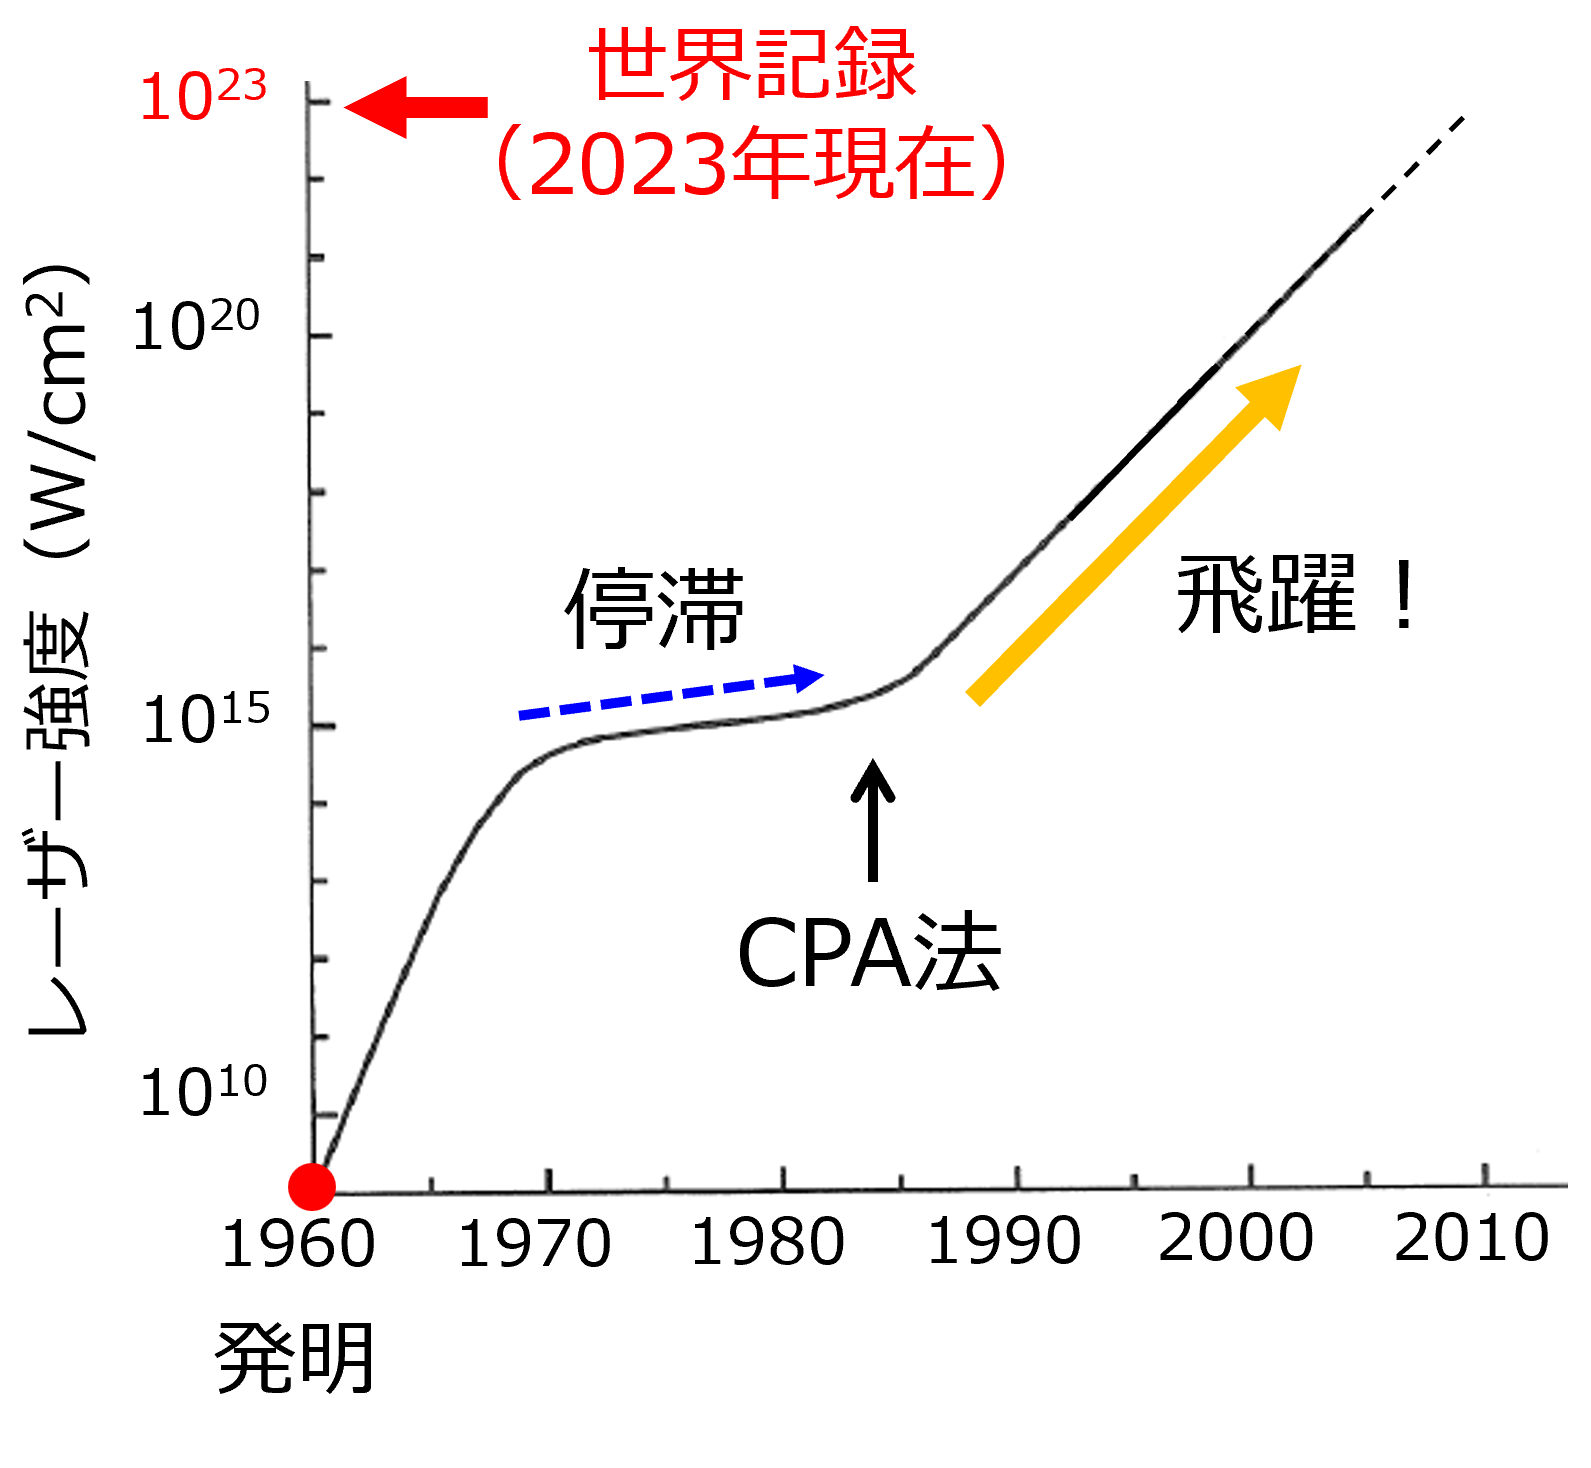
\includegraphics[scale=1]{./image/1-laser.png}
    \label{fig:1}
    \caption{高強度レーザー技術の発展。横軸は西暦、
    縦軸左は達成されたレーザーの最大集光強度(単位:W/cm$^2$)を示している。
    1985年のチャープパルス増幅法(Chirped Pulse Amplification,CPA法)の開発により、
    レーザー強度は飛躍的に増大している。
    縦軸右はレーザーにより電子が加速された際に得られる電子エネルギー(単位:eV(電子ボルト))を
    表しており、集光強度が10$^{18}$ W/cm$^{2}$で電子は相対論領域(速さ$v$~$c$、$c$:光速)となる。}
  \end{center}
\end{figure}


最近では、量子科学技術研究開発機構・関西光科学研究所のJ-KAREN-Pレーザー
\cite{t19,t20}などが
レーザーの最大集光強度$10^{21-22}\ \mathrm{W/cm^{2}}$領域の
フェムト秒極短パルス高強度レーザーを実現している。
このような高出力レーザーを物質に照射することで、物質はレーザーのパルス時間スケール(フェムト秒オーダ)で瞬時に電離してプラズマ化するとともに、
発生した多数の電子がレーザー光の光圧によりレーザー伝播方向に光速に近い速度にまで加速される。このような電子の相対論領域での運動により、
プラズマ中にはメガアンペア(MA)に達する大電流が駆動され、中性子パルサーに匹敵する数10キロテスラ(kT)の磁場が生成するとともに、
イオンと電子との電荷分離に起因して数10TV/mに達する電場が形成される。
この電場はイオンを数10 MeV/u(核子当たり)にまで加速させる。
すなわち、圧力が太陽の中心部の圧力(2000億気圧)の1/10に迫る、100億気圧オーダの高エネルギー密度プラズマが実験室レベルで生成可能である。


\begin{table}[H]
  \caption{レーザーの一覧}
  \centering
  \scalebox{0.85}{
    \begin{tabular}{lccccc} \hline \hline
      \multicolumn{5}{c}{レーザーの一覧} \\ \hline
      レーザー & 集光強度 & パルス幅 & 最大エネルギー & 波長 & 出力 \\ \hline 
      激光 XII(日) & $\sim 1\times 10^{19}\ \mathrm{W/cm^{2}}$ 
      & 0.1 $\sim$ 0.4 ns & 250 $\sim$ 1000 J & 527 or 1053 nm & 1 PW \\
      NIF(米) & $\sim 1\times 10^{16}\ \mathrm{W/cm^{2}}$  & 20 ns & 1.8J & 1053 nm & 500 TW \\ \hline
      LFEX(日)  & $ \sim 1\times 10^{19}\ \mathrm{W/cm^{2}}$ 
      & $0.5 \sim 20$ ps 
      & 2.5 kJ & 1053 nm & 2 PW \\ 
      OMEGA EP(米) & $ \sim 6 \times 10^{19}\ \mathrm{W/cm^{2}}$ 
      & $0.7 \sim 100$ ps 
      & 0.5 $\sim$ 2.3 kJ & 1053 nm & 不明 \\ \hline
      J-KAREN(日) & $ \sim 1\times 10^{22}\ \mathrm{W/cm^{2}}$ & 40 fs 
      & 30 J & 810 nm & 1 PW \\ %\hline \hline
      ELI(羅) & $\sim 1\times 10^{23}\ \mathrm{W/cm^{2}}$  & $\sim 17$ fs
      & $\sim$ 34 J & 800 $\sim$ 1030 nm & $\sim$ PW \\ \hline \hline
  \end{tabular}
  }
\end{table}

\subsection{医療・産業・学術への応用}
\subsubsection{イオン加速}
集光強度が$10^{18} W/ \rm{cm}^2$を上回る高強度レーザーを、厚さが数10nmから数µmのプラスチックや金属等の固体薄膜や、大気圧~大気圧の数倍に達する高密度ガスに照射することで、これらはフェムト秒のオーダで電離してプラズマ化する。このとき、電子はレーザー電場により電場方向に振動しながら、ローレンツ力の磁場成分(v × B)を受けてレーザー伝播方向(前方)に運動する。一方で、イオンは質量が大きいためレーザー場による運動は無視でき、その場に留まる。これにより、前方に運動した電子と残されたイオンとの間にはTV/mに達する超強電場が生成する。この電場により、イオンは電子に追随する形で前方に加速される。これらの現象は、物質表面のレーザー光照射領域(直径数µm~数10µm程度のレーザー集光径の領域)で起こり、電場が存在する領域もµmオーダの非常に局所的であるがTV/mの電場でµmのスケールで加速されたイオンは、典型的には核子当たり数MeVのエネルギーを得ることになる。これは、既存の大型加速器でイオンを加速した場合と比較して $10^3-10^4$倍の加速効率に相当する。すなわち、高強度レーザーを用いることで、イオン加速器の小型化が期待できる。\cite{ft6} このようなイオン加速手法は、レーザー駆動型のイオン加速手法と呼ばれており、レーザー集光強度の増大とともにプラズマ中で生成する電場強度も大きくなり、近年達成されつつある集光強度$10^{21−22} W/\rm{cm}^2$の領域では、100 TV/m の超強電場の生成が理論的に予測されており、これにより 100 MeV/u のイオン生成も視野に入っている。\cite{100Mev1, 100Mev2, 100Mev3}

\begin{figure}[H]
  \begin{center}
    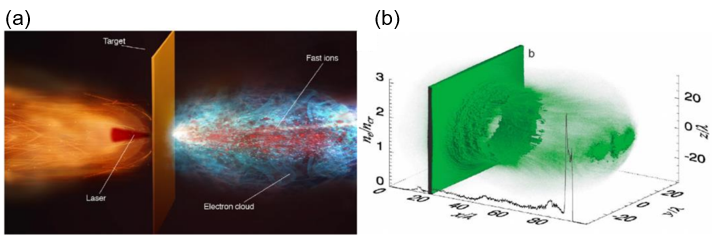
\includegraphics[scale=0.6]{./image/1-2-1.png}
    \label{fig:1-2-1}
    \caption{(a)はTNSA(TargetNormal Sheath Acceleration)機構を利用した、薄膜固体ターゲットにレーザーを照射した際に薄膜から高速イオンと電子雲が放出される図\cite{ion_Acceleration}。(b)はRPA(Radiation Pressure Acceleration,輻射圧加速)を利用したイオンの空間密度分布を示す\cite{ion_Acceleration_b}。}
  \end{center}
\end{figure}

したがって、この手法により、医療応用可能とされている 200MeV/u を上回るエネルギーまで短距離で加速できれば、これまで少数の大型施設でしか提供でき6なかった粒子線癌治療などの高度医療に新たな展開をもたらすことができるため、TNSA(TargetNormal Sheath Acceleration)\cite{10, 11, 12, 13, 14, 15}、 RPA(Radiation Pressure Acceleration,輻射圧加速)\cite{16, 17, 18}、CSA(Collisionless Shock Acceleration)といった代表的な加速機構\cite{19, 20, 21, 22, 23, 24, 25, 26} を中心に、世界的に研究が進められている。しかしながら、TNSAでは最大100MeVの加速実績はあるものの高品質には至らず、CSAではエネルギー幅が5%程度と高品質であるもののエネルギーは最大40MeV程度に留まっている。また、輻射圧加速(Radiation Pressure Acceleration, RPA)は現在達成できないレーザー強度領域である$(10^{23-24} W/\rm{cm}^2)$。



\subsubsection{レーザー核融合}
レーザーのパルス長がナノ秒領域となると、レーザーの集光強度領域は$(10^{15-16} W/\rm{cm}^2)$と
なる。このような高出力レーザーを燃料に照射することで、レーザー照射を受けた燃料の外
側は高温となり数千万気圧もの圧力が発生するため、球状の燃料はその中心に向かって圧
縮される(爆縮)。磁気閉じ込め方式の核融合では低密度のプラズマを長時間(1 秒以上)保
持することを目指すのに対し、レーザー核融合はプラズマがそれ自体の慣性でその場所に
留まっている間に核融合反応を起こしてエネルギーを取り出すことを目指している。レー
ザー核融合発電では、爆縮し、核融合反応が起こった燃料ペレットからは投入されたレーザ
ーエネルギーのQ倍のエネルギーが放出される。Q=1は投入したレーザーエネルギーと
発生した核融合エネルギーが均衡する点に相当するのでブレークイーブンと呼ばれる。これを達成するために様々な実験が世界で行われている\cite{NIF}。
2022年12月にNIF(ローレンスリバモア国立研究所)で、約2メガジュールのエネルギーを投入し、系約3.15メガジュールのエネルギーを発生させ、史上初のQ=1.5 を達成した。その後2023年に約2メガジュールの照射によって、これまでで最高となる3.88メガジュールのエネルギーを発生させることに成功し、続いて同年10月にも2回の実験で純増を達成した。

\begin{figure}[H]
  \begin{center}
    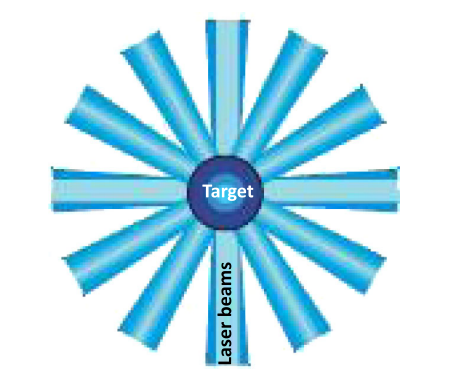
\includegraphics[scale=0.4]{./image/1-2-2.png}
    \label{fig:1-2-2}
    \caption{球状のシェルを対称的に複数のレーザー照射するICFの概略図\cite{NIF}}
  \end{center}
\end{figure}

\subsubsection{実験室宇宙物理}
高速プラズマ流による強磁場の生成、およびそれによる(電磁的)無衝突衝撃波は、宇宙において
普遍的にみられる現象である。ここで、対向する高速プラズマ流がぶつかることで生じるワイベル
不安定性(Weibel instability)が、衝突面近傍で強い磁場を生成し、この磁場により上述の無衝突
衝撃波が形成されると考えられている。一方で、高強度レーザーを物質に照射することで生成する
宇宙レベルの極限プラズマを実験室で再現する試み(実験室宇宙物理)において、ワイベル不安定
性の証拠となる「強磁場」の観測は困難な課題となっている。C. M. Huntington らは、プロトン・
ラジオグラフィー法を用いて、レーザー生成対向高速プラズマ流により、ワイベル不安定性に由来
する強磁場が生成した証拠を観測することに成功している。\cite{28}




高強度レーザーを照射する物質としては、これまで主に固体薄膜・高圧ガス等が用いられており、
これらにレーザーを照射することで、物質との境界層に高エネルギー密度プラズマを生成することが可能である。
一方で、このようにして生成されたプラズマは、$\tau_0 \sim L/C_s$
(\textit{L}:プラズマのサイズ、$C_s$:音速)で飛散してしまうため、応用研究の対象が
この時間スケールに収まる現象に限定される。

\subsection{構造性媒質と高強度レーザーの相互作用}
集光強度が$10^{19−21} W/ \rm{cm}^2$領域の高強度レーザーを様々な物質に照射することで
生成する数億気圧(Gbar)に達する高エネルギー密度プラズマは、同時にプラズマ中に駆動され
る超強電磁場や大電流とともに、これを利用した高エネルギー粒子加速やレーザー核融合、宇宙レ
ベルの現象など、様々な応用研究が期待される。一方、このような過程は、圧力の不均衡に起因し
た非定常性の強い過渡現象であり、それらはレーザーのパルス幅(~慣性時間)程度で散逸するこ
とから、応用研究もその時間内に成立するものに限られる。図\ref{fig:1-3-1}参照

\begin{figure}[H]
  \begin{center}
    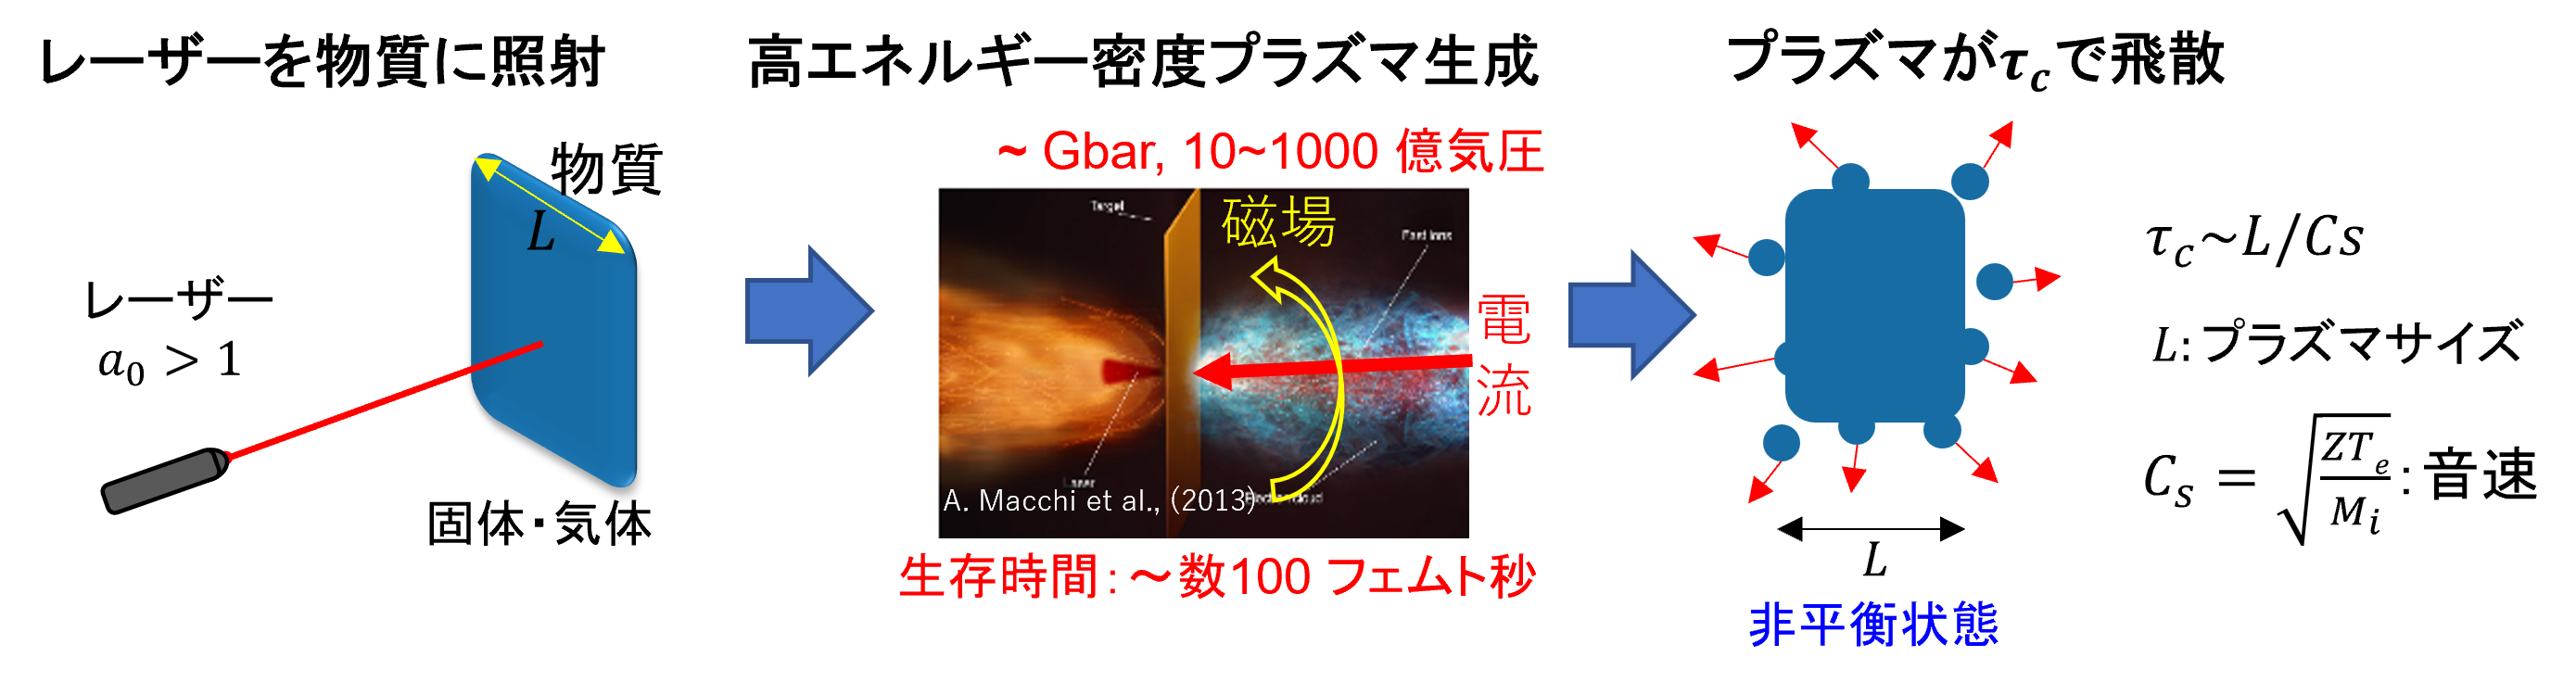
\includegraphics[scale=0.6]{./image/1-3-1.png}
    \label{fig:1-3-1}
    \caption{高強度レーザーを照射されたターゲット。通常、このような過程で高エネルギー密度プラズマが生成され\cite{ion_Acceleration}、$\tau c$程度の時間スケールで飛散し、応用研究の対象はその範囲内で起こりうる現象に限られる。}
  \end{center}
\end{figure}

これは、逆に、これまで慣性時間程度で飛散していた高エネルギー密度プラズマをこれを超えて
長時間“閉じ込める”ことができれば、上述の課題を克服して学術・応用研究の枠組みを広げるこ
とができる。この着想のもと、当研究室では、高強度レーザーを照射する物質として、一般に広く
用いられている固体薄膜 (厚さ数 10~ 数 100 nm に加工されたプラスチックや金属平板) に対し
て、物質の形状を球や円柱とすることで、比表面積 (質量に対する表面積の割合) が増大し、物質
表面とレーザーとの相互作用過程を通じて多彩な非線形現象を創出し得ると着想し、直径数 100
nm~µm の粒状固体物質 (クラスター) や、直径がサブ µm で高さが数 10µm オーダの円柱状ケイ
素(ロッド)が µm 間隔で複数配列した媒質(ロッド集合体)をターゲットとして選択し、これら
に集光強度領域が $10^{19−22} W/ \rm{cm}^2$ の高強度レーザーを照射する粒子シミュレーションと実験を実
施してきた。その結果、クラスターを用いたシミュレーションでは、高強度レーザー照射された水
素クラスター内外で起きる多段階素過程(衝撃波加速、相対論効果による陽子線の圧縮、および、
シース電場による陽子線の追加速)を同期させることで、光速の 65%に相当する 0.3 GeV のエ
ネルギーをもった高指向性の陽子線が生成することが明らかにされている(クラスター内衝撃波
駆動サブ GeV 級準単色陽子線生成)。\cite{29}本加速機構は CSBA 加速(Conversing Shock-induced
Blow-off Acceleration)として参照され、量子科学技術研究開発機構・関西光科学研究所で実施さ
れた検証実験において、CSBA 加速を指示する結果を得ている。\cite{30}また、臨界密度領域の高圧
の背景ガス(プラズマ)存在下において、直径がサブ µm オーダの円柱状物質(ロッド)に高強度
レーザーを照射すると、ロッドと背景ガスとの接触面近傍 (無衝突プラズマ境界層) において、無
衝突衝撃波により背景ガスイオンが加速される点や、電子の運動論的平衡による準安定静電孤立波
(BGK 波) が生成されるなど、ターゲット中に境界層を導入することで多彩な新機能が創出される
ことが明らかにされている。さらに、ロッド集合体の背景に臨界密度領域(大気圧の 10~100 倍程
度)の高圧ガスを導入したターゲットを用いることで、レーザー照射されたロッド集合体がクーロ
ン爆発を起こして膨張するとともに、それにより背景ガスが圧縮される。このとき、個々のロッド
周囲の2次元的衝撃波が、ホイヘンス・フレネルの原理と同様の原理で重ね合わされる結果、背景
ガス中(ロッド集合体外部)に準1次元的衝撃波が形成される。この衝撃波が形成する静電ポテン
シャルは、減衰することなく長時間にわたり衝撃波上流の背景ガスイオンを反射・加速する。\cite{uehara}
これにより、準単色高エネルギー背景ガスイオンが高フラックスで得られることが見いだされて
いる。また、ロッド集合体が存在する領域(ロッド領域)の外周に生じる電流ループにより、ロッ
ド領域内に数 kT に達する強磁場が生成することを見いだした。この磁場構造は、θ ピンチにより
ロッド領域内のプラズマを閉じ込める機能を有し、ピコ秒の時間スケールで準安定に存在すること
を明らかにした。\cite{IFSA}

\paragraph*{ロッド集合体}
当研究室では、上記のシミュレーションで見いだしたパラメータ領域をもとに、ナノ工学の専門家(謝辞:京都大学エネルギー理工学研究所・坂口浩司教授、京都大学工学研究科・深見一弘准教授)の協力のもと、最新の半導体製造技術を用いてシリコンロッド集合体を開発してきた。ロッド集合体は、直径サブ$\mu$mオーダで高さが数10$\mu$mの円柱状ケイ素が多数配列した構造を持つ(図\ref*{fig:1-3-2}参照)。具体的には、ネガ型もしくはポジ型レジスト液を塗布したシリコン基板上に、あらかじめ設計したデザインにしたがって電子線リソグラフィー技術により電子線で数nmのオーダで精緻に描画した後、現像を経てプラズマエッチングにより深堀りを行うことで作製する。プラズマエッチングでは、ボッシュプロセスと呼ばれる工程で高アスペクト比(高さ/直径:50-100)のロッド集合体の作製に成功している。図\ref*{fig:1-3-2}は、作製したロッド集合体の電子顕微鏡写真(SEM画像)である。高強度レーザーとの相互作用による相対論プラズマの生成と利用に関する研究分野では、レーザーのエネルギー吸収率を増大させる観点から、ターゲット表面にサブ$\mu$
mの構造を付与した物質の作製とそれを用いた実験研究が盛んに行われているが、高さが10 $\mu$mを上回るような高アスペクト比の構造物の作製は、リソグラフィーやプラズマエッチングの条件出しが非常に厳しいことから容易ではない。そのため、レーザーとの精緻な相互作用を目的としたロッド集合体の作製手法は当研究室が世界に先駆けて確立したものであり、レーザー照射用のターゲットとして世界中で注目を集めている。

\begin{figure}[H]
  \begin{center}
    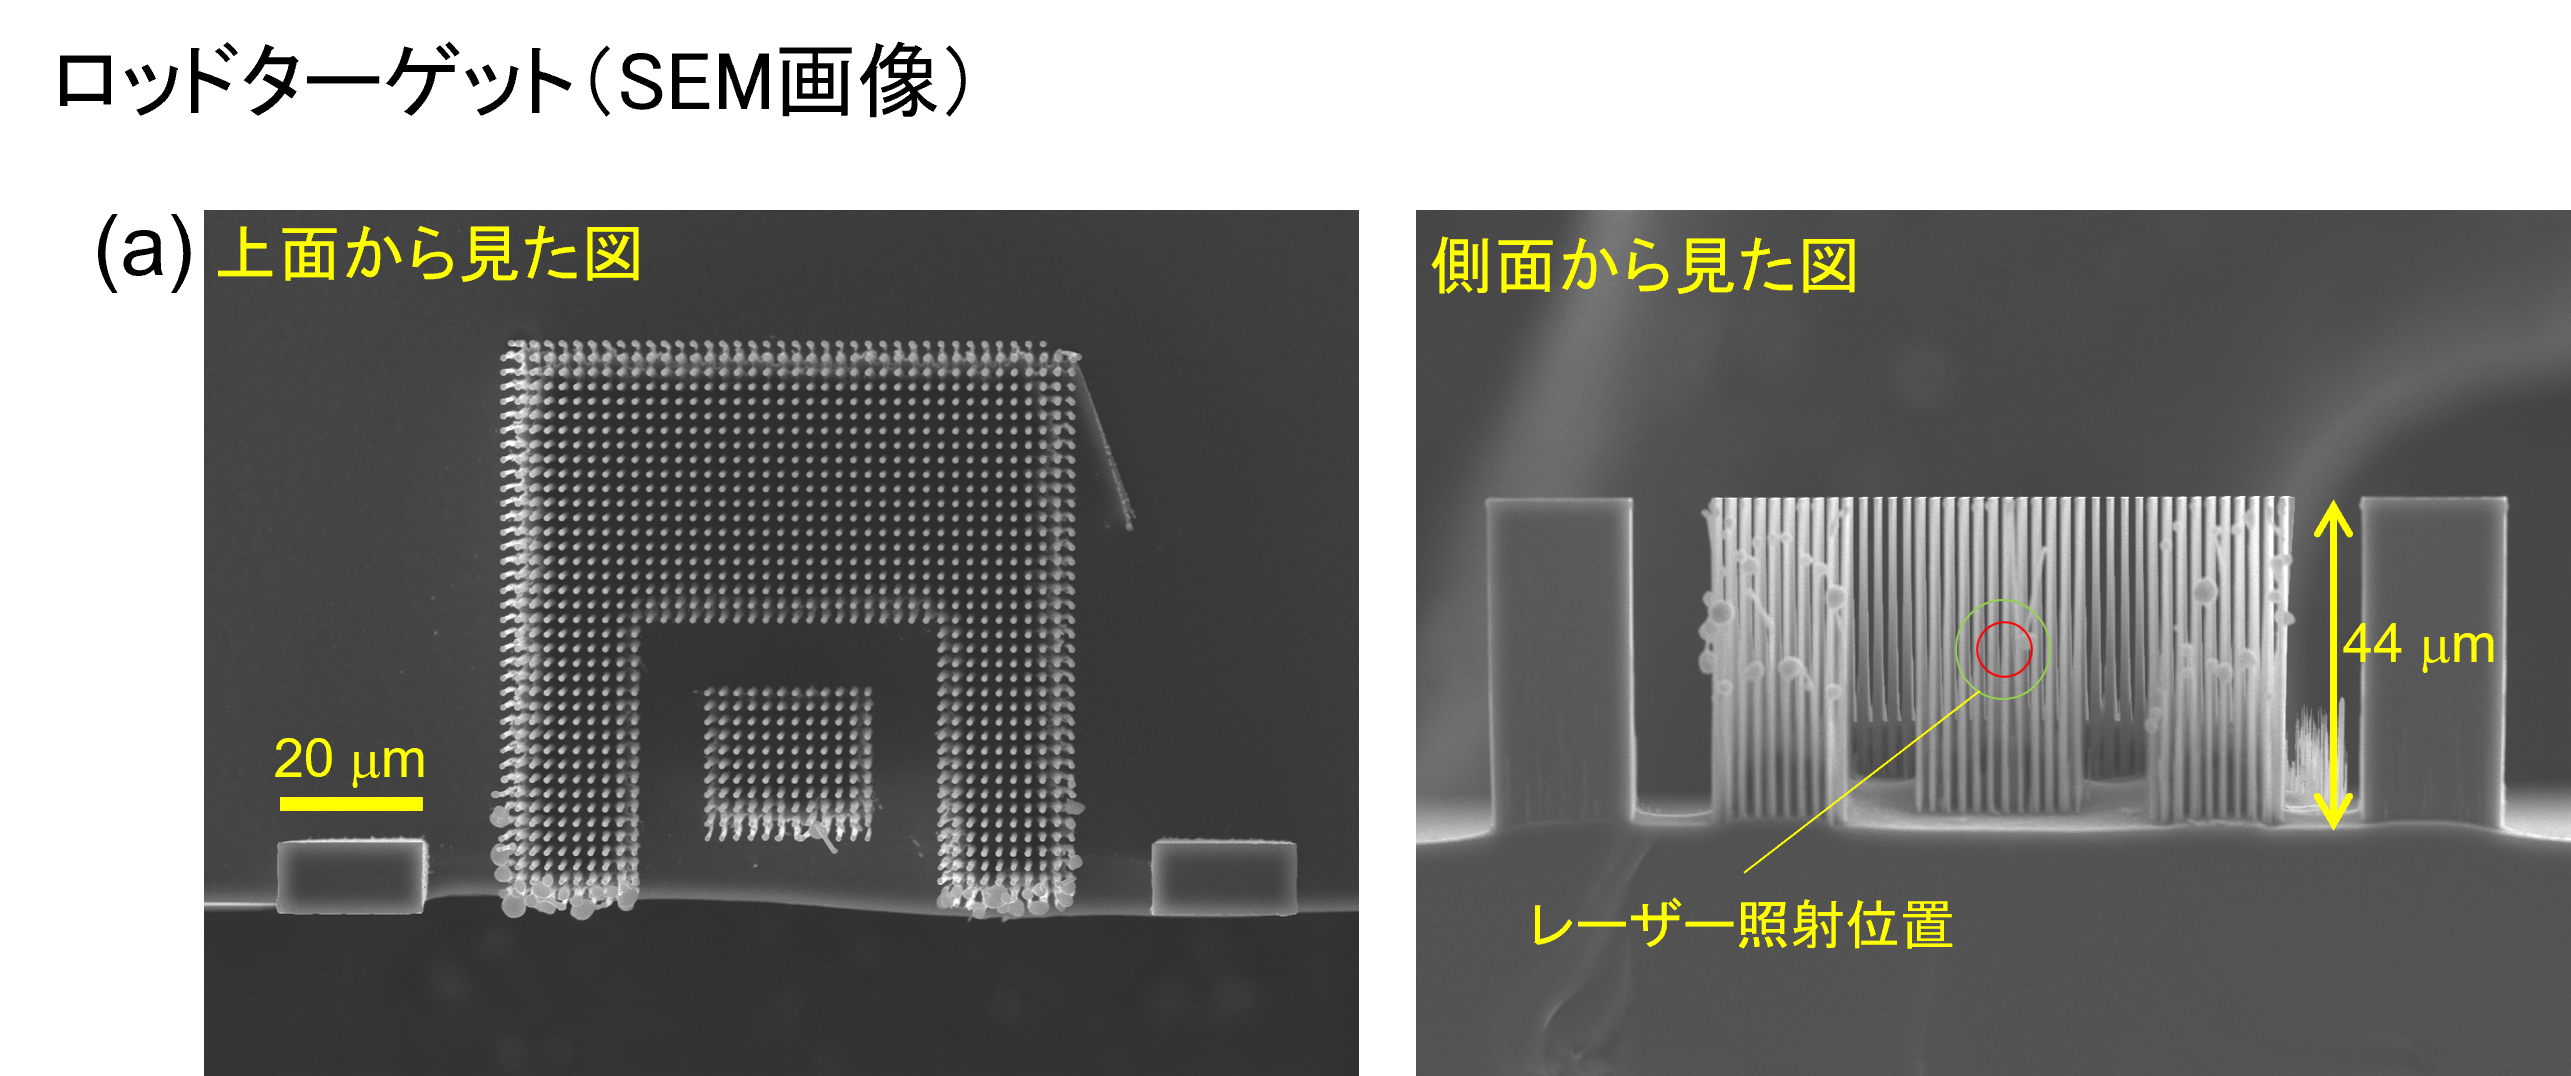
\includegraphics[scale=0.6]{./image/1-3/1-3_rod.png}
    \label{fig:1-3-2}
    \caption{ rod 集合体の電子顕微鏡写真。}
  \end{center}
\end{figure}

我々はこれまでに、ロッド集合体を用いて、京都大学化学研究所の T6 レーザーを用いたレーザー照射実験を複数回実施しており、生成する相対論プラズマの特性に関するデータベースを蓄積している。また、国際共同研究として、量子科学技術研究開発機構・関西光科学研究所の J-KAREN-P レーザー、理化学研究所の X 線自由電子レーザー SACLA のレーザーシステムを用いて、集光強度領
域が $10^{17−21} W/ \rm{cm}^2$ のフェムト秒極短パルス高強度レーザーを照射する実験を実施し、ロッド集
合体の電子のエネルギー分布特性や X 線小角散乱を用いたロッドの膨張速度の違い、生成する高
エネルギーイオンのエネルギー特性などを調べてきた。図 \ref*{fig:1-3-3}は、これまでに実施してきたレーザー照射実験の概要である。

\begin{figure}[H]
  \begin{center}
    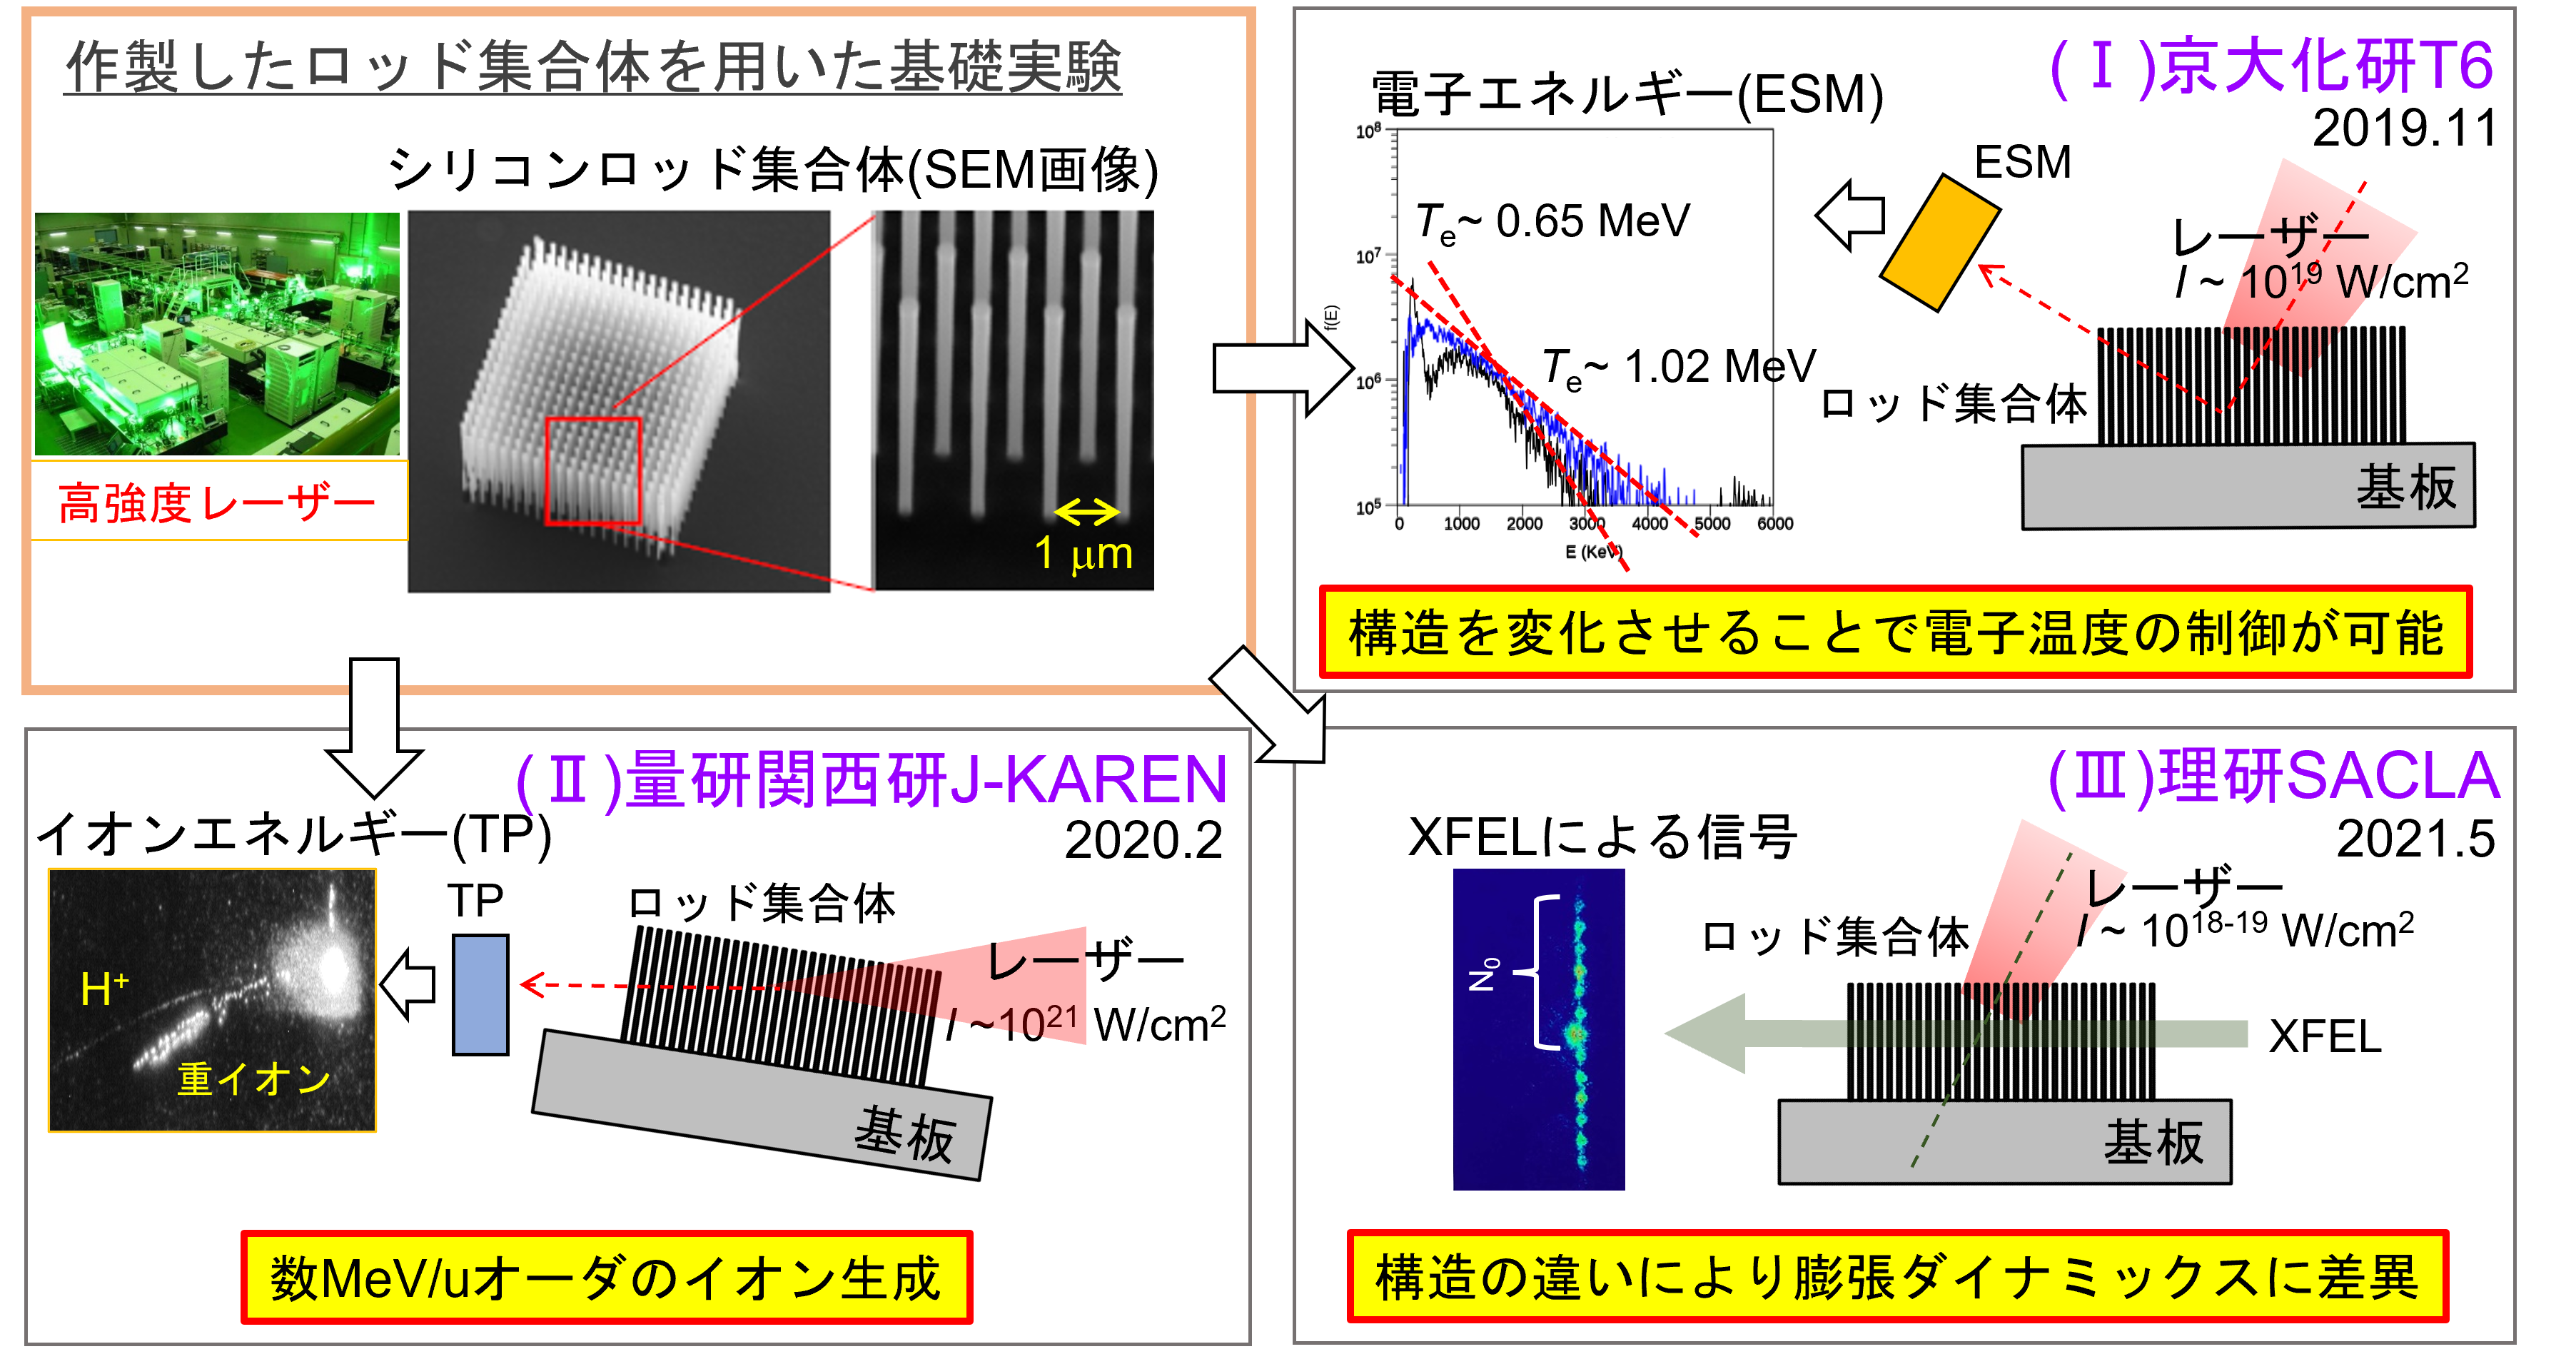
\includegraphics[scale=0.6]{./image/1-3/1-3_exp.png}
    \label{fig:1-3-3}
    \caption{ロッド集合体を用いた基礎実験。}
  \end{center}
\end{figure}

その結果、(i) スラブ状のシリコン基板のみの場合と、(ii) シリコンロッド集合体の場合で比較す
ると、高強度領域$(10^{19−21} W/ \rm{cm}^2)$において、ロッド集合体を用いた場合に高い電子温度が観測
され、ロッド集合体のレーザーエネルギー吸収率がスラブと比較して高くなることを示唆する実験
結果を得た。また、ロッド群の空間充填率を一定に保ってロッドの直径と間隔を変化させた場合、
ロッド径を小さくすることで高い電子温度が観測され、レーザーエネルギーの吸収率やロッドの膨
張速度に差異がみられることが確認できた。現在、本修士論文での主要な結論である、ロッド集合体とフェムト秒極短パルス高強度レーザーとの相互作用により実現する、レーザーのパルス時間を数桁上回るピコ秒スケールでの準定常強磁場(kT)生成の検証に向けた実験準備(京都大学化学研究所・大阪大学レーザー科学研究所との共同研究)が進められている。

\subsection{研究目的}

媒質に集光強度が $10^{20-21} W/ \rm{cm}^2$ を超えるレーザーを照射することで、媒質は即座に電離して相対論領域の電子と高エネルギーイオンからなる高エネルギー密度プラズマが生成し、電子の相対論領域での運動により、プラズマ中にはメガアンペア(MA)に達する大電流が駆動され、キロテスラ(kT)の磁場が生成するとともに、イオンと電子との電荷分離に起因して数10TV/mに達する電場が形成される。これらを利用し、核融合や線がん治療装置、実験室宇宙物理などに応用が期待される。一方、このようなプラズマはレーザーのパルス時間程度の短い時間で飛散するため、応用はこの時間スケールに限定される。したがって、この時間スケールをピコ秒からナノ秒のスケールに延ばすことは、 これまで、実現が困難とされてきたP-B熱核融合反応への応用などの応用研究の幅を広げることにつながる。この考えに基づき、本研究室では電子線リソグラフィーとプラズマエッチングプロセスを含む半導体技術によって、構造性媒質として直径がサブ µm で高さに対してあスペクトル比が40程度の高アスペクト比の円柱状ケイ素(シリコンロッド)が µm 間隔で多数配列した物質(ロッド集合体)を独自開発している。これらのロッド集合体を用いて、京都大学化学研究所の T6 レーザー、関西光科学研究所の J-KAREN-P レーザー、理化学研究所の X 線自由電子レーザー SACLA のレーザーシステムを用いて、京都大学化学研究所の T6 レーザー、関西光科学研究所の J-KAREN-P レーザー、理化学研究所の X 線自由電子レーザー SACLA のレーザーシステムを用いて、集光強度領域が $10^{17−21} W/\rm{cm}^2 $のフェムト秒極短パルス高強度レーザーを照射する実験を実施し、ロッド集合体の電子のエネルギー分布特性や X 線小角散乱を用いたロッドの膨張速度の違い、生成する高エネルギーイオンのエネルギー特性などを調査してきた。の結果、ロッド径・空間充填率・集合体のサイズといったロッド集合体を特徴付ける各種パラメータを適切に選択することで、ロッドの膨張速度やエネルギー吸収特性、電子エネルギーなどを制御可能であることを明らかにしてきた。これらを踏まえて、本研究では上記実験等で測定することが困難な局所的な磁場,電場の測定や、実験だけでは考察することが困難な磁場生成電流路形成のメカニズムを明らかにすることで、中性子を出さない究極の核融合である、水素・ホウ素熱核融合反応の実現を目指した、レーザー生成相対論プラズマの長時間制御を目的とする。この目的のもと相対論的電磁粒子コード EPIC3D\cite{m4}を用いて、レーザーと構造性媒質の相互作用による磁場生成電流路形成のメカニズムの解明と、プラズマ制御に向けた、より良いレーザーと構造性媒質のパラメータ(直径・高さ・空間充填率)を調べた。

\subsection{本論文の構成}

2章では高強度レーザーと物質の相互作用を支配する物理現象について説明する。
はじめにレーザー強度とパラメータについて記述し、それを踏まえ相対論領域(高強度レーザー領域)での電子の特徴的な運動について記述する。次にプラズマ内部への電磁波伝搬、電流のについて記述する。また、今回ロッドの基本性質を明らかにするために用いたエネルギー保存則と、導体極板間での電磁波伝搬についても記述する。$\\$
3章ではシミュレーションで扱う粒子コードの概要と各パラメータの規格化などについて記述する。$\\$
4章では、今回行ったシミュレーション結果を記載し、その考察をする。$\\$

\newpage

%%%%%%%%%%%%%%%%%%%%%%%%%%%%%%%%%%%%%%%% 2章 プラズマ、レーザーの理論 %%%%%%%%%%%%%%%%%%%%%%%%%%%%%%%%%%%%%%%%%%%%%%%%%%%%%%%%%%%%%%%%%%%%%%%%%%%%%%%%%%%%%%%%%%%%%%%%%%%

\section{レーザーと物質との相互作用を支配する物理}
  
  % \subsection{レーザー強度}
  % レーザーの強度を示すパラメーターとして規格化強度と呼ばれるパラメータが存在し、
  % これは電子の最大揺動速度と光速の比として定義される。
  % \begin{equation}
  %   a_0 = \frac{v_{\rm max}}{c}
  % \end{equation}
  % ここで$v_{\rm max}$は電子の最大揺動速度、$c$は光速を表す。
  % レーザー電磁場が直線変更であるとして、レーザー電場の
  \subsection{相対論的な電子の運動}
  CGS単位系を用いて電子の相対論的な運動方程式を記述すると
  \begin{equation}
    \label{eq:1}
    \frac{d\textit{\textbf{p}}}{dt} = e(\textit{\textbf{E}} + \frac{1}{c} 
    \textit{\textbf{v}} \times \textit{\textbf{B}})
  \end{equation}
  と表される。ここで、$\textit{\textbf{p}} = \gamma_e m_e \textit{\textbf{v}}$
  は電子の運動量を表し、$\textit{\textbf{v}}$は電子の速度を表す。
  また、$\gamma_e = \{ 1-(\frac{v}{c})^2 \}^{-\frac{1}{2}}$はローレンツ因子である。
  \textit{\textbf{E}}、\textit{\textbf{B}}はレーザー電場及び、磁場を表している。
  +y方向へレーザーが伝播すると仮定し、ベクトルポテンシャルを
  $\textit{\textbf{A}} = (\delta a_0 \textrm{cos}\phi,
  0、(1-\delta^2)^{\frac{1}{2}}a_0 \textrm{sin}\phi)$
  で表す。(\ref{eq:1})より、$(p_x、p_y、p_z)$と$(x、y、z)$は以下のように表される。
  \begin{equation}
  \label{eq:2}
    \left\{
      \begin{array}{ll}
        p_x = \delta a_0 \textrm{cos}\phi & \\
        p_y = \frac{a_0^2}{4}[1 + (2\delta^2 - 1)\textrm{cos2}\phi ] & \\
        p_z = (1-\delta^2)^{\frac{1}{2}}
      \end{array}
    \right.
  \end{equation}

  \begin{equation}
    \label{eq:3}
      \left\{
        \begin{array}{ll}
          x = \delta a_0 \textrm{sin}\phi & \\
          y = \frac{a_0^2}{4}[\phi + (\delta^2 - \frac{1}{2})\textrm{sin2}\phi ] & \\
          z = -(1-\delta^2)^{\frac{1}{2}} a_0 \textrm{cos}\phi 
        \end{array}
      \right.
    \end{equation}
  \begin{figure}[H]
    \begin{center}
      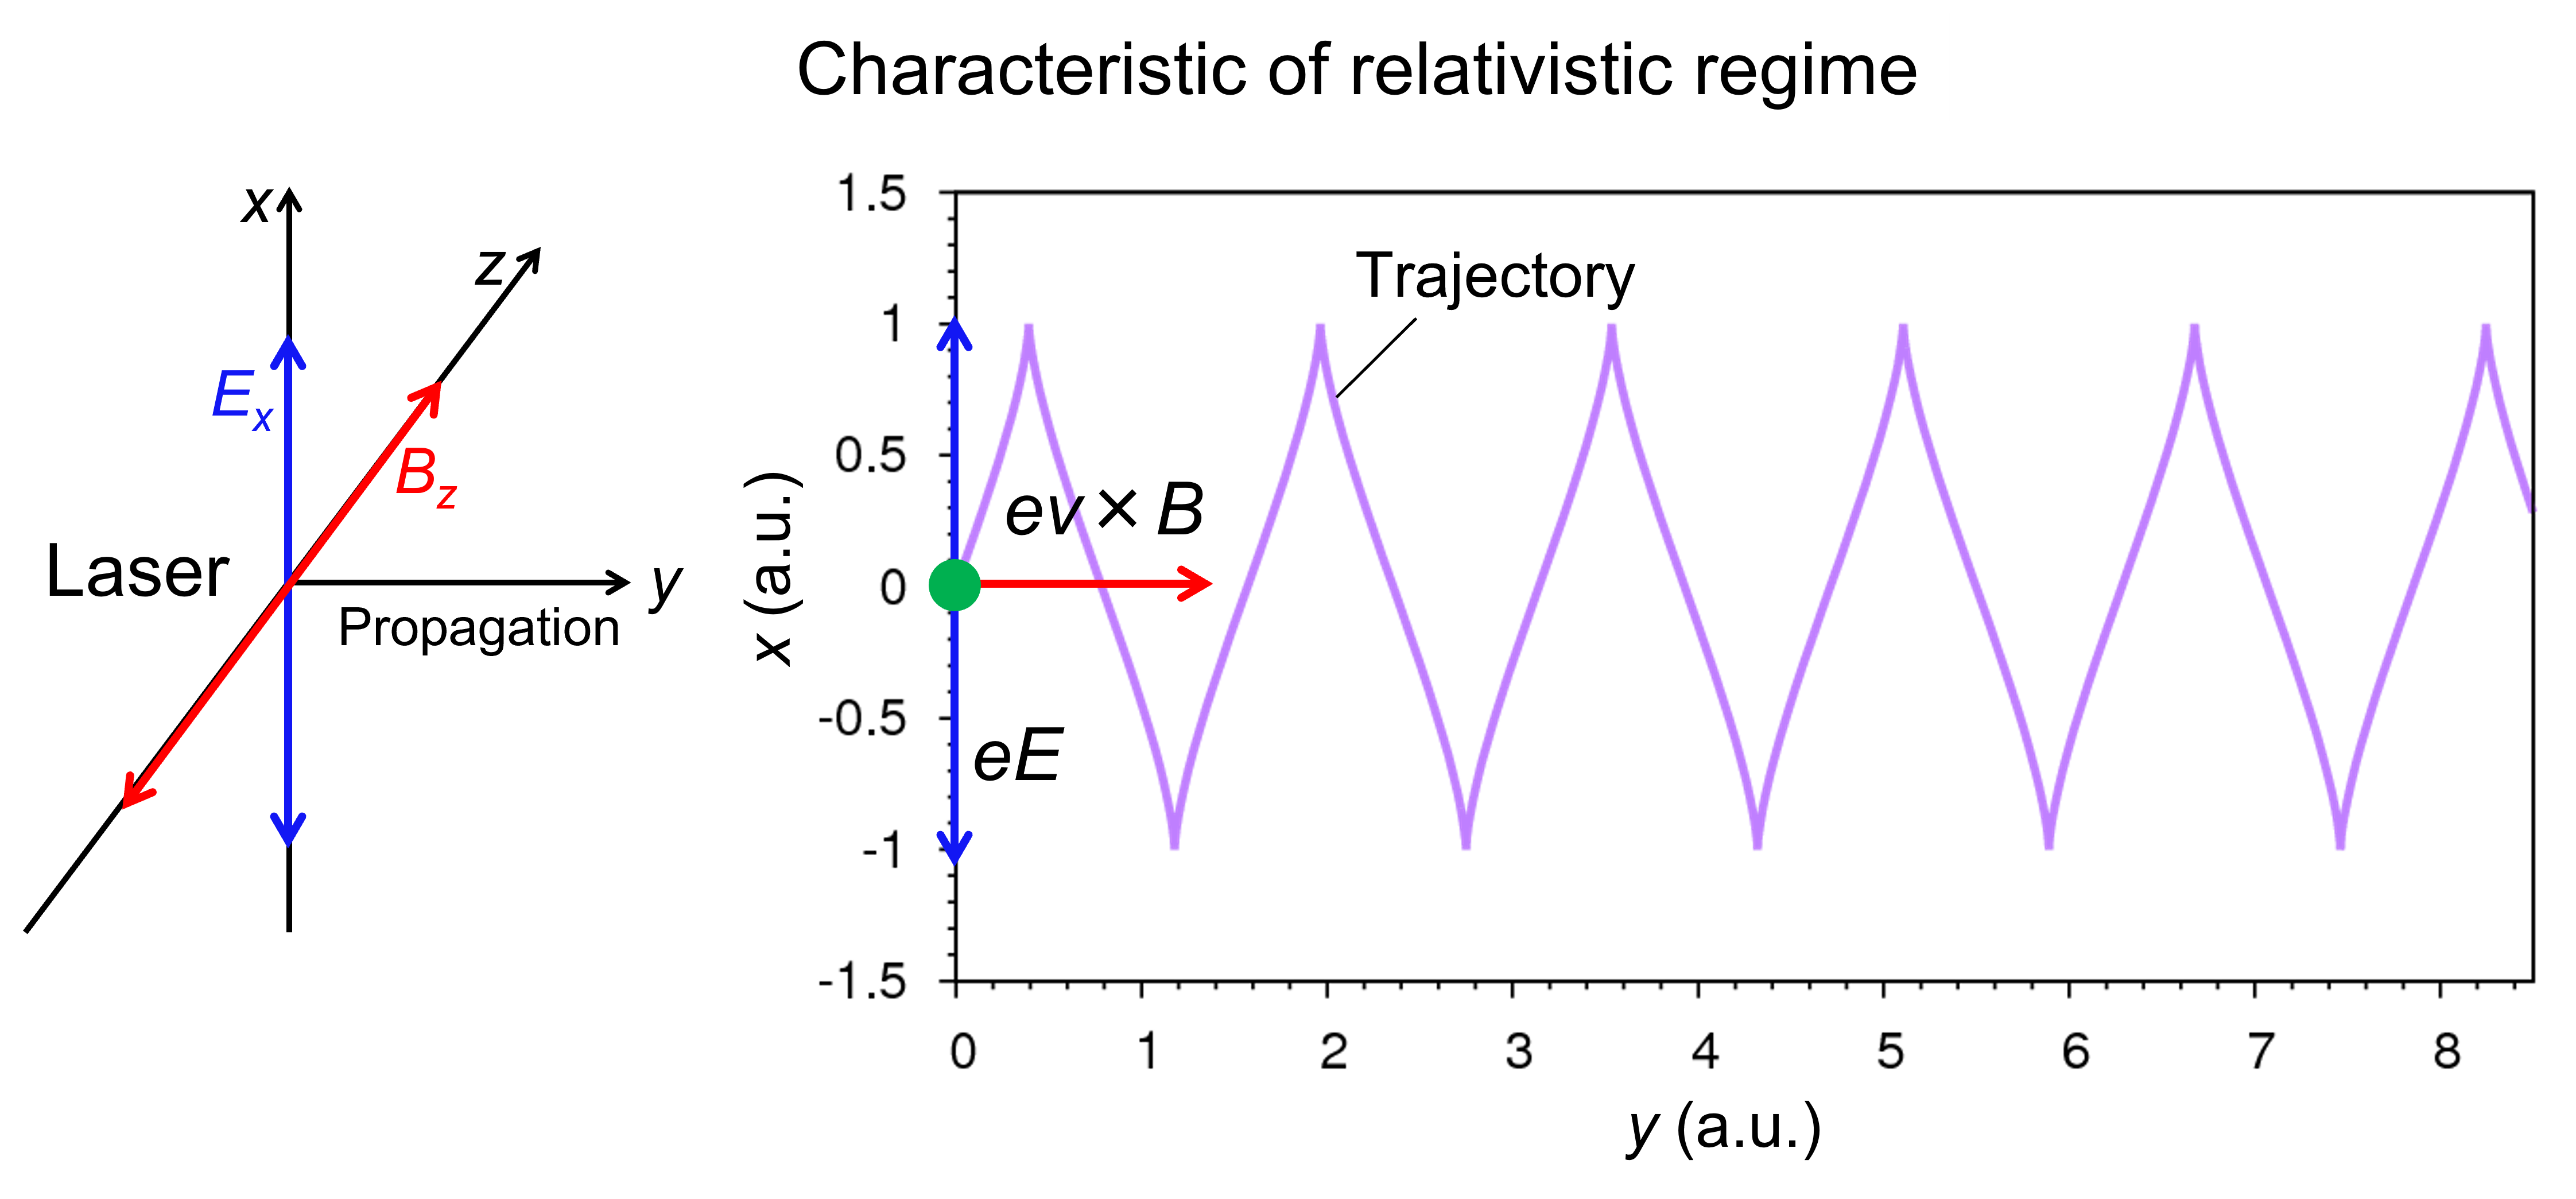
\includegraphics[keepaspectratio,width=\linewidth]{./image/2-1/2-1_propagation.png}
      \label{}
      \caption{
        直線偏光のレーザーが照射された場合の電子軌道を(x、y)平面に描かせた図。レーザーは+y方向に伝播する。
        電子は+y方向にローレンツ力の磁場成分を受けて動く。また、レーザー電場によってx方向に振動を行う。
        (Study of nonlinear structures and dynamics in collisionless plasmas created by the 
        interaction between high power laser and cluster medium より引用)
      }
    \end{center}
  \end{figure}   
  (\ref{eq:3})から分かる通り、規格化強度$a_0$が1より大きい相対論領域において、電子の運動はy方向が支配的となる。
  \subsection{分散関係及びカットオフ密度}
  \rm Maxwell方程式は電場を$\bm{E}$、磁場を$\bm{B}$、電流密度を$\bm{j}$として
  \begin{eqnarray}
    \label{eq:4}
    \nabla \times \textit{\textbf{E}} &=& 
    -\frac{1}{c}\frac{\partial \textbf{\textit{\textbf{B}}}}{\partial t}\\
    \label{eq:5}
    \nabla \times \textit{\textbf{B}} &=& \frac{4\pi}{c} 
    \textbf{\textit{j}} +\frac{1}{c}\frac{\partial \textit{\textbf{B}} }{\partial t}
  \end{eqnarray}
  で与えられる。ここでcは光速を表し、y方向に伝播する電磁波を考えると
  \begin{eqnarray}
    \label{eq:6}
    \textit{\textbf{E}}&=&E_0 e^{i(ky-\omega_L t) \textit{\textbf{x}}}\\
    \label{eq:7}
    \textit{\textbf{B}}&=&B_0 e^{i(ky-\omega_L t) \textit{\textbf{z}}}
  \end{eqnarray}
  で与えられる。ここで$\omega_L$は電磁場(レーザー)の周波数、\textit{k}は波数である。
  これらを(\ref{eq:4})、(\ref{eq:5})のMaxwell方程式に代入すると
  \begin{eqnarray}
    \label{eq:8}
    ckE&=&\omega_L B\\
    \label{eq:9}
    ikB&=&\frac{4\pi}{c}j + \frac{i\omega_L}{c} \textit{E}
  \end{eqnarray}
  (\ref{eq:8})、(\ref{eq:9})より\textit{B}を消去すると以下の式
  \begin{equation}
    \label{eq:10}
    j=\frac{i(c^2 k^2 -\omega_L^2)}{4\pi \omega_L}E
  \end{equation}
  が得られる。ここで\textit{i}は虚数単位を表す。
  また、一方で電子の運動方程式については、(\ref{eq:1})より、電子の初速を0とすると
  \begin{equation}
    \label{eq:11}
    m_e \frac{\textit{dv}}{\textit{dt}}=-e\textit{E}
  \end{equation}
  となり、この式より
  \begin{equation}
    \label{eq:12}
    \textit{v}=-{\frac{e^2 n_e}{m_e} \frac{E}{i\omega_L}}
  \end{equation}
  となる。ここで電子密度を$n_e$とすると、電流密度$j$は$j=en_e v$で表され、
  (\ref{eq:12})より
  \begin{equation}
    \label{eq:13}
    j=-\frac{e^2 n_e}{m_e} \frac{E}{i\omega_L}
  \end{equation}
  となる。(\ref{eq:10})と(\ref{eq:13})を比較することで
  \begin{equation}
    \label{eq:14}
    \omega_L^2={\omega_p}^2+c^2 k^2
  \end{equation}
  が得られ、これがプラズマ中における電磁場の分散関係となる。ここで$\omega_p$は
  プラズマ周波数と呼ばれ、
  \begin{equation}
    \label{eq:15}
    \omega_p = \sqrt{\frac{4\pi n_e e^2}{m_e}}
  \end{equation}
  で表される。また、式(\ref{eq:14})を$k$について解くことで
  \begin{equation}
    \label{eq:16}
    k=\frac{1}{c} \sqrt{\omega_L^2 - {\omega_p}^2}
  \end{equation}
  これより、$\omega_p > \omega_L$の場合、プラズマ内部での電磁波の波数$k$が虚数となり、電磁波が指数関数的に減衰することが分かる。
  この臨界密度のことを特にカットオフ密度と呼び、一般に$n_c$で表記する。
  \begin{equation}
    \label{eq:17}
    n_c=\frac{m_e \omega_L^2}{4\pi e^2}
  \end{equation}
  またこの時の電場\textit{E}は
  \begin{equation}
    \label{eq:18}
    E\propto \rm{exp}(\frac{i}{c} \sqrt{\omega_L^2 - {\omega_p}^2})z
  \end{equation}
  で表されるため、レーザー電場の大きさが1/\textit{e}になる長さ$\delta$は
  \begin{equation}
    \label{eq:19}
    \delta = \frac{c}{\sqrt{{\omega_p}^2-{\omega_L}^2}}
  \end{equation}  
  となる。特に${\omega_p}^2>>{\omega_L}^2$のような高密度プラズマでは
  \begin{equation}
    \label{eq:20}
    \delta = \frac{c}{\omega_p}
  \end{equation}
  となる。この$\delta$をスキン長(表皮距離)と呼ぶ。
  また、相対論領域の高密度プラズマを扱う場合、ローレンツ因子がかかる。
  \begin{equation}
    \label{eq:21}
    \omega_p=\sqrt{\frac{4\pi ne^2}{m\gamma}}
  \end{equation} 

  \subsection{レーザー強度}
  真空中の電場と磁場の 波動方程式は、
  
  \begin{eqnarray}
    \label{eq:2-3-1}
    \nabla \cdot \textit{\textbf{E}} &=& 4\pi r\\
    \label{eq:2-3-2}
    \nabla \cdot \textit{\textbf{B}} &=& 0
  \end{eqnarray}
  
  であり、(\ref{eq:4}),(\ref{eq:5})とMaxwell方程式を用いると
  
  \begin{eqnarray}
    \label{eq:2-3-3}
    % 1=1
    \nabla ^{2} \textit{\textbf{E}} - \frac{1}{c^2} \frac{\partial ^{2} \textit{\textbf{E}}}{\partial t^2} = 0\\
    \label{eq:2-3-4}
    \nabla ^2 \textit{\textbf{B}} - \frac{1}{c^2} \frac{\partial ^2 \textit{\textbf{B}}}{\partial t^2}=0  
  \end{eqnarray}
  
  とすることができる。本研究では、レーザー電場をx方向、磁場をz方向、進行方向をy方向に設定するため、ここでもそれに基づき計算を行う。アンテナをy=0の位置に置き、レーザーを照射した場合を考えると、レーザーによって生じる電場と磁場はそれぞれ、
  
  \begin{eqnarray}
    \label{eq:2-3-5}
    \textit{\textbf{E}}=E_0 \rm{sin} \lparen \omega t -\frac{2\pi}{\lambda} y \rparen \hat{\textit{\textbf{x}}}\\
    \label{eq:2-3-6}
    \textit{\textbf{B}}=B_0 \rm{sin} \lparen \omega t -\frac{2\pi}{\lambda} y \rparen \hat{\textit{\textbf{z}}}
  \end{eqnarray}
  
  と合わせることができる。これらは式(\ref{eq:2-3-3})(\ref{eq:2-3-4})を満たす解となる。
  また、電磁場の平均エネルギーは密度uは、
  \begin{eqnarray}
    \label{eq:2-3-7}
    u = \frac{1}{8 \pi} \lparen <E_x^2>  + <B_z^2> \rparen
  \end{eqnarray}
  
  となる。$<E_x^2>$,$<B_z^2>$はぞれぞれ、レーザー周期にわたり時間平均を行った値である。また式(\ref{eq:2-3-5}),(\ref*{eq:2-3-6})から
  
  \begin{eqnarray}
    <E_x^2>= \frac{E_0^2}{2}\\
    <B_z^2>=<E_x^2>
  \end{eqnarray}
  
  となるので、これらを式(\ref*{eq:2-3-7})に代入すると、
  \begin{eqnarray}
    u= \frac{E_0^2}{8 \pi}
  \end{eqnarray}
  
  と書食ことができる。レーザー強度$I$はエネルギー密度の流速であることからレーザー強度は$c$を光速とすると、
  
  \begin{eqnarray}
    I=uc= \frac{E_0^2 c}{8 \pi}
  \end{eqnarray}
  
  となる。この表式では$I$の単位は$[erg/cm^2\cdot s]$である。CGS-Gauss系を用いるときは$erg$を$J$に直せばいいので、その場合の単位は$[erg/cm^2]$となり、
  
  \begin{eqnarray}
    I= \frac{E_0^2 c}{8 \pi} \times 10^{-7}
  \end{eqnarray}
  である。



  \subsection{ポンデロモーティブ力}

  \paragraph*{直線偏光の場合}
  
  \begin{eqnarray}
    \label{eq:2-4-1}
    \textit{\textbf{E}} =E(x,y) \rm{sin} \omega _0 \textit{t} \hat{\textit{\textbf{x}}}
  \end{eqnarray}
  
  この式の$E(x,y)$はx,y方向空間依存性を含む。ここで、運動方程式は書く。
  
  \begin{eqnarray}
    \label{eq:2-4-2}
    m \frac{d \textit{\textbf{v}}}{dt} =-e \lparen \textit{\textbf{E}} + \frac{1}{c}\textit{\textbf{v}} \times \textit{\textbf{B}} \rparen
  \end{eqnarray}
  
  一次のオーダーでx方向に運動する電子を考える。
  これに式(\ref*{eq:2-4-1})を代入し$\textit{\textbf{v}} \times \textit{\textbf{B}}$を無視すると
  
  \begin{eqnarray}
    m \frac{d \textit{\textbf{v}}_1}{dt} &=& -e E(x,y) \rm{sin} \omega _0 \textit{t} \hat{\textit{\textbf{x}}}\\
    \textit{\textbf{v}}_1 &=& \frac{e E(x,y)}{m \omega _0} \rm{cos} \omega _0 \textit{t} \hat{\textit{\textbf{x}}}\\
    \delta \textit{\textbf{x}} &=& \frac{e E(x,y)}{m \omega _0^2} \rm{sin} \omega _0 \textit{t} \hat{\textit{\textbf{x}}}
  \end{eqnarray} 
  
  次にE(x,y)を二次のオーダーまで展開すると
  
  \begin{eqnarray}
    E(x,y) = E(x,y) + \delta x \frac{\partial E(x,y)}{\partial x}
  \end{eqnarray}
  
  また、Maxwell方程式より
  
  \begin{eqnarray}
    \nabla \times \textit{\textbf{E}} &=& - \frac{1}{c} \frac{d \textit{\textbf{B}}}{dt}\\
    \frac{d \textit{\textbf{B}}}{dt} &=& -c \nabla \times E(x,y) \rm{sin} \omega _0 \textit{t} \hat{\textit{\textbf{x}}}\\
    \textit{\textbf{B}} &=& \frac{c}{\omega _0} \rm{cos}\omega _0 \textit{t} \lparen \nabla \times E(x,y) \hat{\textit{\textbf{x}}} \rparen
  \end{eqnarray}
  
  これらを式(\ref{eq:2-4-2})に代入し、二次のオーダーでx方向に運動する電子を考える。
  
  \begin{eqnarray}
    && m \frac{d \textit{\textbf{v}}_2}{dt} = -e \lparen \delta x \frac{\partial E(x,y)}{\partial x} \rm{sin} \omega _0 \textit{t} \hat{\textit{\textbf{x}}} + \frac{1}{c} \textit{\textbf{v}}_1 \times \textit{\textbf{B}} \rparen\\
    &=& -e \lparen \frac{e \rm{sin^2} \omega _0 \textit{t}}{m \omega _0^2} E(x,y) \frac{\partial E(x,y)}{\partial x}  \hat{\textit{\textbf{x}}} + \frac{e \rm{cos^2} \omega _0 \textit{t}}{m \omega _0^2} E(x,y) \frac{\partial E(x,y)}{\partial y} \hat{\textit{\textbf{y}}}\rparen\\
    \label{eq:2-4-3}
    &=& - \frac{e^2 }{2 m \omega _0^2} \rm{sin^2} \omega _0 \textit{t} \frac{\partial }{\partial \textit{x}} \textit{E}(x,y)^2 \hat{\textit{\textbf{x}}} - \frac{e^2 }{2 \textit{m} \omega _0^2} \rm{cos^2} \omega _0 \textit{t} \frac{\partial }{\partial \textit{y}}\textit{E}(x,y)^2 \hat{\textit{\textbf{y}}}
  \end{eqnarray}
  
  となる。上式は
  \begin{eqnarray}
    \nabla \times E(x,y) \hat{\textit{\textbf{x}}} &=& -\frac{\partial E(x,y)}{\partial y}\hat{\textit{\textbf{z}}}\\
    \textit{\textbf{v}}_1 \times \textit{\textbf{B}} &=& \frac{ce \rm{cos^2} \omega _0 \textit{t}}{m \omega _0^2} E(x,y) \frac{\partial E(x,y)}{\partial y} \hat{\textit{\textbf{y}}}
  \end{eqnarray}
  の2式を用いた。式(\ref{eq:2-4-3})よりレーザー光(電磁場)の伝播方向であるy方向に働く力は
  
  \begin{eqnarray}
    f_{//}=- \frac{e^2 }{4 \textit{m} \omega _0^2}  (1 + \rm{cos} 2 \omega _0 \textit{t} )\frac{\partial }{\partial \textit{y}}\textit{E}(x,y)^2 \hat{\textit{\textbf{y}}}
  \end{eqnarray}
  
  であり、これを直線変更の場合のポンデロモーティブ力という。これは第一項の主成分と第二項の振動成分からなる。この力はイオンと電子の電荷に関係なく同じ方向に働くが、質量mの差によってイオンと比べ電子は強くこの力を受ける。
  
  \paragraph*{円偏光の場合}
  
  \begin{eqnarray}
    \label{eq:2-4-4}
    \textit{\textbf{E}} &=& \frac{1}{\sqrt[]{2}} E(x,y,z) \rm{sin} \omega _0 \textit{t} \hat{\textit{\textbf{x}}} + \frac{1}{\sqrt[]{2}} E(x,y,z) \rm{cos} \omega _0 \textit{t} \hat{\textit{\textbf{z}}}\\
    E_L &=& \frac{1}{\sqrt[]{2}} E(x,y,z) 
  \end{eqnarray}
  
  直線偏光の場合と同様に運動方程式から、一次のオーダーでxz平面上を運動する電子を考えと、
  
  \begin{eqnarray}
    \textit{\textbf{v}}_x &=& \frac{e E_L}{m \omega _0} \rm{cos} \omega _0 \textit{t} \hat{\textit{\textbf{x}}}\\
    \delta \textit{\textbf{x}} &=& \frac{e E_L}{m \omega _0^2} \rm{sin} \omega _0 \textit{t} \hat{\textit{\textbf{x}}}\\
    \textit{\textbf{v}}_z &=& - \frac{e E_L}{m \omega _0} \rm{sin} \omega _0 \textit{t} \hat{\textit{\textbf{z}}}\\
    \delta \textit{\textbf{z}} &=& \frac{e E_L}{m \omega _0^2} \rm{cos} \omega _0 \textit{t} \hat{\textit{\textbf{z}}}
  \end{eqnarray}
  
  となり、次にE(x,y,z)を二次のオーダーまで展開すると
  
  \begin{eqnarray}
    E(x,y,z) = E_L + \delta x \frac{\partial E_L}{\partial x} + \delta z \frac{\partial E_L}{\partial z}
  \end{eqnarray}
  
  また、Maxwell方程式より
  
  \begin{eqnarray}
    \nabla \times \textit{\textbf{E}} &=& - \frac{1}{c} \frac{d \textit{\textbf{B}}}{dt}\\
    \frac{d \textit{\textbf{B}}}{dt} &=& -c \nabla \times (\frac{1}{\sqrt[]{2}} E(x,y,z) \rm{sin} \omega _0 \textit{t} \hat{\textit{\textbf{x}}} + \frac{1}{\sqrt[]{2}} E(x,y,z) \rm{cos} \omega _0 \textit{t} \hat{\textit{\textbf{z}}})\\
    \textit{\textbf{B}} &=& \frac{c}{\sqrt[]{2} \omega _0} \rm{cos}\omega _0 \textit{t} \lparen \nabla \times E(x,y,z) \hat{\textit{\textbf{x}}} \rparen - \frac{c}{\sqrt[]{2} \omega _0}\rm{sin}\omega _0 \textit{t} \lparen \nabla \times E(x,y,z) \hat{\textit{\textbf{z}}} \rparen 
  \end{eqnarray}
  
  これらを式(\ref{eq:2-4-2})に代入し、二次のオーダーでx方向に運動する電子を考える。
  
  \begin{eqnarray}
    m \frac{d \textit{\textbf{v}}_2}{dt} &=& -e  \Biggl(\delta x \frac{\partial \textit{E}_\textit{L}}{\partial x} ( \rm{sin} \omega _0 \textit{t} \hat{\textit{\textbf{x}}} + \rm{cos} \omega _0 \textit{t} \hat{\textit{\textbf{z}}}) + \delta z \frac{\partial \textit{E}_\textit{L}}{\partial z} ( \rm{sin} \omega _0 \textit{t} \hat{\textit{\textbf{x}}} + \rm{cos} \omega _0 \textit{t} \hat{\textit{\textbf{z}}}) + \frac{1}{c} \textit{\textbf{v}}_1 \times \textit{\textbf{B}}  \Biggr)\nonumber\\
    \label{eq:2-4-5}
    &=&- \frac{e^2 }{m \omega _0^2} \textit{E}_\textit{L}\frac{\partial \textit{E}_\textit{L}}{\partial \textit{y}}\hat{\textit{\textbf{y}}}
  \end{eqnarray}
  
  
  となる。上式は
  \begin{eqnarray}
    \nabla \times \textit{\textbf{E}} &=& \frac{\partial \textit{E}_L}{\partial y} \rm{cos} \omega _0 \textit{t} \hat{\textit{\textbf{x}}} + (\frac{\partial \textit{E}_L}{\partial \textit{z}} \rm{sin} \omega _0 \textit{t} - \frac{\partial \textit{E}_L}{\partial \textit{x}} \rm{cos} \omega _0 \textit{t})\hat{\textit{\textbf{y}}} -\frac{\partial \textit{E}_L}{\partial \textit{y}} \rm{sin} \omega _0 \textit{t} \hat{\textit{\textbf{z}}}\\
    \textit{\textbf{v}}_1 \times \textit{\textbf{B}} &=& \frac{c e \textit{E}_\textit{L}}{m \omega _0^2} (\frac{\partial \textit{E}_\textit{L}}{\partial \textit{z}} \rm{sin}\omega _0 \textit{t}\rm{cos}\omega _0 \textit{t} + \frac{\partial \textit{E}_\textit{L}}{\partial \textit{x}}\rm{sin^2}\omega _0 \textit{t})\hat{\textit{\textbf{x}}}    \nonumber\\
    &+& \frac{c e \textit{E}_\textit{L}}{m \omega _0^2} (\frac{\partial \textit{E}_\textit{L}}{\partial \textit{y}} \rm{sin^2}\omega _0 \textit{t} + \frac{\partial \textit{E}_\textit{L}}{\partial \textit{y}}\rm{cos^2}\omega _0 \textit{t})\hat{\textit{\textbf{y}}}   \nonumber \\
    &+& \frac{c e \textit{E}_\textit{L}}{m \omega _0^2} (\frac{\partial \textit{E}_\textit{L}}{\partial \textit{x}} \rm{sin}\omega _0 \textit{t}\rm{cos}\omega _0 \textit{t} + \frac{\partial \textit{E}_\textit{L}}{\partial \textit{z}}\rm{cos^2}\omega _0 \textit{t})\hat{\textit{\textbf{z}}}
  \end{eqnarray}
  の2式を用いた。式(\ref{eq:2-4-5})よりレーザー光(電磁場)の伝播方向であるy方向に働く力は
  
  \begin{eqnarray}
    f_{//}=- \frac{e^2 }{4 \textit{m} \omega _0^2}  \frac{\partial }{\partial \textit{y}}\textit{E}(x,y,z)^2 \hat{\textit{\textbf{y}}}
  \end{eqnarray}
  
  であり、これを円偏光の場合のポンデロモーティブ力という。直線変更のときと異なり振動成分は存在しない。
  この力はイオン、電子と電荷に関係なく同じ方向に働くが、質量mの差によってイオンと比べ電子は強くこの力を受ける。
  

  \subsection{平行極板間における電磁波の伝搬}
  ロッドターゲット間を伝播する電磁波を考察するための基礎理論として、
  2枚の平行な完全導体極板間の領域における波動の伝搬を考察する。波動の伝搬領域を図\ref{fig:2-5_導波管}に示す。
  \begin{figure}[H]
    \begin{center}
      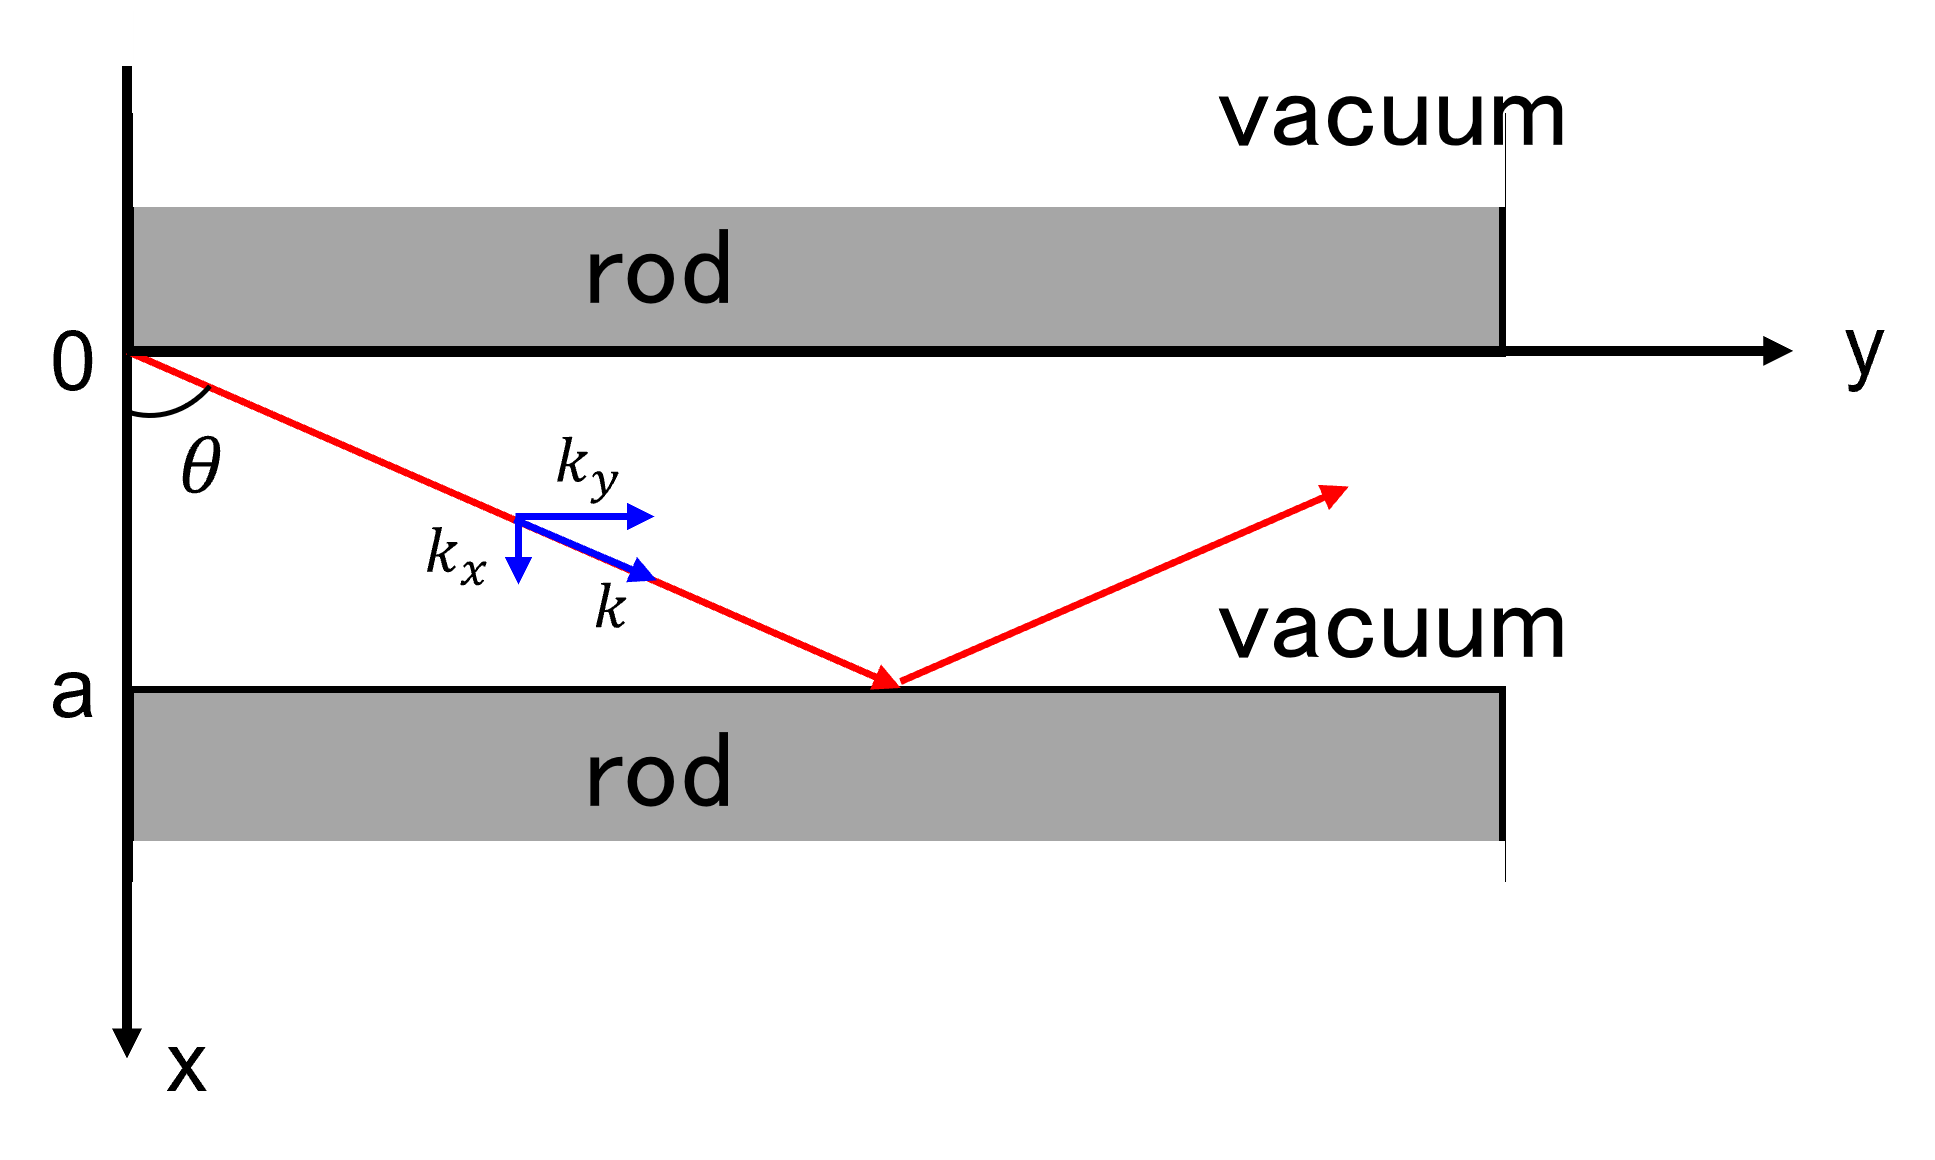
\includegraphics[scale=0.6]{./image/2-5/2-5_導波管.png}
      \caption{
        \label{fig:2-5_導波管}
        2枚の平行極板間の波動伝搬。$k$は入射した波動の波数である。
      }
    \end{center}
  \end{figure} 
  $x$軸と角$\theta$をなす$xy$平面内の波動は、$x=a$にある極板表面に到達した後、
  完全反射し$x$軸と$-\theta$の角をなして伝搬する。したがって、伝搬を表す指数因子は
  \begin{eqnarray}
    \label{eq:2-5-1}
    & e^{i[k(x \cos \theta + y \sin \theta ) - \omega_L t ] }  \nonumber \\
    & e^{i[k( - x \cos \theta + y \sin \theta ) - \omega_L t ] }
  \end{eqnarray}
  となる。ここで$k$は$k=2\pi/\lambda_0$($\lambda_0$:電磁波の波長)を満たす波数、$\omega_L$は角周波数である。このような波動には2つの偏波の可能性が考えられる。1つは電場$E$が$z$軸に平行な場合で、
  TE波(transverse electric wave)と呼ばれ、もう1つは磁場が$z$軸に平行な場合でTM(transverse magnetic wave)波と呼ばれる。
  以降に行うシミュレーションとの兼ね合いから、今回伝播する偏波はTM波であると仮定し、導出を行う。
  すなわち磁場は
  \begin{equation}
    \label{eq:2-5-2}
    \bm{B} = \bm{e_z} \left( B_1 e^{i[k(x \cos \theta + y \sin \theta ) - \omega_L t ] }
                  + B_2 e^{i[k(-x \cos \theta + y \sin \theta ) - \omega_L t ] }    \right)    
  \end{equation}
  と表す。ここで、磁場の境界条件より導体極板に平行な磁場$B_z$は境界面で0になることから、
  $x=0$で$B_z=0$となり、
  \begin{equation}
    \label{eq:2-5-3}
    B_1 = - B_2
  \end{equation}
  同様に$x=a$で$B_z=0$となるので、
  \begin{equation}
    \label{eq:2-5-4}
            B_1 e^{i[k(a \cos \theta + y \sin \theta ) - \omega_L t ] }
          - B_1 e^{i[k(-a \cos \theta + y \sin \theta ) - \omega_L t ] }    
          = 0 
  \end{equation}
  これを整理して
  \begin{equation}
    \label{eq:2-5-5}
    \left(  e^{ ika \cos \theta } - e^{ -ika \cos \theta } \right) e^{ i \left( ky \sin \theta - \omega_L t  \right) } 
          = 0 
  \end{equation}
  すなわち
  \begin{equation}
    \label{eq:2-5-6}
    ka \cos \theta = n \pi 
  \end{equation} 
  を満たす。したがって式(\ref{eq:2-5-2})は式(\ref{eq:2-5-6})を用いて
  \begin{eqnarray}
    \label{eq:2-5-7}
    B_x &=& 0  \\
    \label{eq:2-5-8}
    B_y &=& 0 \\
    \label{eq:2-5-9}
    B_z &=&  2 B_1 \cos ( \frac{n \pi}{a} x ) e^{ i \left( k_y y - \omega_L t  \right) }
  \end{eqnarray}
  ここで、$ \bm{\nabla} \times \bm{B} = - \frac{1}{c^2} \frac{\partial \bm{E} }{ \partial t } $ より、
  \begin{eqnarray}
    \label{eq:2-5-10}
    E_x &=& 2 B_1 \frac{c^2}{\omega_L} k_y \cos( \frac{n\pi}{a} x ) e^{ i \left( k_y y  - \omega_L t  \right) }  \\
    \label{eq:2-5-11}
    E_y &=& -2 i B_1  \frac{c^2}{\omega_L} \frac{n\pi}{a} \sin ( \frac{n \pi}{a} x ) e^{ i \left( k_y y - \omega_L t  \right) } \\
    \label{eq:2-5-12}
    E_z &=& 0
  \end{eqnarray}
  ただし、ここでは、波数の各方向の成分を$k_x = k \cos \theta $、$k_y = k \sin \theta $とする。
  式(\ref{eq:2-5-7})から(\ref{eq:2-5-12})は実空間において
  \begin{eqnarray}
    \label{eq:2-5-13}
    B_x &=& 0  \\
    \label{eq:2-5-14}
    B_y &=& 0 \\
    \label{eq:2-5-15}
    B_z &=&  2 B_1 \cos ( \frac{n \pi}{a} x ) \cos \left( k_y y - \omega_L t  \right) \\
    \label{eq:2-5-16}
    E_x &=& 2 B_1 \frac{c^2}{\omega_L} k_y \cos( \frac{n\pi}{a} x ) \cos \left( k_y y - \omega_L t  \right) \\
    \label{eq:2-5-17}
    E_y &=& -2 B_1  \frac{c^2}{\omega_L} \frac{n\pi}{a} \sin ( \frac{n \pi}{a} x ) \sin \left( k_y y - \omega_L t  \right) \\
    \label{eq:2-5-18}
    E_z &=& 0
  \end{eqnarray}
  と書き直すことができる。
  このとき、分散関係は
  \begin{equation}
    \label{eq:2-5-19}
    k^2 = k_x^2 + k_y^2
  \end{equation}
  であり、この条件の下で、式(\ref{eq:2-5-6})を満たす$\theta$を探すことで、伝搬可能な電磁波の波数(入射角度)が分かる。
  例えば、$n=1$のとき式(\ref{eq:2-5-6})は$\cos \theta = \lambda_0 / 2 a $となるが、$\lambda_0$が増すにつれて、
  分散関係を満たすために$k_y^2$は負でなければならない。
  このとき、(\ref{eq:2-5-7})~(\ref{eq:2-5-12})より、波は指数関数的に減衰してしまう。
  言い換えれば、$n = 1$における伝搬可能な最大の波長は$2a$であると言える。

  \subsection{反磁性電流}

流体の運動方程式は

\begin{eqnarray}
  \label{eq:2-6-1}
  mn \Biggl[ \frac{\partial \textit{\textbf{v}} }{\partial t} + (\textit{\textbf{v}}  \cdot \nabla ) \textit{\textbf{v}} \Biggr] = qn (\textit{\textbf{E}} + \textit{\textbf{v}} \times \textit{\textbf{B}}) - \nabla p
\end{eqnarray}

ここで、$\partial / \partial t = i \omega$  ととり$\textit{\textbf{v}}_\perp$のみ考えると、(1)左辺の第一項と(2)右辺の$qn (\textit{\textbf{E}} + \textit{\textbf{v}} \times \textit{\textbf{B}})$ との比は

\begin{eqnarray}
  \frac{(1)}{(2)} \approx \left| \frac{mni \omega v_\perp}{qnv_\perp B} \right| \approx \frac{\omega}{\omega _c}
\end{eqnarray}

$\omega _c$はサイクロン周波数。$\omega _c$の時間スケールに比べて遅いドリフトについては、(1)は無視できる。式(\ref*{eq:2-6-1})の右辺の$(\textit{\textbf{v}}  \cdot \nabla ) \textit{\textbf{v}} $ も無視できることは後述する。

よって式(\ref*{eq:2-6-1})は

\begin{eqnarray}
  0&=&qn (\textit{\textbf{E}} + \textit{\textbf{v}}_\perp \times \textit{\textbf{B}}) - \nabla p 
\end{eqnarray}

となり$\textit{\textbf{B}}$との外積をとると

\begin{eqnarray}
  0&=&qn (\textit{\textbf{E}} \times \textit{\textbf{B}} + (\textit{\textbf{v}}_\perp \times \textit{\textbf{B}}) \times \textit{\textbf{B}}) - \nabla p \times \textit{\textbf{B}} \nonumber \\
  0&=&qn (\textit{\textbf{E}} \times \textit{\textbf{B}} + \textit{\textbf{B}}(\textit{\textbf{v}}_\perp  \cdot \textit{\textbf{B}}) - \textit{\textbf{v}}_\perp B^2) - \nabla p \times \textit{\textbf{B}} \nonumber \\
  0&=&qn (\textit{\textbf{E}} \times \textit{\textbf{B}} +  - \textit{\textbf{v}}_\perp B^2) - \nabla p \times \textit{\textbf{B}} \nonumber \\
  qn \textit{\textbf{v}}_\perp B^2 &=& qn\textit{\textbf{E}} \times \textit{\textbf{B}} - \nabla p \times \textit{\textbf{B}}
\end{eqnarray}

したがって

\begin{eqnarray}
  \textit{\textbf{v}}_\perp &=& \frac{\textit{\textbf{E}} \times \textit{\textbf{B}}}{B^2} - \frac{\nabla p \times \textit{\textbf{B}}}{qn B^2} = \textit{\textbf{v}}_E + \textit{\textbf{v}}_D \\
  \label{eq:2-6-6}
  \textit{\textbf{v}}_E &=& \frac{\textit{\textbf{E}} \times \textit{\textbf{B}}}{B^2}\\
  \label{eq:2-6-7}
  \textit{\textbf{v}}_D &=& \frac{\nabla p \times \textit{\textbf{B}}}{qn B^2}
\end{eqnarray}

式(\ref{eq:2-6-6})は$\textit{\textbf{E}} \times \textit{\textbf{B}} $ドリフトで旋回中心のものと同じであるが、式(\ref{eq:2-6-7})は反磁性ドリフトと呼ばれるドリフトである。
$\textit{\textbf{v}}_D$は勾配の方向に対して垂直なので、先に$\textit{\textbf{v}}  \cdot \nabla \textit{\textbf{v}}$を無視したことが正当化される。それに伴う反磁性電流は、

\begin{eqnarray}
  \textit{\textbf{j}}_D = nq \textit{\textbf{v}}_{D}  = \frac{\nabla p \times \textit{\textbf{B}}}{B^2}
\end{eqnarray}

であり、圧力勾配があればいつでも電流$\textit{\textbf{j}}_D$が流れることを表す。
  \newpage 


%%%%%%%%%%%%%%%%%%%%%%%%%%%%%%%%%%%%%%%%% 3章 epic の概要 %%%%%%%%%%%%%%%%%%%%%%%%%%%%%%%%%%%%%%%%%%%%%%%%%%%%%%%%%%%%%%%%%%%%%%%%%%%%%%%%%%%%%%%%%%%%%%%%%%%
\section{粒子シミュレーションの基礎理論}
  \subsection{粒子コードEPIC3Dの概要と特徴}
  プラズマの運動を解析するには、現在流体モデルと運動論モデルの2種類の手法が存在する。
  前者は、局所的にプラズマが熱平衡状態であると仮定した上でMHD方程式を解くことにより巨視的振る舞いを観測するモデルである。
  これに対し、後者は荷電粒子によって生じる電磁場と各粒子にはたらく電磁場の力を計算し非平衡状態で起こる現象を再現するモデルである。
  このモデルでは、プラズマ振動数とデバイ長を空間ならびに時間を基準として使用するため、微小時間ごとのプラズマの微視的解析を行うことが可能である。
  しかし、粒子ごとに計算を行うため、粒子数や系の大きさ等に比例し必要な計算資源や計算時間が多くなるという欠点がある。
  これはPIC法と呼ばれる、多数の粒子の電荷と質量をまとめた超粒子という概念を想定することで補うことが可能である。
  ただこの概念を取り入れた場合においても、1000 以上もの超粒子を多体問題として扱うと膨大な量のクーロン力の計算が必要となる。
  そこでデバイ遮蔽というプラズマ特有の現象を利用し、計算量を削減する。デバイ長$\lambda_D$は
  \begin{equation}
    \label{3-1-1}
    \lambda_D = \sqrt{\frac{k_B T}{4\pi n e^2}}
  \end{equation}
  で表される。このデバイ長を半径に持つデバイ球外部では個々の荷電粒子により作り出される電場は
  他の荷電粒子が分極し遮蔽するので、値としては$\frac{1}{e}$以下となる。よって、デバイ球内部でのクーロン力の分布は
  プラズマの巨視的な振る舞いに関係せず、この場合は無視することが可能である。そのため、場については空間メッシュの格子点上でのみ定義することで
  Poisson方程式により計算する。デバイ遮蔽を再現するためには、空間メッシュをデバイ長と同程度にとる必要がある。
  そうすることで、粒子が受ける力とその力が起因となる運動も格子点上で与えられた電場から計算することが可能である。
  この一連の計算を繰り返すことで超粒子の概念の効果もあわせて計算量を大幅に減らすことが可能でありこれらを踏まえた方法でシミュレーションを実行した。

  \subsection{物理量の規格化}
  一般に長さや時間などの物理長には単位が存在するが、この単位を持つ物理量をそのまま用いてシミュレーションを行った場合、丸め誤差が増える恐れがある。\\
  そこで、数値シミュレーションでは物理量を、同じ次元のある値で割ることで、丸め誤差が増えることを避ける。
  このことを規格化という。この値は基礎方程式に従う必要がある。そこで、本研究では使用した各物理量を規格化した際の手順および規格化定数について記述する。
  また、各物理量の単位はCGS-Gauss 系である。\\
  \subsubsection{長さ}
  まず長さについて記述を行う。長さは系や媒質の大きさだけでなく、速度、密度などの次元に
  含まれる基本的な量である。シミュレーションで再現する実空間での長さを
  それぞれ$l_x,l_y,l_z$とする。これらは実空間の長さの次元を持つ。はじめに、
  これらの長さを$L_x,L_y,L_z$とし、計算機内における単位長さを

  \begin{equation}
    \label{eq:3-2-1}
    \Delta = \frac{l_x}{L_x}
  \end{equation}
  と定義する。シミュレーションにおけるパラメータ設定はx方向のスケールを基準に行われ、
  $l_x,L_x$を入力することで、それに基づいた$\Delta$が定まり、と同様に$l_y,l_z$を規格化することで
  計算機内での設定値$L_y,L_z$が算出される。その場合の$L_x,L_y,L_z$は
  \begin{equation}
    \label{eq:3-2-2}
    L_y=\frac{l_y}{\Delta}
  \end{equation}
  \begin{equation}
    \label{eq:3-2-3}
    L_z=\frac{l_z}{\Delta}
  \end{equation}
  の式によって計算される。\\
  \subsubsection{光速と時間}
  長さを規格化したので、次に長さの次元を含む光速を規格化したものを定義し、これによって時間の規格化を行う。
  そのために、まずは規格化されたプラズマ周波数$\tilde \omega_p$を求める。規格化された光速を$\tilde c$として、
  \begin{equation}
    \label{eq:3-2-4}
    \tilde \omega_p = \frac{c}{\tilde c}
  \end{equation}
  と表す。この場合、$\tilde c$ の値を決定する必要があり、本シミュレーションにおいて
  $\tilde c=10$として計算を行う。この規格化プラズマ周波数を用いれば規格化された時間
  $\tilde t$は
  \begin{equation}
    \label{eq:3-2-5}
    \tilde t=\frac{1}{\tilde \omega}
  \end{equation}
  と表される。また、と同様に規格化された粒子の速度は
  \begin{equation}
    \label{eq:3-2-6}
    \tilde v=\frac{v}{\Delta \omega_p}
  \end{equation}
  と表される。\\

  
  \subsubsection{質量と密度}
  次に質量と密度に関する規格化を行う。質量の規格化の基準として電子の質量を使用して
  \begin{equation}
    \label{eq:3-2-7}
    \tilde m=\frac{m}{m_e}
  \end{equation}
  と表す。また、プラズマ周波数$\omega_p$は
  \begin{equation}
    \label{eq:3-2-8}
    \omega_p=\sqrt{\frac{4\pi n e^2}{m}}
  \end{equation}
  であるから、この式を変形し、すでに求めた$\tilde m,\tilde \omega_p$を用いると
  \begin{equation}
    \label{eq:3-2-9}
    \tilde n= (\frac{\tilde m}{4\pi e^2})\tilde \omega_p
  \end{equation}
  となる。\\

  
  \subsubsection{電磁場}
  続いて電磁場の規格化について考える。これらはいずれも電子の運動方程式をもとに計算する。
  電子の電磁場中における運動方程式は
  \begin{equation}
    \label{eq:3-2-10}
    m \frac{d\bm{v}}{dt}=e(\textit{\textbf{E}}+
    \frac{\textit{\textbf{v}}}{c} \times \textit{\textbf{B}})
  \end{equation}
  であり、電荷の規格化因子を電子の電荷eで行った場合、規格化を考慮に入れると
  \begin{equation}
    \label{eq:3-2-11}
    m \frac{ d \widetilde{\bm{v}} }{ dt } 
    = e ( \widetilde{\bm{E}} + \frac{ \widetilde {\bm{v}} }{c} \times \bm{\widetilde {B}} )
  \end{equation}
  と表される。ここで(\ref{eq:3-2-10})のそれぞれの物理量の規格化の基準を$\bar m$のように表せば
  \begin{equation}
    \label{eq:3-2-12}
    {\bar m}{\tilde m}\frac{d(\Delta {\bar {\omega_p}} {\tilde v})}
    {d(\frac{1}{\bar {\omega_p}} \tilde t)}
    =e {\bar E} {\tilde E} + \frac{\Delta {\bar{\omega_p}}{\tilde v}}
    {\Delta {\bar{\omega_p}}{\tilde c}} \times e {\bar B}{\tilde B}
  \end{equation}
  となり、これを整理することで
  \begin{equation}
    \label{eq:3-2-13}
    \tilde{m} \frac{ d \tilde{v} }{ d \tilde{t} }
    = (\frac{e\bar E}{{\bar m} \Delta {\bar \omega_p}^2}){\tilde E} 
    + (\frac {e \bar{B} }{ \bar{m} \Delta \bar{\omega_p}^2}) 
    \frac{ \tilde{ \bm{v} } }{ \bm{c} } \times \tilde{ \bm{B} } 
  \end{equation}
  となる。(\ref{eq:3-2-11})、(\ref{eq:3-2-13})の$\tilde{\bm{E}}$ならびに
  $\tilde{\bm{B}}$の係数を比較すると電磁場の規格化定数は
  \begin{align}
    \label{eq:3-2-14}
    \bar E =&\frac{\bar m \Delta \bar \omega_p^2}{e}\\  
    \label{eq:3-2-15}
    \bar B =&\frac{\bar m \Delta \bar \omega_p^2}{e}  
  \end{align}
  となって、電場・磁場ともに等しくなる。さらに(\ref{eq:3-2-8})を変形した
  \begin{equation}
    \label{eq:3-2-16}
    \bar \omega_p^2 = \frac{4 \pi e^2 \bar n}{\bar m}
  \end{equation}
  この式を(\ref{eq:3-2-14})に代入することで
  \begin{equation}
    \label{eq:3-2-17}
    \bar E = \bar B = 4\pi e \Delta \bar n
  \end{equation}
  となる。これが電磁場の規格化となる。\\

  \subsubsection{レーザー強度}
  最後にレーザー強度の規格化について行う。電子の運動方程式(\ref{})は
  \begin{equation}
    \label{eq:3-2-18}
    \frac{dp}{dt}=-eE_0 \sin ( \omega t )  
  \end{equation}
  であり、初速0の初期条件の下でこれを解くと、運動量は
  \begin{equation}
    \label{eq:3-2-19}
    p=\frac{eE_0}{\omega} \cos (\omega t)
  \end{equation}
  ここで、この運動量の最大強度を電子の運動量$m_e c$で割った値を規格化強度$a_0$と定義する。
  \begin{equation}
    \label{eq:3-2-20}
    a_0 = \frac{e E_0}{m_e c \omega}
  \end{equation}
  これは、電子の速度が光速に近づくと$a_0$は1になることを表す。更に$E_0$について解き
  $\omega = \frac{2\pi c}{\lambda}$を代入することで
  \begin{equation}
    \label{eq:3-2-21}
    E_0 = \frac{2\pi a_0 mc^2}{e\lambda}
  \end{equation}
  が得られる。この式を(\ref{})に代入すると
  \begin{equation}
    \label{eq:3-2-22}
    I=\frac{c}{8\pi} \left(\frac{2\pi a_0 m c^2}{e\lambda}\right)^2 \times 10^{-7}
  \end{equation}
  となる。これが規格化されたレーザー強度である。これは$a_0$について解くと
  \begin{equation}
    \label{eq:3-2-23}
    a_0 = \left( \frac{2\times 10^7 e^2}{\pi m^2 c^5}\right) ^{\frac{1}{2}} I^{\frac{1}{2}}\lambda
  \end{equation}
  となる。


  \subsection{エネルギー保存則}
  粒子シミュレーションのような孤立系においては、エネルギー保存則を適用することができる。
  これは、シミュレーションが物理過程を正しく反映しているか確認するという観点から重要な式と言える。
  以下では、マクスウェル方程式よりエネルギー密度方程式を導出し、
  それを用いることでエネルギー保存則の導出を行う。

  マクスウェル方程式より、
  \begin{equation}
    \label{eq:3-3-1}
    \textit{\textbf{j}} = rot \textbf{\textit{H}} - \frac{\partial \textit{\textbf{D}} }{\partial t} 
  \end{equation}

  \begin{equation}
    \label{eq:3-3-2}
    rot \textit{\textbf{E}} = - \frac{\partial \textit{\textbf{B}} }{\partial t} 
  \end{equation}
  (\ref{eq:3-3-1})と(\ref{eq:3-3-2})にそれぞれ$\textbf{\textit{E}}$と$\textbf{\textit{B}}$との内積を取ると、
  \begin{equation}
    \label{eq:3-3-3}
    \textit{\textbf{E}} \cdot \textit{\textbf{j}} = \textit{\textbf{E}} \cdot rot \textit{\textbf{H}} - 
    \textit{\textbf{E}} \cdot \frac{\partial \textit{\textbf{D}} }{\partial t} - \textit{\textbf{H}} \cdot rot \textit{\textbf{E}}
    - \textit{\textbf{H}} \cdot \frac{\partial \textit{\textbf{B}} }{\partial t}
  \end{equation}
  $div( \textit{\textbf{E}} \times \textit{\textbf{H}} ) = 
  \textit{\textbf{H}} \cdot rot \textit{\textbf{E}} -
  \textit{\textbf{E}} \cdot rot \textit{\textbf{H}} $より、(\ref{eq:3-3-3})は
  \begin{equation}
    \label{eq:3-3-4}
    - \textit{\textbf{E}} \cdot \textit{\textbf{j}} =  
    \textit{\textbf{E}} \cdot \frac{\partial \textit{\textbf{D}} }{\partial t} 
    + \textit{\textbf{H}} \cdot \frac{\partial \textit{\textbf{B}} }{\partial t}
    + div( \textit{\textbf{E}} \times \textit{\textbf{H}} )
  \end{equation}
  と変形できる。ここで、右辺の第1項、第2項について電磁波のエネルギーを$U_F$とすると
  \begin{equation}
    \label{eq:3-3-5}  
    \textit{\textbf{E}} \cdot \frac{\partial \textit{\textbf{D}} }{\partial t} 
    + \textit{\textbf{H}} \cdot \frac{\partial \textit{\textbf{B}} }{\partial t} =
    \frac{\partial}{\partial t } (\frac{1}{2}\epsilon_0 E^2 + \frac{1}{2} \mu_0 H^2) =
    \frac{\partial U_F }{\partial t } 
  \end{equation}
  ポインティングベクトルを
  \begin{equation}
    \label{eq:3-3-6}
    \textit{\textbf{S}} = \textit{\textbf{E}} \times \textit{\textbf{H}} 
  \end{equation}
  をすると(\ref{eq:3-3-4})は結局
  \begin{equation}
    \label{eq:3-3-7}
    - \textit{\textbf{E}} \cdot \textit{\textbf{j}} =  
    \frac{\partial U_F }{\partial t }    
    + \bm{\nabla} \cdot \textit{\textbf{S}} 
  \end{equation}
  と書き直すことができる。
  この式をエネルギー密度方程式と呼ぶ。
  系の体積を$V$として体積平均を考えると
  \begin{equation}
    \label{eq:3-3-8}
     - \frac{1}{V} \int_V \textit{\textbf{E}} \cdot \textit{\textbf{j}} \: d\bm{V} 
     = \frac{1}{V} \int_V \frac{\partial U_F }{\partial t } \: d\bm{V}
     + \frac{1}{V} \int_V \bm{\nabla} \cdot \textit{\textbf{S}} \: d\bm{V}
  \end{equation}
%   ここで電流$\bm{j}$を粒子系の電流$\bm{j}_p$と、系内に入力するアンテナ電流$\bm{j}_a$に分けて
%   \begin{equation}
%     \label{eq:31}
%     \bm{j} = \bm{j}_p + \bm{j}_a 
%   \end{equation}
%   特に粒子系の電流について
  ただし、ここで電流$\bm{j}$を粒子系の電流$\bm{j}_p$と外部から入力するアンテナ電流$\bm{j}_\alpha$に分けると、
  粒子系の電流について
  \begin{equation}
    \label{eq:3-3-9}
    \bm{j_p} = \Sigma_\sigma \Sigma_j^{N_\sigma} q_{\sigma j} \bm{v}_{\sigma j}\delta(\bm{r}-\bm{r}_{\sigma j})
  \end{equation}
  ここで$\sigma$は粒子種、$N$は粒子数、$q$は粒子の電荷、$v$は粒子の速度である。
  また、粒子の従う運動方程式(\ref{eq:2-})より、外部磁場の存在しない系において、エネルギー方程式は
  \begin{equation}
    \label{eq:3-3-10}
      \frac{\partial}{\partial t} \Sigma_\sigma \Sigma_j^{N_\sigma} ( \bm{r}_{\sigma j} m_{\sigma j} c^2 ) 
      = \Sigma_\sigma \Sigma_j^{N_\sigma} q_{\sigma j} \bm{v}_{\sigma j} \bm{E}(\bm{r}_{\sigma j})
  \end{equation}
  このとき、
  \begin{align}
    \label{eq:3-3-11}
    \nonumber
    \int_V \bm{E} \cdot \bm{j_p} \: d\bm{V}  &= \int_V \Sigma_\sigma \Sigma_j^{N_\sigma} q_{\sigma j} \bm{v}_{\sigma j}\delta(\bm{r}-\bm{r}_{\sigma j}) \bm{E}(\bm{r}_{\sigma j})\: d\bm{V} \\
    \nonumber
          &= \Sigma_\sigma \Sigma_j^{N_\sigma} q_{\sigma j} \bm{v}_{\sigma j} \bm{E}(\bm{r}_{\sigma j})  \\
    &= \frac{\partial}{\partial t} \Sigma_\sigma \Sigma_j^{N_\sigma} ( \bm{r}_{\sigma j} m_{\sigma j} c^2 )
  \end{align}
  すなわち、(\ref{eq:3-3-8})は
  \begin{equation}
    \label{eq:3-3-12}
    - \frac{\partial}{\partial t} \left( \frac{1}{V} \Sigma_\sigma \Sigma_j^{N_\sigma} ( \bm{r}_{\sigma j} m_{\sigma j} c^2 ) 
    + \frac{1}{V} \int_V U_F \: d\bm{r}  \right) - \frac{1}{V} \int_V \bm{E} \cdot \bm{j_\alpha} \: d\bm{r} 
    = \frac{1}{V} \int_V \bm{\nabla} \cdot \bm{S} \: d\bm{V}
  \end{equation}
  左辺第1項は、まさに全粒子の運動エネルギーそのものを表しており、電子とイオンで分けると
  \begin{equation}
    \label{eq:3-3-13}
      \ev{U_K} = \frac{1}{V} \Sigma_\sigma \Sigma_j^{N_\sigma} ( \bm{r}_{\sigma j} m_{\sigma j} c^2 )
      = \ev{U_{Ki}} + \ev{U_{Ke}} 
  \end{equation}
  また、同様に各項をブラケット表記で表すと、電磁場のエネルギーは
  \begin{equation}
    \label{eq:3-3-14}
     \ev{U_F} = \frac{1}{V} \int_V U_F \: d\bm{r}
  \end{equation}
  系内に入力するアンテナエネルギーは
  \begin{equation}
    \label{eq:3-3-15}
     \ev{W_A} = - \frac{1}{V} \int_V \bm{E} \cdot \bm{j_\alpha} \: d\bm{r}
  \end{equation}
  系外に流出するポインティングエネルギーは
  \begin{align}
    \label{eq:3-3-16}
    \nonumber
      \ev{W_P} &= \frac{1}{V} \int_V \bm{\nabla} \cdot \bm{S} \: d\bm{V} \\
      &= \frac{1}{V} \int_D \bm{S} \cdot \bm{n} \: dD
  \end{align}
  ただし、ここでガウスの発散定理を用いた。$\bm{n}$は閉局面$D$に垂直な単位法線ベクトルである。
  まとめると、(\ref{eq:3-3-12})式は結局
  \begin{equation}
    \label{eq:3-3-17}
    - \frac{\partial}{\partial t} \left( \ev{U_K} + \ev{U_F} \right) + \ev{W_A} = \ev{W_P}
  \end{equation}
  と書き表すことが出来る。(\ref{eq:3-3-17})をシミュレーション終端時間まで積分するとエネルギー保存則は以下のように定まる。
  \begin{equation}
    \label{eq:3-3-18}
      \left( \ev{U_K(t)} - \ev{U_K(0)} 
      +  \ev{U_F(t)} - \ev{U_F(0)} \right) - \int_0^t \ev{W_A} \: dt 
      = - \int_0^t \ev{W_P} \: dt
  \end{equation}

  EPIC3Dでは、シミュレーション空間の境界端に、アンテナエネルギーを球面波として入力しており、
  そのうちの半分は物質と相互作用することなく系外へと抜けていく。(\ref{eq:3-3-18})を以下のように変形する。
  \begin{equation}
    \label{eq:3-3-19}
      \left( \ev{U_K(t)} - \ev{U_K(0)} 
      +  \ev{U_F(t)} - \ev{U_F(0)} \right) - \frac{1}{2} \int_0^t \ev{W_A} \: dt 
      = - \int_0^t \ev{W_P} \: dt + \frac{1}{2} \int_0^t \ev{W_A} \: dt
  \end{equation}
  左辺の$\frac{1}{2} \int_0^t \ev{W_A} \: dt$は
  系内に入力される実効的なアンテナエネルギーを示しており、右辺は実効的なポインティングエネルギーである。
ここで、相対誤差は
\begin{equation}
  \label{eq:3-3-20}
    \frac{ \left( \ev{U_K(t)} - \ev{U_K(0)} 
    +  \ev{U_F(t)} - \ev{U_F(0)} \right) - \frac{1}{2} \int_0^t \ev{W_A} \: dt 
    + \int_0^t \ev{W_P} \: dt - \frac{1}{2} \int_0^t \ev{W_A} \: dt }
    { \frac{1}{2} \int_0^t \ev{W_A} \: dt + \ev{U_K(0)} + \ev{U_F(0)} }
\end{equation}
のように表され、シミュレーションで見られた物理現象の正当性を確かめる1つの指標となる。

\newpage
  

%%%%%%%%%%%%%%%%%%%%%%%%%%%%%%%%%%%%%%%%% 4章 シミュレーションの結果 %%%%%%%%%%%%%%%%%%%%%%%%%%%%%%%%%%%%%%%%%%%%%%%%%%%%%%%%%%%%%%%%%%%%%%%%%%%%%%%%%%%%%%%%%%%%%%%%%%%
\section{高強度レーザーと構造性ターゲットの相互作用シミュレーション}

\subsection{スラブターゲットへの照射}
高強度レーザーと構造性媒質との相互作用を調べるためには、単純な媒質を用いた場合と比較して検討することが重要である。したがって、ここでは単純な媒質であるスラブターゲットに高強度レーザーを照射したシミュレーションについて述べる。

\subsubsection{シミュレーション条件}
シミュレーションは図1 に示す通り、x 方向のシステムサイズ Lx = 20.48µm、y 方向のシステムサイズ Ly = 15.36µm の長方形の領域を設定し、y方向の10$\sim$12µmの範囲にスラブターゲットを配置した。

\begin{figure}[H]
  \begin{center}
    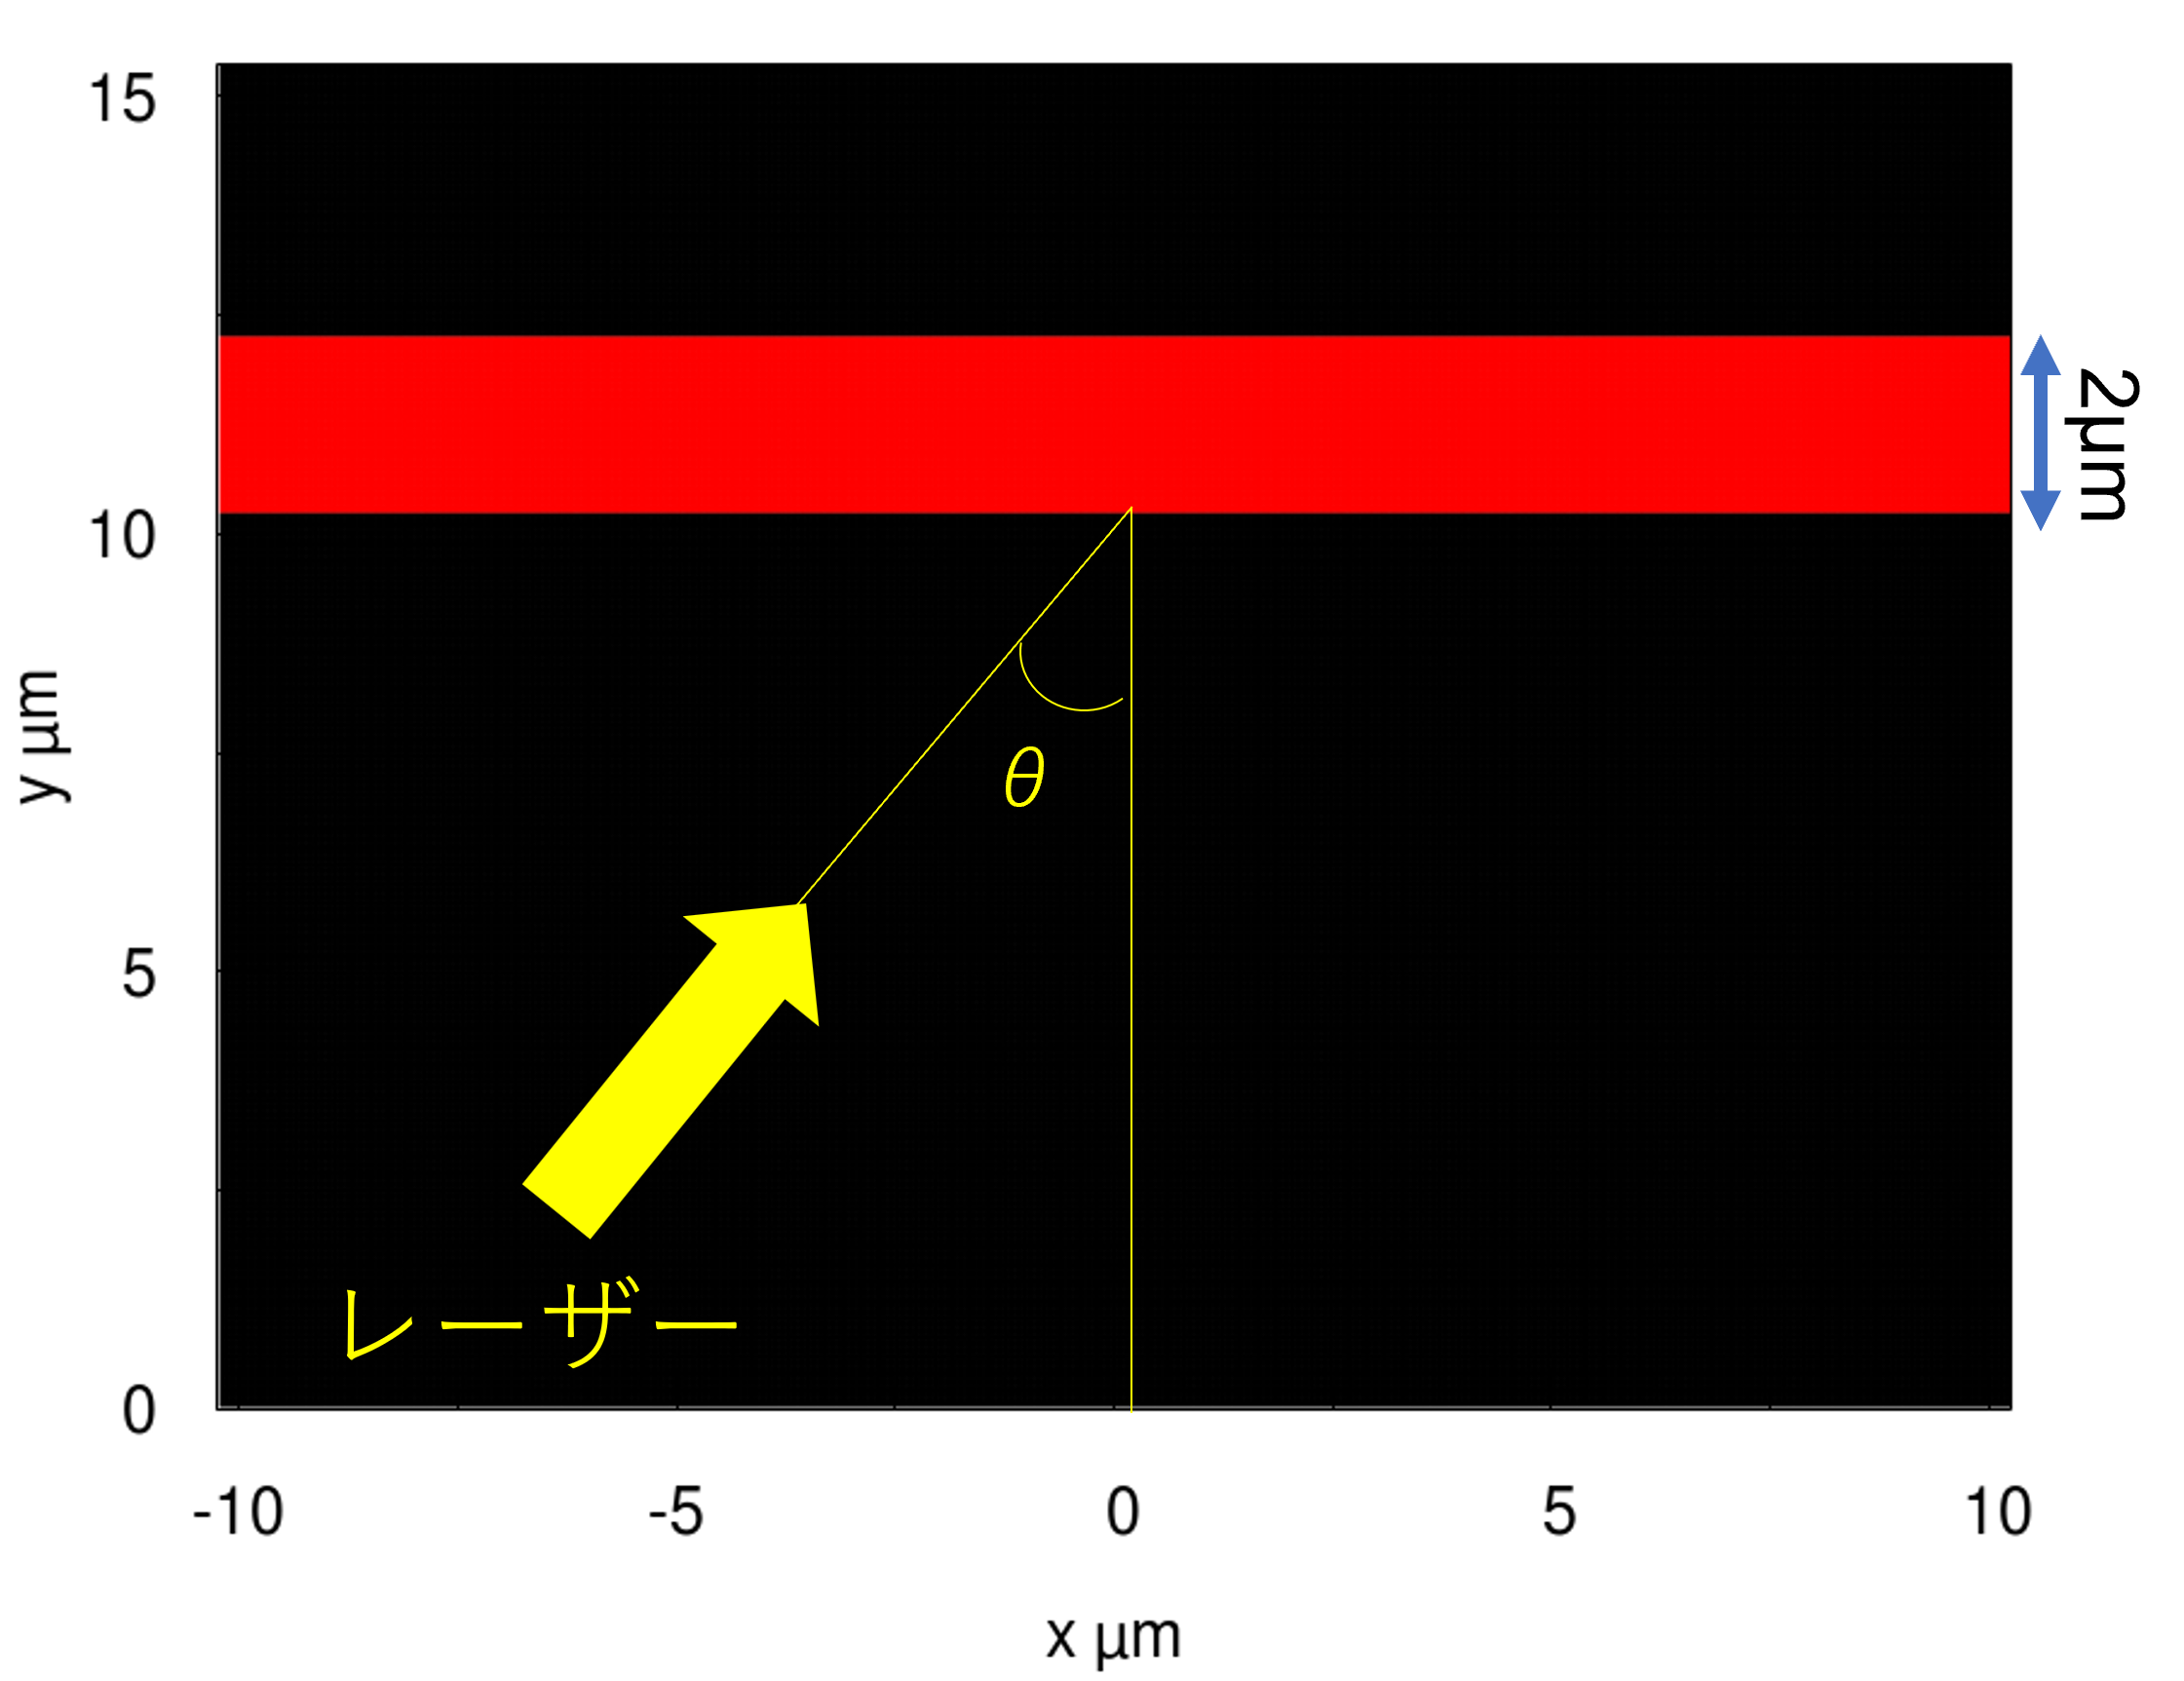
\includegraphics[scale=0.4]{./image/4-1-slab.png}
    \label{fig:4-1}
    \caption{スラブターゲットの図}
  \end{center}
\end{figure}

この系に対して、パルス幅が 40 fs(FWHM)、最大集光強度が$1.2×10^{19}W/cm^2$に達する高強
度レーザーを +y方向から$\theta=$30度の角度で照射した。ここで、レーザーは y=40 nm に設置したアンテナから誘導電流を流すことにより発振させており、粒子 (電子とイオン)・場 (電場・磁場) ともに、xy 方向に透過(吸収)境界条件を課している。詳細なシミュレーション条件は表 2 に示す。

\begin{table}[H]
  \begin{center}
    \caption{シミュレーション設定}
  \begin{tabular}{|l|r|} \hline
    \multicolumn{2}{|c|}{レーザー条件} \\ \hline
    レーザー強度 & $\textit{I}=1.2\times  10^{19}[W/cm^2]$ \\ 
    規格化強度 & $\textit{a} _0 = 2.39$ \\
    パルス幅 & 40fsec \\ 
    レーザープロファイル(波形)[時間方向] & ガウシアン \\
    レーザー空間分布 & 平面波 \\
    カットオフ密度 & $\textit{n} _c = 1.7 \time 10^21 [cm^{-3}]$ \\\hline
    \multicolumn{2}{|c|}{ターゲット条件} \\ \hline
    イオンの種類 & ケイ素(Si) \\
    電子密度 &$6.98 \times  10 ^{23} [\rm{cm}^{-3}]$ \\\hline
    \multicolumn{2}{|c|}{系} \\ \hline
    システムサイズ(x方向) & [20.48$\mu $m] \\
    システムサイズ(y方向) & [15.36$\mu $m] \\
    メッシュ数(x方向) & [1024] \\
    メッシュ数(y方向) & [768] \\
    メッシュ幅(x方向) & [20nm] \\
    メッシュ幅(y方向) & [20nm] \\
    時間幅 & $1/6$[fs] \\ \hline
    \multicolumn{2}{|c|}{境界条件} \\ \hline
    粒子(x方向) & 周期 \\
    粒子(y方向) & 透過 \\
    電磁波(x方向) & 周期 \\
    電磁波(y方向) & 透過 \\ \hline
  \end{tabular}
  \end{center}
  \end{table}

  \subsubsection{エネルギーダイナミクス}
はじめに、系のエネルギーダイナミクスを示す。横軸は時間、縦軸は規格化したエネルギーを表している。

\begin{figure}[H]
  \begin{center}
    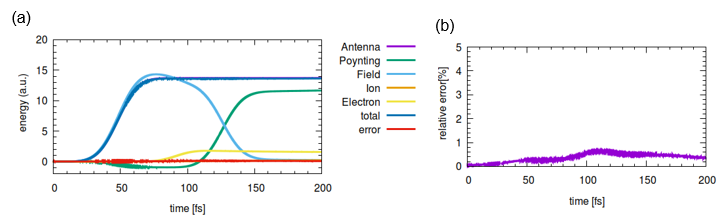
\includegraphics[scale=0.5]{./image/4-2-slab_dynamics.png}
    \label{fig:4-2}
    \caption{シミュレーション範囲内のエネルギーに関する時間発展図。(a)はアンテナからシステムに入ったエネルギー(Antenna)を紫色、システムから外部に抜け出たエネルギー(Poynting)を緑色、システム内の電磁エネルギー(Field : 電場のエネルギー$\epsilon_0E^{2}/2 +$磁場のエネルギー$B^{2}/2\mu_0$)を水色、イオンによるエネルギー(Ion)を橙色、電子によるエネルギー(Electron)を黄色、合計のエネルギー(total)を赤色で表している。(b)は合計のエネルギー(total)とシステムから外部に抜け出たエネルギー(poynting)の差である相対誤差を表している。}
  \end{center}
\end{figure}
%$𝜀_0E^2/2$ $B^2/2𝜇_0$

Antenna(紫色)は、レーザーのエネルギーであり、全体のエネルギー(total、青色)は、場のエネルギー(Field、水色)、電子(Electron、黄色)、イオン(Ion、橙色)のエネルギーを足し合わせた値である。また、poynting は系から抜けだしていくエネルギー(緑色)を表している。まず、レーザーが照射された後、80fs付近から質量の軽い電子はレーザーからエネルギーを得て加速している。120fs 付近で照射したレーザーがターゲットに反射され系を通り抜け始めるので、poynting の値が大きくなる。その後約 180fs から全ての値が、ほぼ一定になる。また、(b)を見ると、相対誤差は 1%以下になっており、誤差は許容される範囲にあると考えられる。

\subsubsection{密度の2次元空間分布}

電子とイオンそれぞれの密度分布を示す。

\begin{figure}[H]
  \begin{center}
    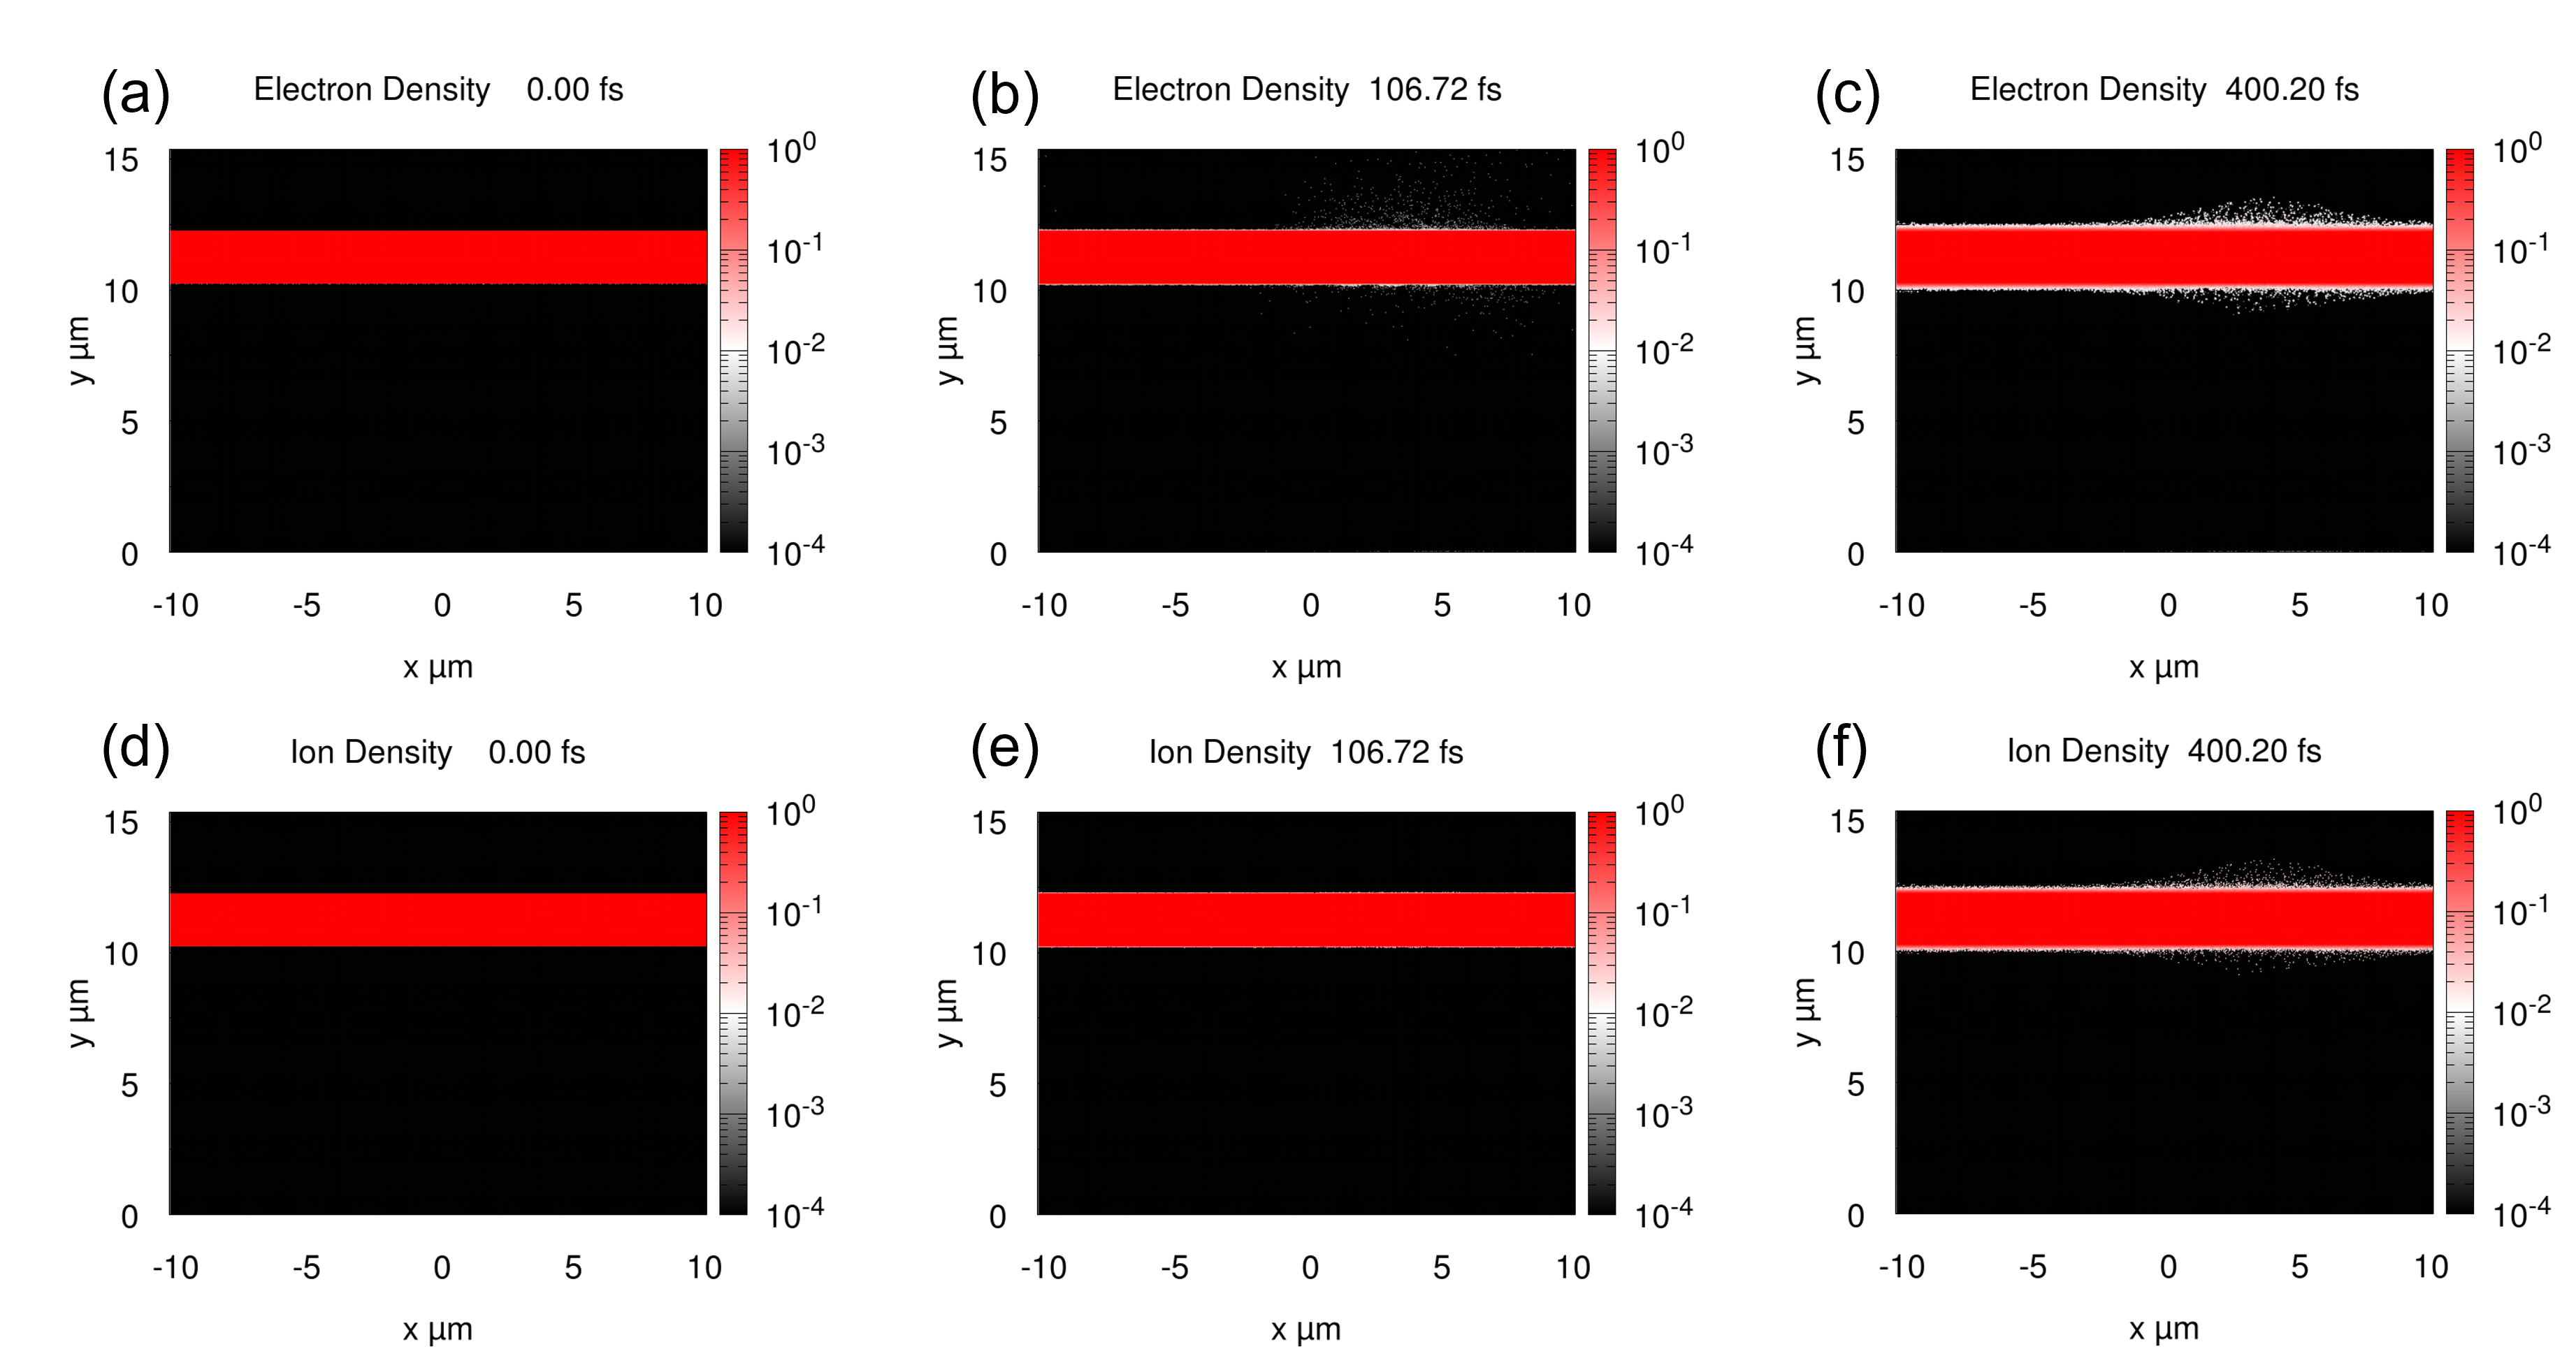
\includegraphics[scale=0.5]{./image/4-5-slab_density.png}
    \label{fig:4-3}
    \caption{シミュレーション範囲内の電子とイオンの密度分布図。初期値の値で規格化している。シミュレーション開始時刻をt=0としている。(a)-(c)はそれぞれ時刻t=0fs, 106.67fs, 86.67fsの場合の電子の密度分布、(d)-(f)はそれぞれ時刻t=0fs, 106.67fs, 86.67fsの場合のイオンの密度分布表している。}
  \end{center}
\end{figure}

図は電子とイオンの密度分布を表している。(a),(d)は初期分布を表している。(b)はレーザーがターゲットに当たり質量の軽い電子がポンデロモーティブ力によりレーザーの進行方向に加速されることによって密度部分布が膨張している。一方で(e)は質量が大きいイオンは動かに状態にある。その後、(c),(f)からわかるように400.20fs では、電子、イオン共に系全体に広がっていることが分かる。

\subsubsection{磁場の2次元空間分布}

ターゲットにレーザーを照射したときの様子を表すためにz方向の磁場Bzを示す。

\begin{figure}[H]
  \begin{center}
    \includegraphics[scale=0.5]{./image/4-4-slab_Bz.png}
    \label{fig:4-4}
    \caption{シミュレーション範囲内のz方向の磁場Bzの図。シミュレーション開始時刻をt=0としている。(a)-(f)はそれぞれ時刻t=26.67fs, 66.67fs, 86.67fs, 106.67fs, 140.00fs, 400.00fsの場合を表している。カラーマップはz方向の磁場Bzを-10~10kTで表している。}
  \end{center}
\end{figure}
図4.3はレーザーが照射されている様子を表している。(a),(b)はレーザーが図の左下からレーザーが照射されているフェーズである。(c),(d)はレーザーがターゲットに当たり反射されているフェーズであり、その際に電子がレーザー照射方向にポンデロモーティブ力によって加速されることによって磁場が形成されている。(e),(f)はレーザーがターゲットに反射されてた後の磁場の様子を表している。(f)からもわかるようにレーザーが照射されてからターゲットに反射してしばらくたった時間では、強い磁場は残っていないことがわかり、プラズマを制御するにたる磁場強度は生成できていない。

\subsubsection{電磁場エネルギーの時間発展}
スラブターゲットにレーザーが照射された際のシュミレーション範囲内の電磁場エネルギーの時間発展を示す。

\begin{figure}[H]
  \begin{center}
    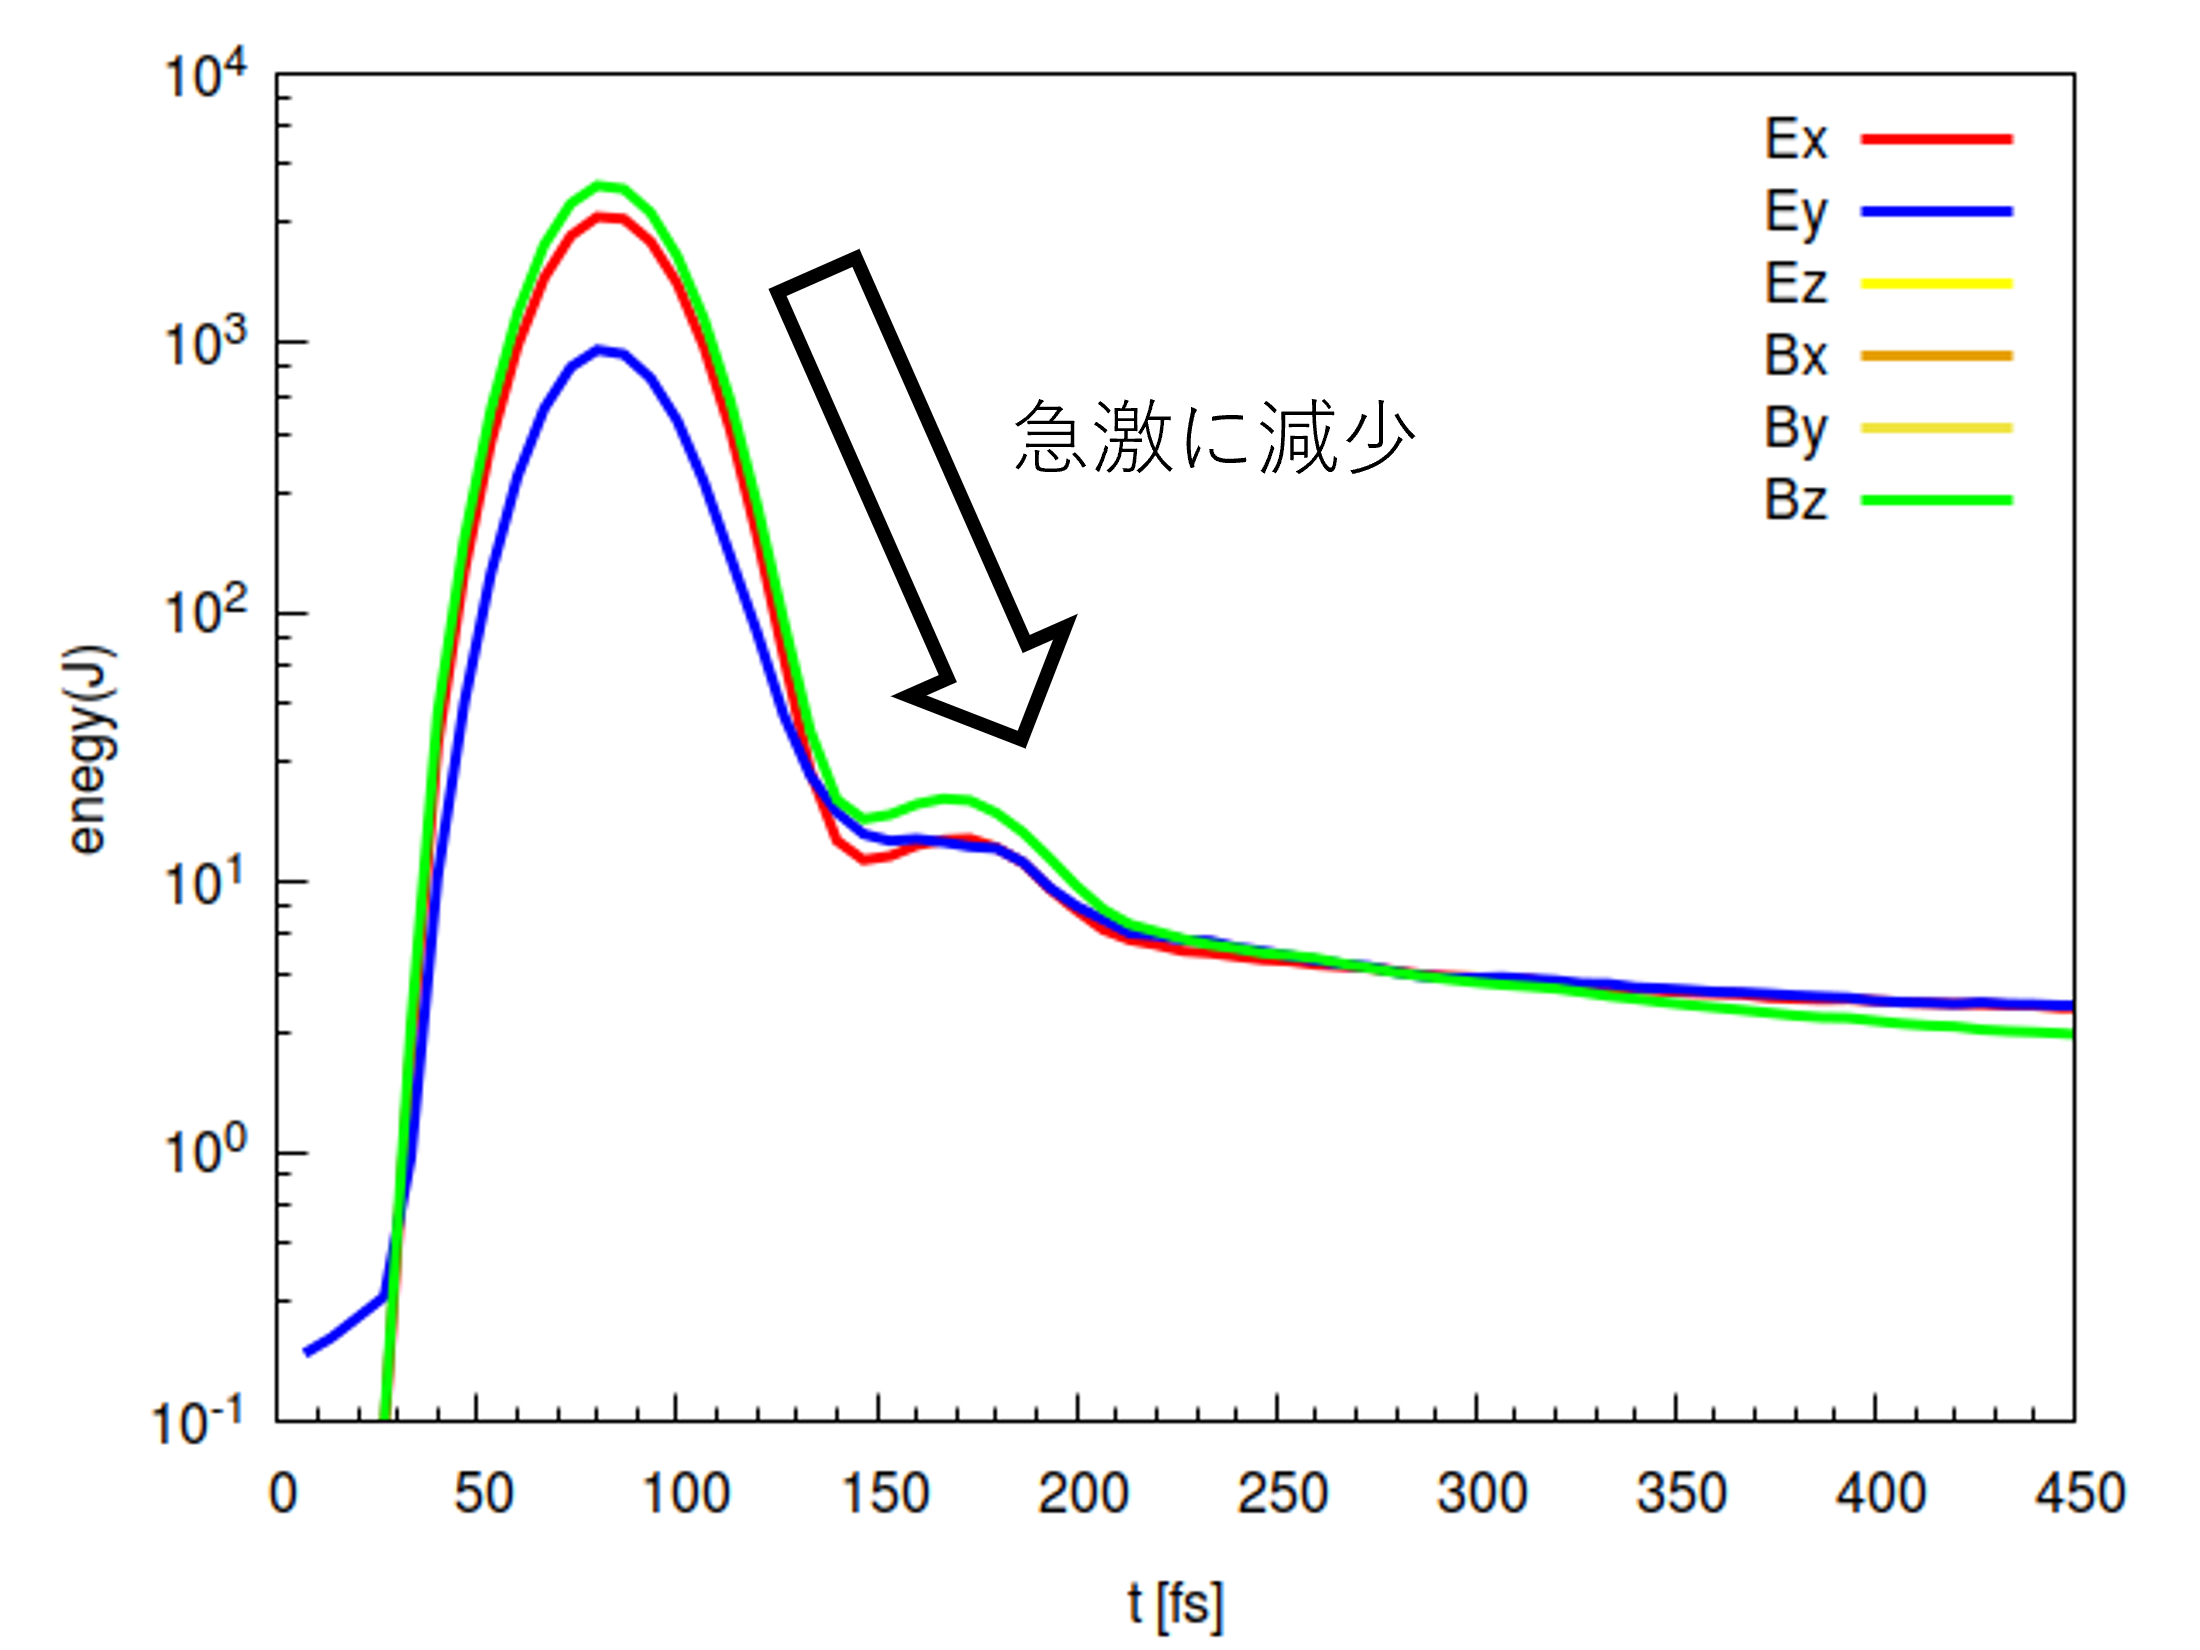
\includegraphics[scale=0.5]{./image/4-15-slab.png}
    \label{fig:4-4-2}
    \caption{シュミレーション範囲内の電磁場エネルギーの時間発展}
  \end{center}
\end{figure}

シュミレーション範囲内の電磁場エネルギーの時間発展の図。赤色はEx,青色はEy,緑色はBzのエネルギーを表している。
図からわかるようにfs付近でレーザー場によって各電磁場エネルギーは増加するが、fs付近で急激に減少していき、プラズマをレーザーのパルス時間オーダーよりも長く制御できるほどの電磁場は発生していないことがわかる。したがってこの単純なターゲットではプラズマをレーザーのパルス時間オーダーよいも長く制御することはできない。

\subsection{2本のロッドターゲットへの照射}
前節では、単純な媒質でであるスラブターゲットを用いたが、プラズマを閉じ込めうる磁場は保持されなかった。先行研究でµmオーダーの微細構造をターゲットに付与することで、レーザーのパルス時間を越えた準定常な強磁場生成等の単純な媒質では見られない現象をシミュレーションによって見出している。そこでここでは、前節のスラブターゲットにµmオーダーの2本のロッドをを加えたターゲットを用いて、準定常な磁場生成やその時の電流路について述べる。

\subsubsection{シミュレーション条件}
シミュレーションは図 に示す通り、x 方向のシステムサイズ Lx = 20.48μm、y 方向のシステムサイズ Ly = 15.36μm の長方形の領域を設定し、y 方向の 10~12μm の範囲にスラブターゲットと2本のロッド径が0.5μmのロッドを配置した。

\begin{figure}[H]
  \begin{center}
    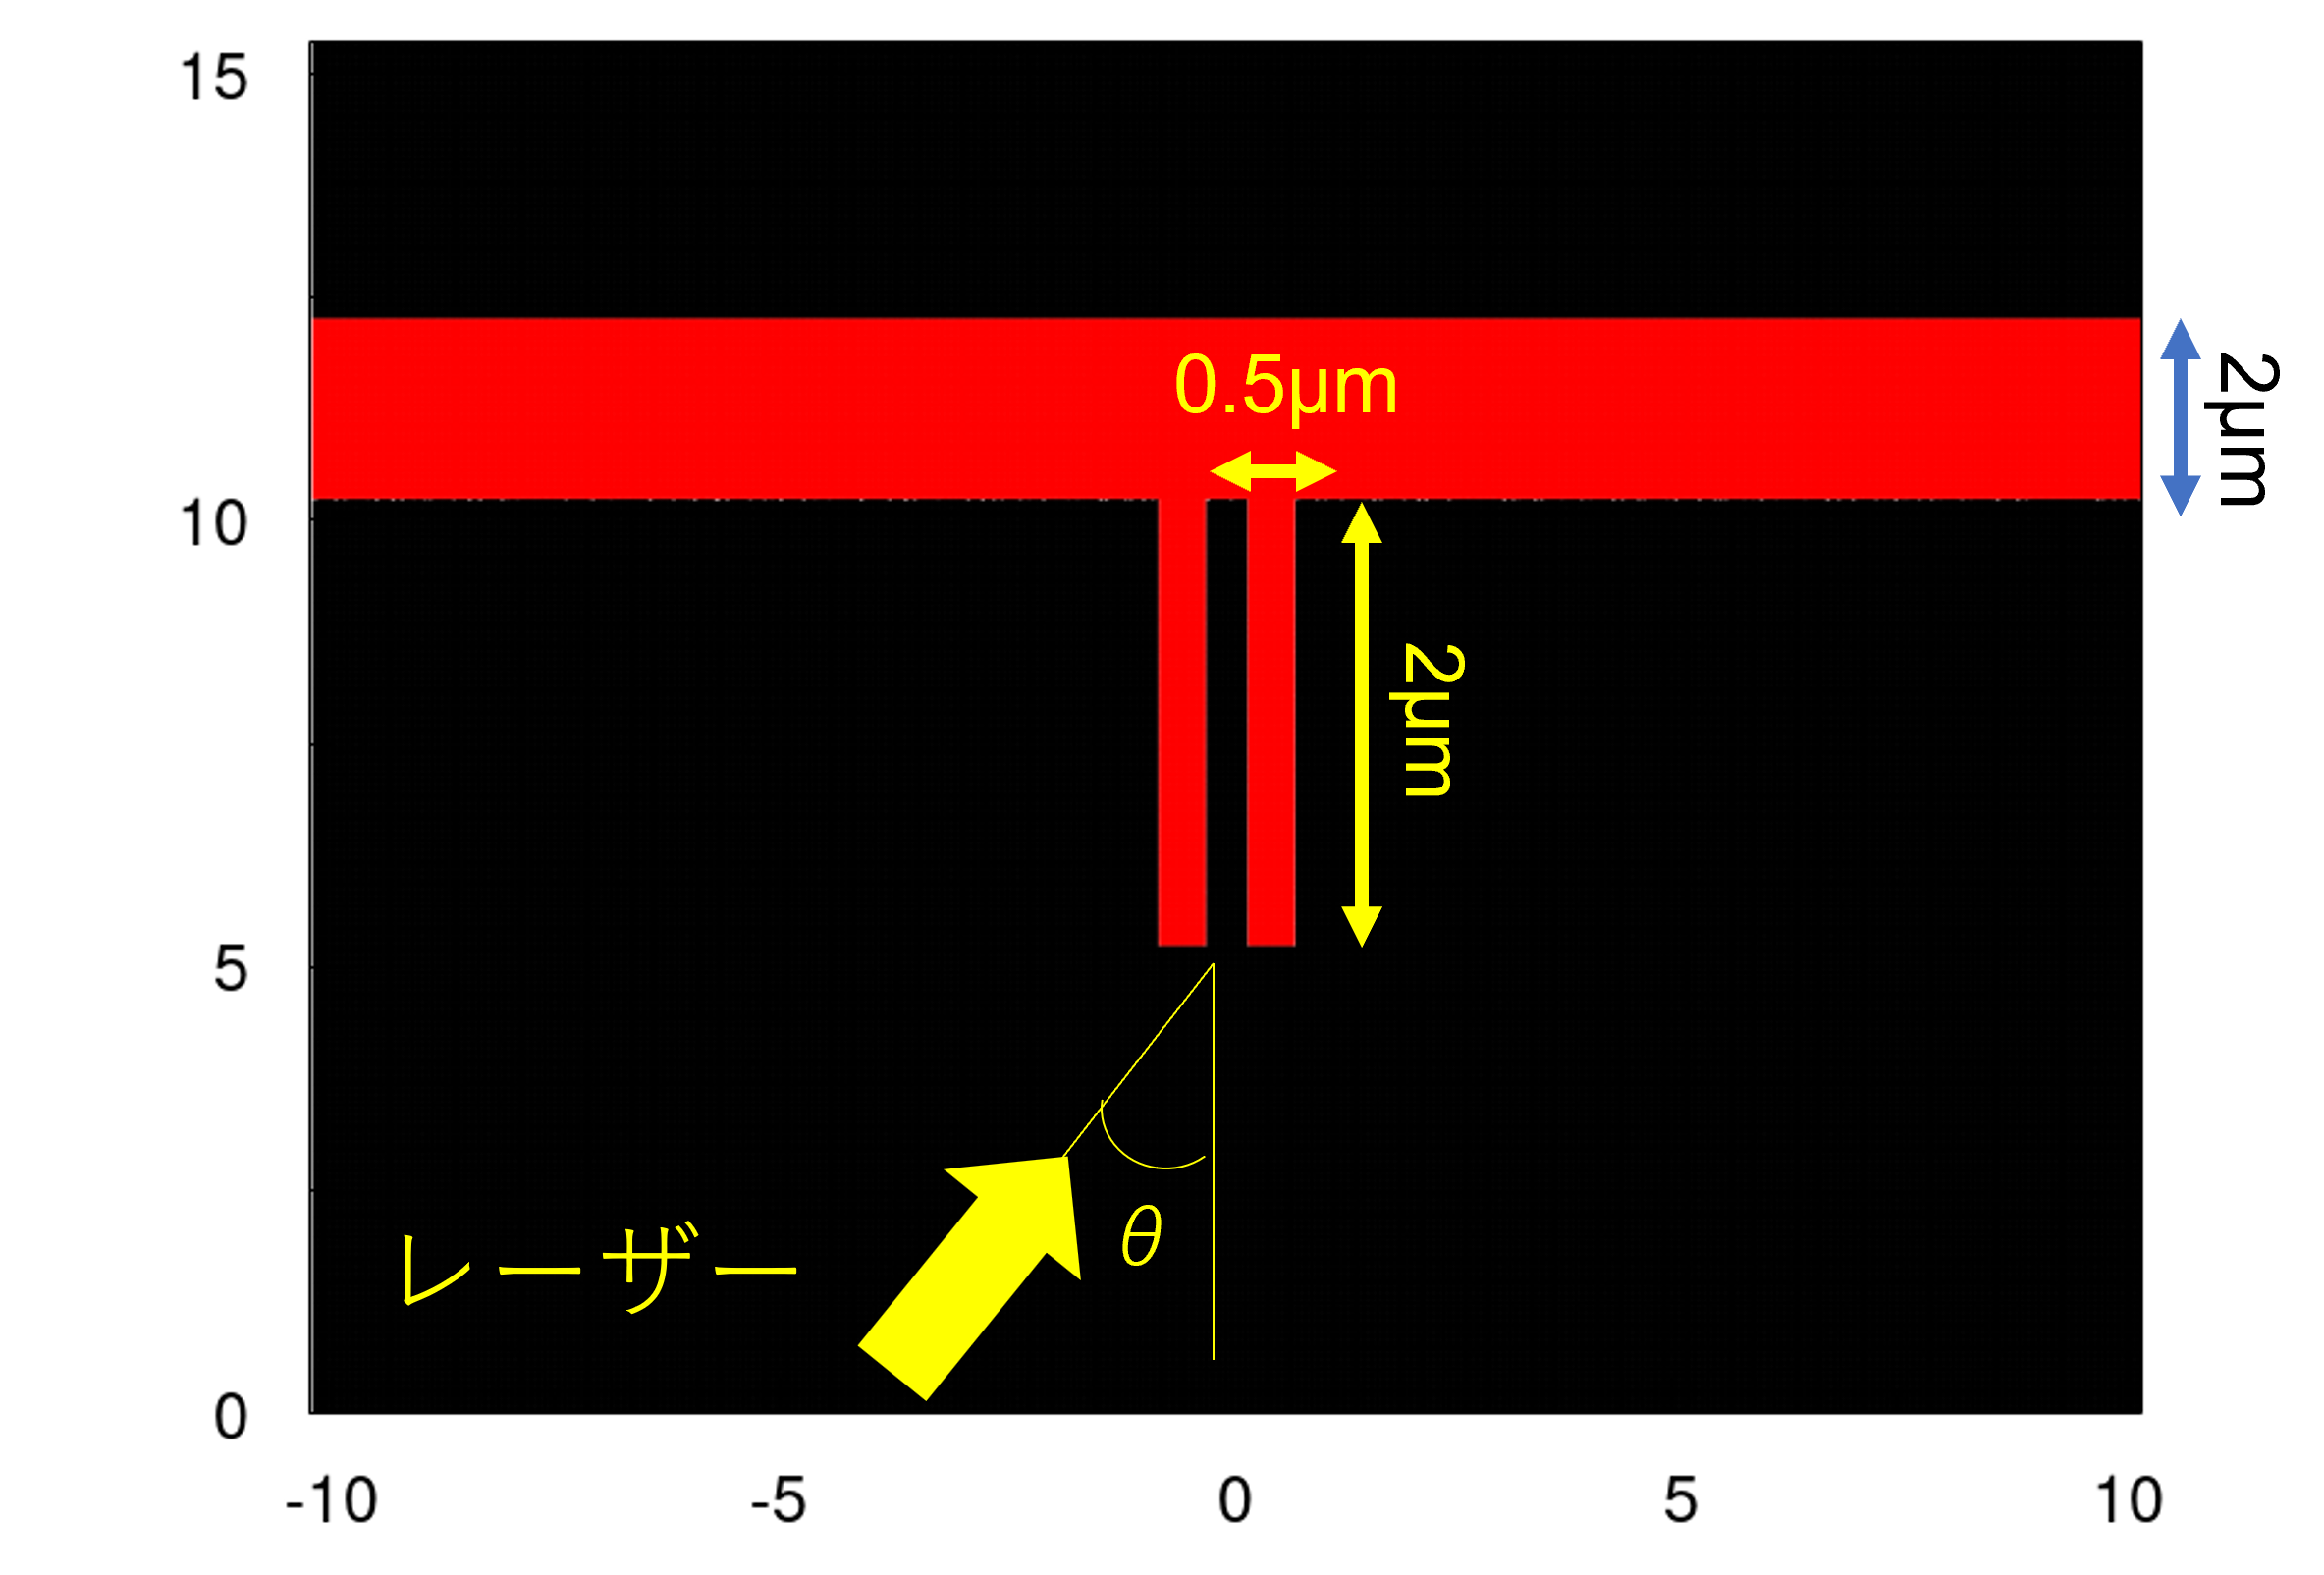
\includegraphics[scale=0.4]{./image/4-6-2rod.png}
    \label{fig:4-5}
    \caption{スラブターゲットと2本ロッドの図}
  \end{center}
\end{figure}

この系に対して、スラブターゲットに照射したレーザーと同様のパルス幅が 40 fs(FWHM)、最大集光強度が$1.2×10^{19}W/cm^2$に達する高強度レーザーを +y方向から$\theta=$30度の角度で照射した。ここで、レーザーは y=40 nm に設置したアンテナから誘導電流を流すことにより発振させており、粒子 (電子とイオン)・場 (電場・磁場) ともに、xy 方向に透過(吸収)境界条件を課している。詳細なシミュレーション条件は表に示す。


\begin{table}[H]
  \begin{center}
    \caption{シミュレーション設定}
  \begin{tabular}{|l|r|} \hline
    \multicolumn{2}{|c|}{レーザー条件} \\ \hline
    レーザー強度 & $\textit{I}=1.2\times  10^{19}[W/cm^2]$ \\ 
    規格化強度 & $\textit{a} _0 = 2.39$ \\
    パルス幅 & 40fsec \\ 
    レーザープロファイル(波形)[時間方向] & ガウシアン \\
    レーザー空間分布 & 平面波 \\
    カットオフ密度 & $\textit{n} _c = 1.7 \time 10^21 [cm^{-3}]$ \\\hline
    \multicolumn{2}{|c|}{ターゲット条件} \\ \hline
    イオンの種類 & ケイ素(Si) \\
    電子密度 &$6.98 \times  10 ^{23} [\rm{cm}^{-3}]$ \\
    ロッド直径 & 0.5[$\mu$ m] \\
    ロッドの長さ & 10[$\mu$ m] \\
    ロッドの本数 & 2本 \\ \hline
    \multicolumn{2}{|c|}{系} \\ \hline
    システムサイズ(x方向) & [20.48$\mu $m] \\
    システムサイズ(y方向) & [15.36$\mu $m] \\
    メッシュ数(x方向) & [1024] \\
    メッシュ数(y方向) & [768] \\
    メッシュ幅(x方向) & [20nm] \\
    メッシュ幅(y方向) & [20nm] \\
    時間幅 & $1/6$[fs] \\ \hline
    \multicolumn{2}{|c|}{境界条件} \\ \hline
    粒子(x方向) & 周期 \\
    粒子(y方向) & 透過 \\
    電磁波(x方向) & 周期 \\
    電磁波(y方向) & 透過 \\ \hline
  \end{tabular}
  \end{center}
  \end{table}

  \subsubsection{エネルギーダイナミクス}
  はじめに、系のエネルギーダイナミクスを示す。横軸は時間、縦軸は規格化したエネルギーを表している。
  
  \begin{figure}[H]
    \begin{center}
      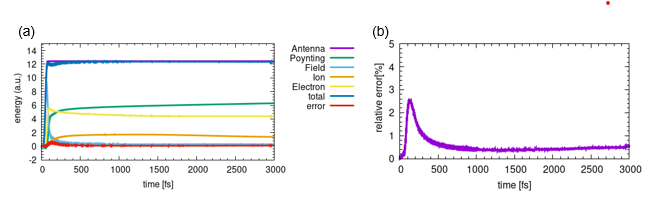
\includegraphics[scale=0.8]{./image/4-7-2rod_dynamics.png}
      \label{fig:4-6}
      \caption{シミュレーション範囲内のエネルギーに関する時間発展図。(a)はアンテナからシステムに入ったエネルギー(Antenna)を紫色、システムから外部に抜け出たエネルギー(Poynting)を緑色、システム内の電磁エネルギー(Field : 電場のエネルギー$\epsilon_0E^{2}/2 +$磁場のエネルギー$B^{2}/2\mu_0$)を水色、イオンによるエネルギー(Ion)を橙色、電子によるエネルギー(Electron)を黄色、合計のエネルギー(total)を赤色で表している。(b)は合計のエネルギー(total)とシステムから外部に抜け出たエネルギー(poynting)の差である相対誤差を表している。}
    \end{center}
  \end{figure}
  
  Antenna(紫色)は、レーザーのエネルギーであり、全体のエネルギー(total、青色)は、場のエネルギー(Field、水色)、電子(Electron、黄色)、イオン(Ion、橙色)のエネルギーを足し合わせた値である。また、poynting は系から抜けだしていくエネルギー(緑色)を表している。まず、レーザーが照射された後、80fs付近から質量の軽い電子はレーザーからエネルギーを得て加速し、その後質量の大きいイオンにエネルギーが移るため、イオンの値が大きくなる。120fs 付近で照射したレーザーがターゲットに反射され系を通り抜け始めるので、poynting の値が大きくなる。また、今回の系では電磁場のエネルギーが完全に減衰することはなく、一定の
  値で下げ止まりになっており、1000 fsまでシステム内に電磁場が保持 (閉じ込め) されていることが分かる。これについては後に詳細に議論する。

  \subsubsection{準定常磁場生成}

  ターゲットにレーザーを照射したときの様子を表すために z 方向の磁場 Bz を示す。
  
  \begin{figure}[H]
    \begin{center}
      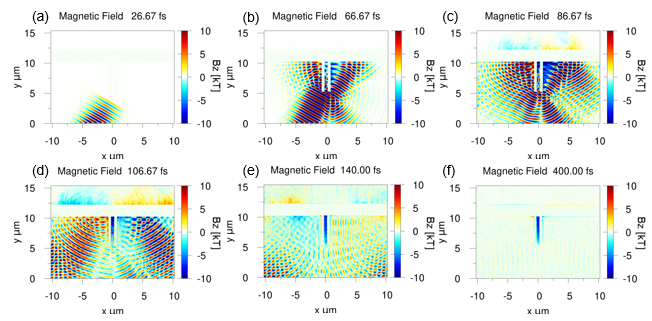
\includegraphics[scale=0.8]{./image/4-13-2rod_Bz.png}
      \label{fig:4-2-3}
      \caption{シミュレーション範囲内のz方向の磁場Bzの図。シミュレーション開始時刻をt=0としている。(a)-(f)はそれぞれ時刻t=26.67fs, 66.67fs, 86.67fs, 106.67fs, 140.00fs, 400.00fsの場合を表している。カラーマップはz方向の磁場Bzを-10~10kTで表している。}
    \end{center}
  \end{figure}
  図4.3はレーザーが照射されている様子を表している。(a),はレーザーが図の左下からレーザーが照射されているフェーズである。(b),(c),(d)はレーザーがターゲットに当たり2本のロッドの間に侵入しているフェーズであり、その際に電子がレーザー照射方向にポンデロモーティブ力によって加速されることによって磁場が形成されている。(e),(f)はレーザーがターゲットに反射されてた後の磁場の様子を表している。(f)からもわかるようにレーザーが照射されてからターゲットに反射してしばらくたった時間では、強い準定常磁場が2本のロッドの間に生成されていることがわかる。このように構造性媒質としてµmオーダーの2本のロッドを導入すると、単純な媒質のスラブターゲットの場合の\ref*{fig:4-4}とは異なりkTオーダの準定常な強磁場が生成される。

  \subsubsection{電磁場エネルギーの時間発展}
  2本のロッドターゲットにレーザーが照射された際のシュミレーション範囲内の電磁場エネルギーの時間発展を示す。
  
  \begin{figure}[H]
    \begin{center}
      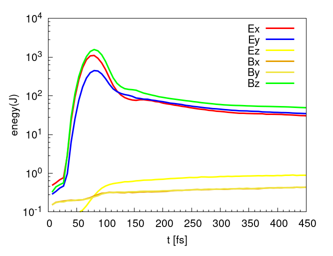
\includegraphics[scale=1]{./image/4-15-2rod.png}
      \label{fig:4-4-4}
      \caption{シュミレーション範囲内の電磁場エネルギーの時間発展}
    \end{center}
  \end{figure}
  
  シュミレーション範囲内の電磁場エネルギーの時間発展の図。赤色はEx,青色はEy,緑色はBzのエネルギーを表している。
  スラブターゲットの時と比べ磁場エネルギーが保存している。


  \subsubsection{反磁性電流}
  上記で、µmオーダーのロッドを導入することで準定常な磁場ができることがわかった。ここでは磁場が保持されるメカニズムについて述べる。
  磁場を保持するメカニズムを探るため、電流源を確認する。磁場配位は図\ref{fig:4-2-5}に示すとおり特徴的な配位であり、マクスウェル方程式から、これを積極的に保持する電流の駆動が示唆される。磁場が保持されている t=400 fs における電流 Jy は以下のとおりである。
  
  \begin{figure}[H]
    \begin{center}
      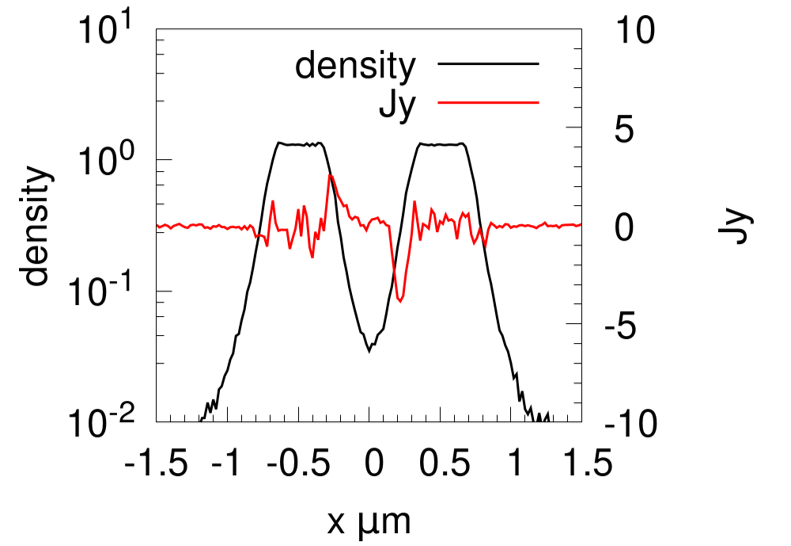
\includegraphics[scale=0.5]{./image/4-14-2rod.png}
      \label{fig:4-2-5}
      \caption{電流Jyをロッド方向に平均したもの。}
    \end{center}
  \end{figure}
  
  y 方向に流れる電流は、ロッドの表面付近で左右対象に駆動していることが確認できる。一方で、レーザーとの相互作用を経てロッド表面には電子の圧力勾配が生まれる。$\\$
  
  ここまでを模式的に示したものが図\ref{fig:4-2-6}である。
  \begin{figure}[H]
    \begin{center}
      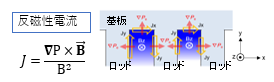
\includegraphics[scale=1.7]{./image/4-16-2rod.png}
      \label{fig:4-2-6}
      \caption{電流}
    \end{center}
  \end{figure}
  
  このとき $\textit{\textbf{B}} \times \nabla \textit{\textbf{P}}_e$ による電流が駆動され、この直線電流により磁場が保持されている。
  実際にシミュレーションをした磁場と電流の様子を図\ref{fig:4-2-7}に示す。
  
  \begin{figure}[H]
    \begin{center}
      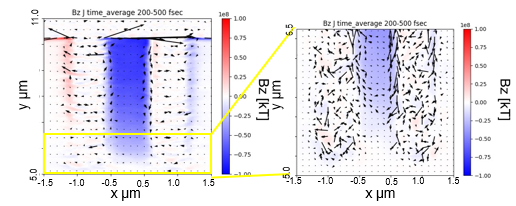
\includegraphics[scale=1]{./image/4-17-2rod.png}
      \label{fig:4-2-7}
      \caption{磁場Bzと電流。(a)は2本のロッドとその間の範囲の磁場Bzと電流の矢印の図。(b)は(a)の黄色の線の範囲を拡大し電流の矢印を大きくした図。}
    \end{center}
  \end{figure}
  
  図\ref{fig:4-2-7}より、(a)ロッドの表面上(粒子の圧力勾配が大きい場所)に電流が強く流れている。ロッドの先端部分に流れる電流は、ロッドの付け根に流れる電流より小さくのは粒子の圧力勾配の差があるからだと考えられる。
  図\ref{fig:4-2-7}からもわかるように、$\textit{\textbf{B}} \times \nabla \textit{\textbf{P}}_e$ による反磁性電流 $\textit{\textbf{v}}_D$ よって磁場が保持されている。


  \subsubsection{レーザー照射の角度依存性}
  ここでレーザーの照射角度$ \theta $を変えた時の磁場の様子を調べる。
  
  \begin{figure}[H]
    \begin{center}
      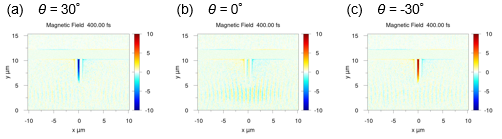
\includegraphics[scale=1]{./image/4-19-2rod.png}
      \label{fig:4-4-3}
      \caption{シミュレーション範囲内のレーザー照射角度$\theta$=30, 0, -30それぞれの磁場。(a)は$\theta$=30、(b)$\theta$=0、(c)$\theta$=-30}
    \end{center}
  \end{figure}
  
  $\theta$=30, -30は、系内に滞留する磁場はロッド間に保持されていることは同じだが、磁場の向きは逆である。$\theta$=0は強い準定常磁場はできていない。このように磁場配位はレーザーの入射角度に依存していることが分かった。

\subsection{マルチロッドターゲットへのシミュレーション}
ここでは、ロッドの本数を2本から10本に増やした系を示す。

\subsubsection{シミュレーション条件}
シミュレーションは図 に示す通り、x 方向のシステムサイズ Lx = 20.48μm、y 方向のシステムサイズ Ly = 15.36μm の長方形の領域を設定し、y 方向の 10~12μm の範囲にスラブターゲットと10本のロッド径が0.5μmのロッドを配置した。

\begin{figure}[H]
  \begin{center}
    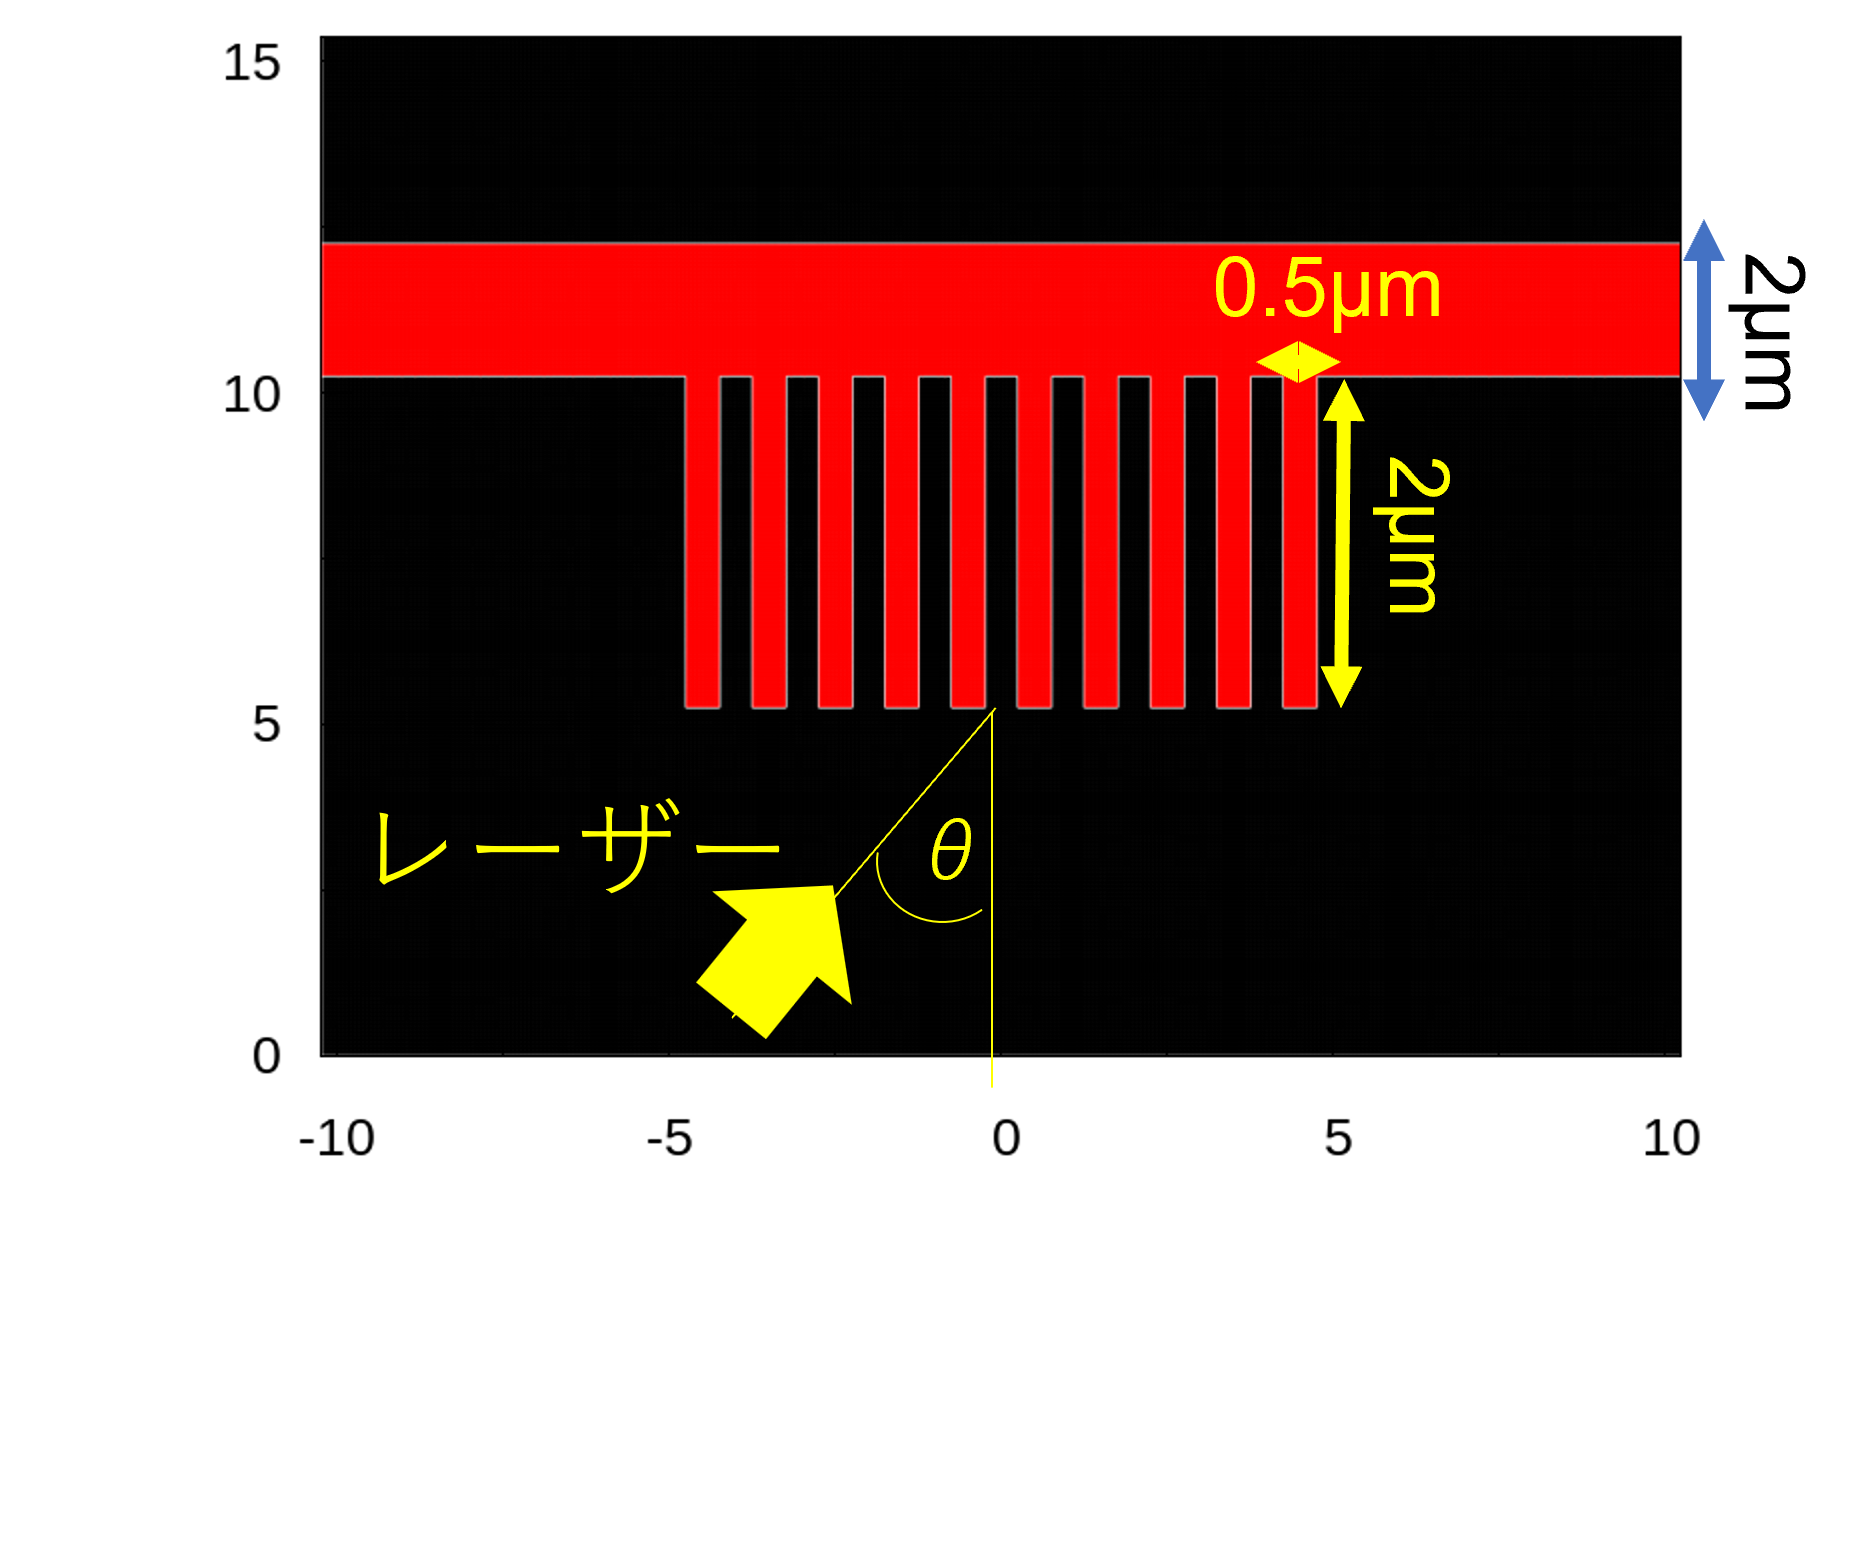
\includegraphics[scale=0.4]{./image/4-9-10rod.png}
    \label{fig:4-8}
    \caption{スラブターゲットと10本ロッドの図}
  \end{center}
\end{figure}

この系に対して、スラブターゲットに照射したレーザーと同様のパルス幅が 40 fs(FWHM)、最大集光強度が$1.2×10^{19}W/cm^2$に達する高強度レーザーを +y方向から$\theta=$30度の角度で照射した。ここで、レーザーは y=40 nm に設置したアンテナから誘導電流を流すことにより発振させており、粒子 (電子とイオン)・場 (電場・磁場) ともに、xy 方向に透過(吸収)境界条件を課している。詳細なシミュレーション条件は表に示す。

\begin{table}[H]
  \begin{center}
    \caption{シミュレーション設定}
  \begin{tabular}{|l|r|} \hline
    \multicolumn{2}{|c|}{レーザー条件} \\ \hline
    レーザー強度 & $\textit{I}=1.2\times  10^{19}[W/cm^2]$ \\ 
    規格化強度 & $\textit{a} _0 = 2.39$ \\
    パルス幅 & 40fsec \\ 
    レーザープロファイル(波形)[時間方向] & ガウシアン \\
    レーザー空間分布 & 平面波 \\
    カットオフ密度 & $\textit{n} _c = 1.7 \time 10^21 [cm^{-3}]$ \\\hline
    \multicolumn{2}{|c|}{ターゲット条件} \\ \hline
    イオンの種類 & ケイ素(Si) \\
    電子密度 &$6.98 \times  10 ^{23} [\rm{cm}^{-3}]$ \\
    ロッド直径 & 0.5[$\mu$ m] \\
    ロッドの長さ & 10[$\mu$ m]  \\ \hline
    \multicolumn{2}{|c|}{系} \\ \hline
    システムサイズ(x方向) & [20.48$\mu $m] \\
    システムサイズ(y方向) & [15.36$\mu $m] \\
    メッシュ数(x方向) & [1024] \\
    メッシュ数(y方向) & [768] \\
    メッシュ幅(x方向) & [20nm] \\
    メッシュ幅(y方向) & [20nm] \\
    時間幅 & $1/6$[fs] \\ \hline
    \multicolumn{2}{|c|}{境界条件} \\ \hline
    粒子(x方向) & 周期 \\
    粒子(y方向) & 透過 \\
    電磁波(x方向) & 周期 \\
    電磁波(y方向) & 透過 \\ \hline
  \end{tabular}
  \end{center}
  \end{table}

  \subsubsection{エネルギーダイナミクス}
  はじめに、系のエネルギーダイナミクスを示す。横軸は時間、縦軸は規格化したエネルギーを表している。
  
  \begin{figure}[H]
    \begin{center}
      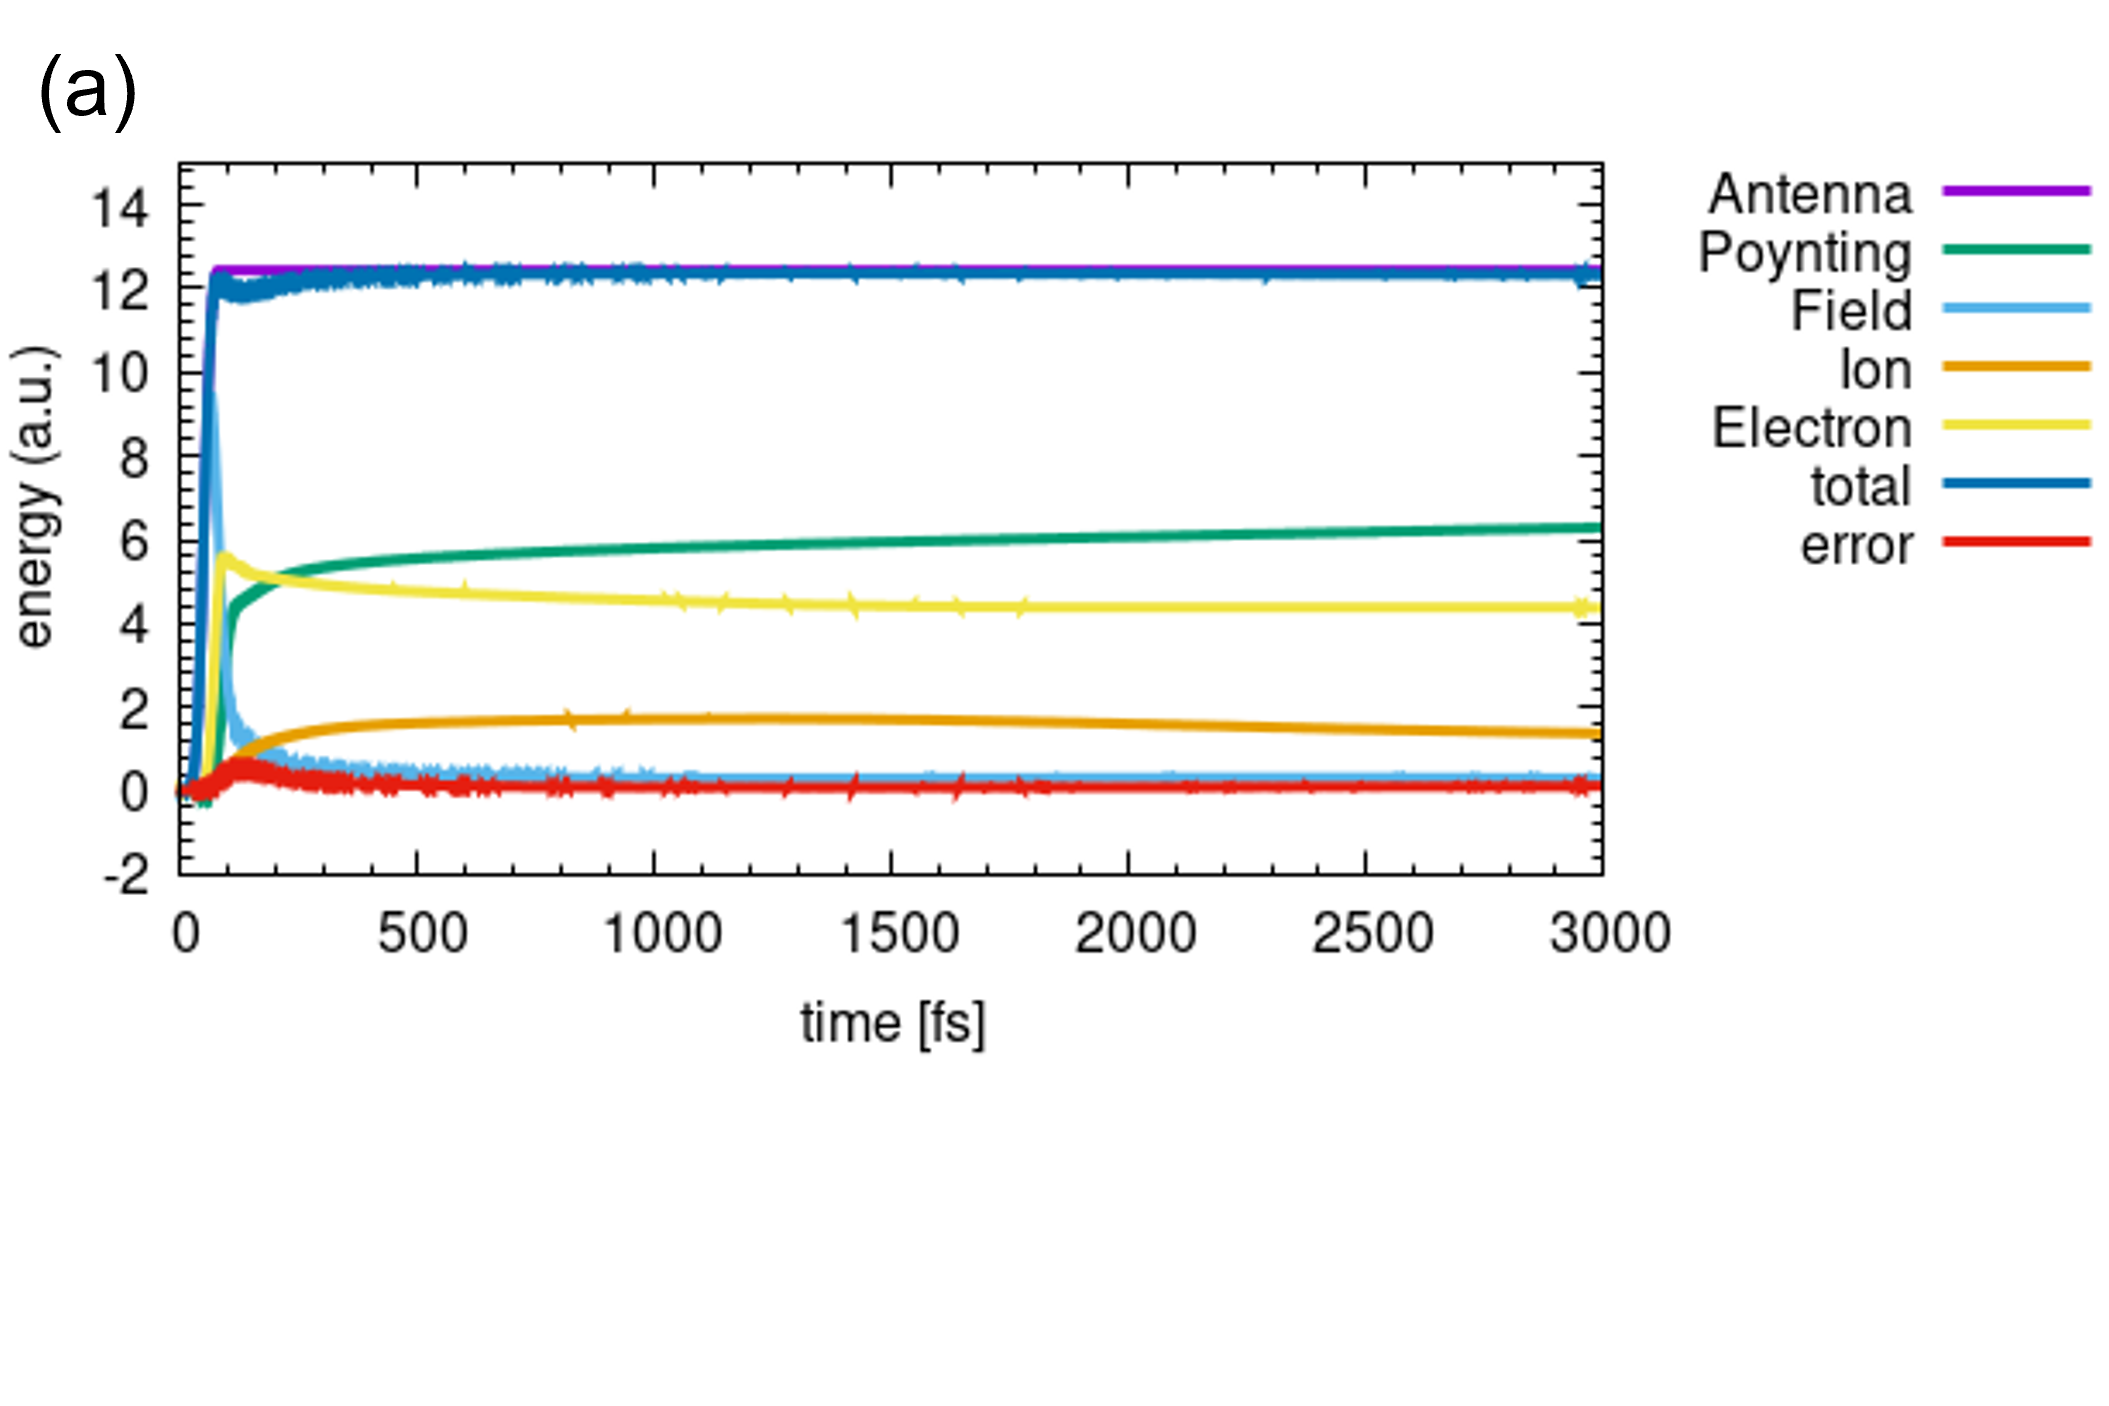
\includegraphics[scale=0.5]{./image/4-10-10rod_dynamics.png}
      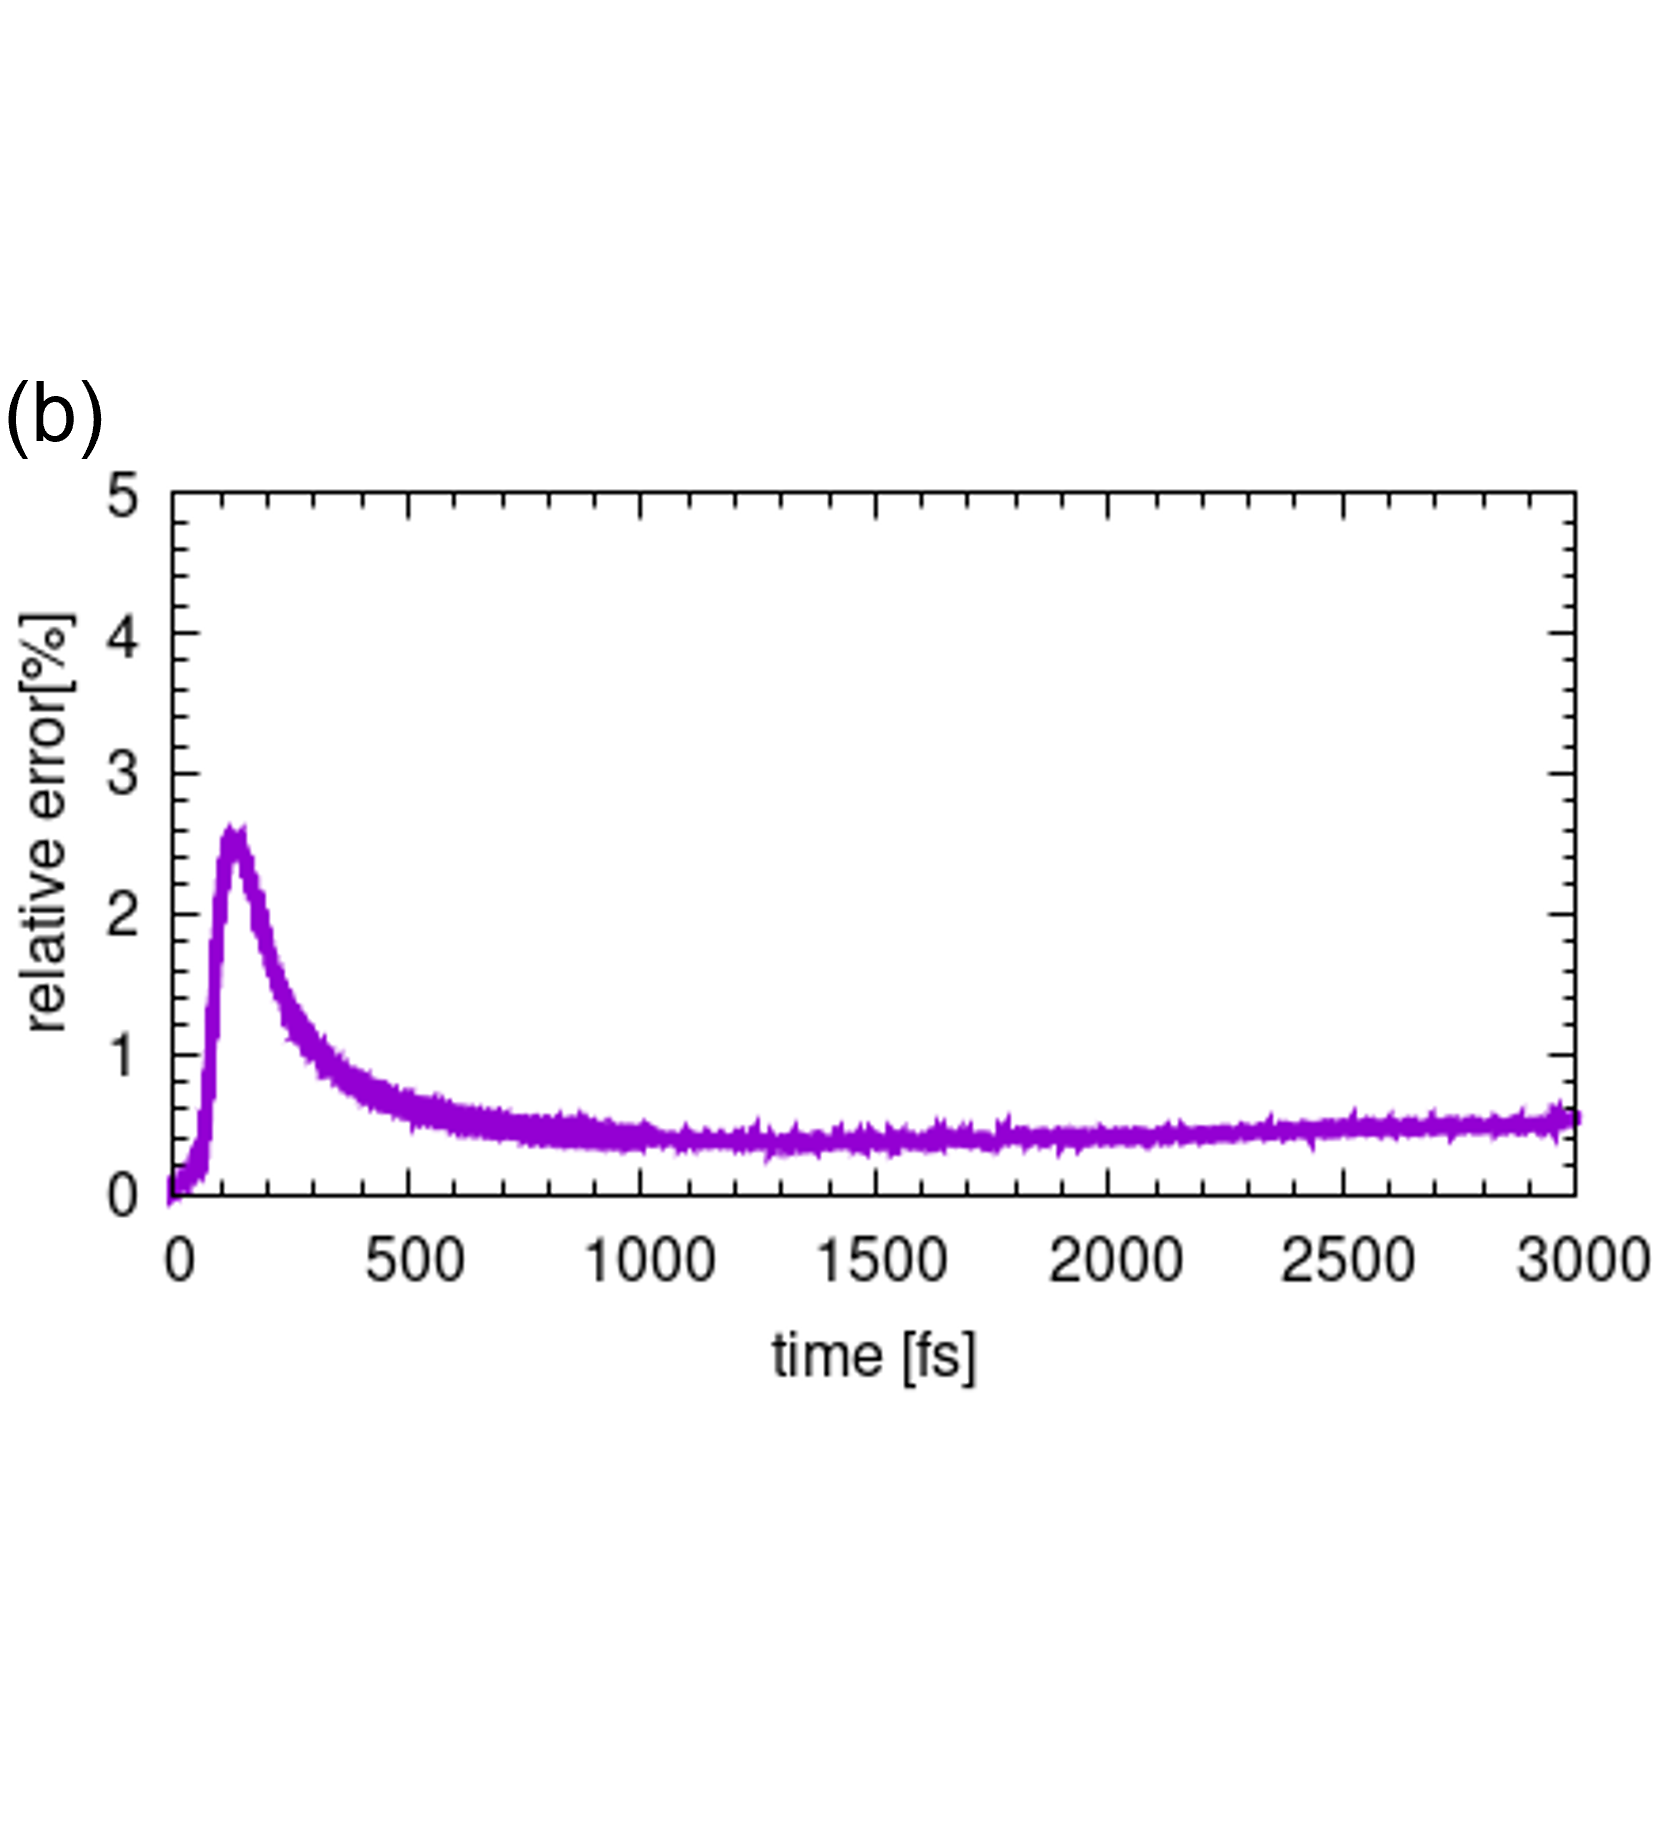
\includegraphics[scale=0.5]{./image/4-11-10rod_dynamics_error.png}
      \label{fig:4-7}
      \caption{シミュレーション範囲内のエネルギーに関する時間発展図。(a)はアンテナからシステムに入ったエネルギー(Antenna)を紫色、システムから外部に抜け出たエネルギー(Poynting)を緑色、システム内の電磁エネルギー(Field : 電場のエネルギー$\epsilon_0E^{2}/2 +$磁場のエネルギー$B^{2}/2\mu_0$)を水色、イオンによるエネルギー(Ion)を橙色、電子によるエネルギー(Electron)を黄色、合計のエネルギー(total)を赤色で表している。(b)は合計のエネルギー(total)とシステムから外部に抜け出たエネルギー(poynting)の差である相対誤差を表している。}
    \end{center}
  \end{figure}
  
  Antenna(紫色)は、レーザーのエネルギーであり、全体のエネルギー(total、青色)は、場のエネルギー(Field、水色)、電子(Electron、黄色)、イオン(Ion、橙色)のエネルギーを足し合わせた値である。また、poynting は系から抜けだしていくエネルギー(緑色)を表している。まず、レーザーが照射された後、80fs付近から質量の軽い電子はレーザーからエネルギーを得て加速し、その後質量の大きいイオンにエネルギーが移るため、イオンの値が大きくなる。120fs 付近で照射したレーザーがターゲットに反射され系を通り抜け始めるので、poynting の値が大きくなる。また、今回の系では電磁場のエネルギーが完全に減衰することはなく、一定の
  値で下げ止まりになっており、3000 fsまでシステム内に電磁場が保持 (閉じ込め) されていることが分かる。これについては後に詳細に議論する。

  \subsubsection{準定常磁場生成}

  ターゲットにレーザーを照射したときの様子を表すために z 方向の磁場 Bz を示す。
  
  \begin{figure}[H]
    \begin{center}
      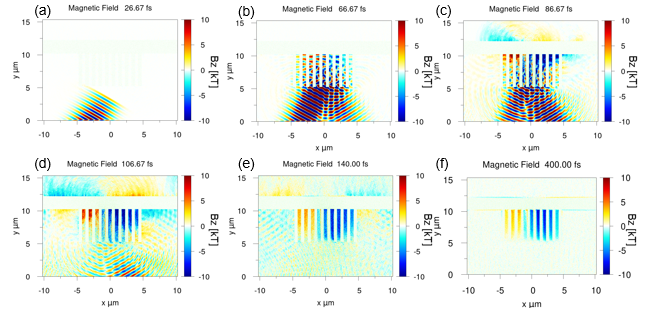
\includegraphics[scale=0.8]{./image/4-20-10rod.png}
      \label{fig:4-9}
      \caption{シミュレーション範囲内のz方向の磁場Bzの図。シミュレーション開始時刻をt=0としている。(a)-(f)はそれぞれ時刻t=26.67fs, 66.67fs, 86.67fs, 106.67fs, 140.00fs, 400.00fsの場合を表している。カラーマップはz方向の磁場Bzを-10~10kTで表している。}
    \end{center}
  \end{figure}
  図4.3はレーザーが照射されている様子を表している。(a),はレーザーが図の左下からレーザーが照射されているフェーズである。(b),(c)はレーザーがターゲットに当たり10本のロッドの間に侵入しているフェーズであり、その際に電子がレーザー照射方向にポンデロモーティブ力によって加速されることによって磁場が形成されている。(d),(e),(f)はレーザーがターゲットに反射されてた後の磁場の様子を表している。(f)からもわかるようにレーザーが照射されてからターゲットに反射してしばらくたった時間では、強い準定常磁場がロッドの間に生成されていることがわかる。このように構造性媒質としてµmオーダーの2本のロッドを導入すると、単純な媒質のスラブターゲットの場合の\ref*{fig:4-4}とは異なりkTオーダの準定常な強磁場が生成される。
  
  \subsection{ロッドの直径依存性}
  レーザーを構造性媒質に照射する際のプラズマ制御に向けた、より良いパラメータを探す目的で同一の空間充填率でロッド径を0.125μm, 0.25μm, 0.5μm, 1.0μmで変化させた場合に生成する磁場強度の時間変化を詳細に調べた。
  
  \subsubsection{シミュレーション条件}
  シミュレーションは図 に示す通り、x 方向のシステムサイズ Lx = 20.48μm、y 方向のシステムサイズ Ly = 15.36μm の長方形の領域を設定し、y 方向の 10~12μm の範囲にスラブターゲットと10本のロッド径がそれぞれ(a)1μm, (b)0.5μm, (c)0.25μm, (d)0.125μmのロッドを配置した。
  
  \begin{figure}[H]
    \begin{center}
      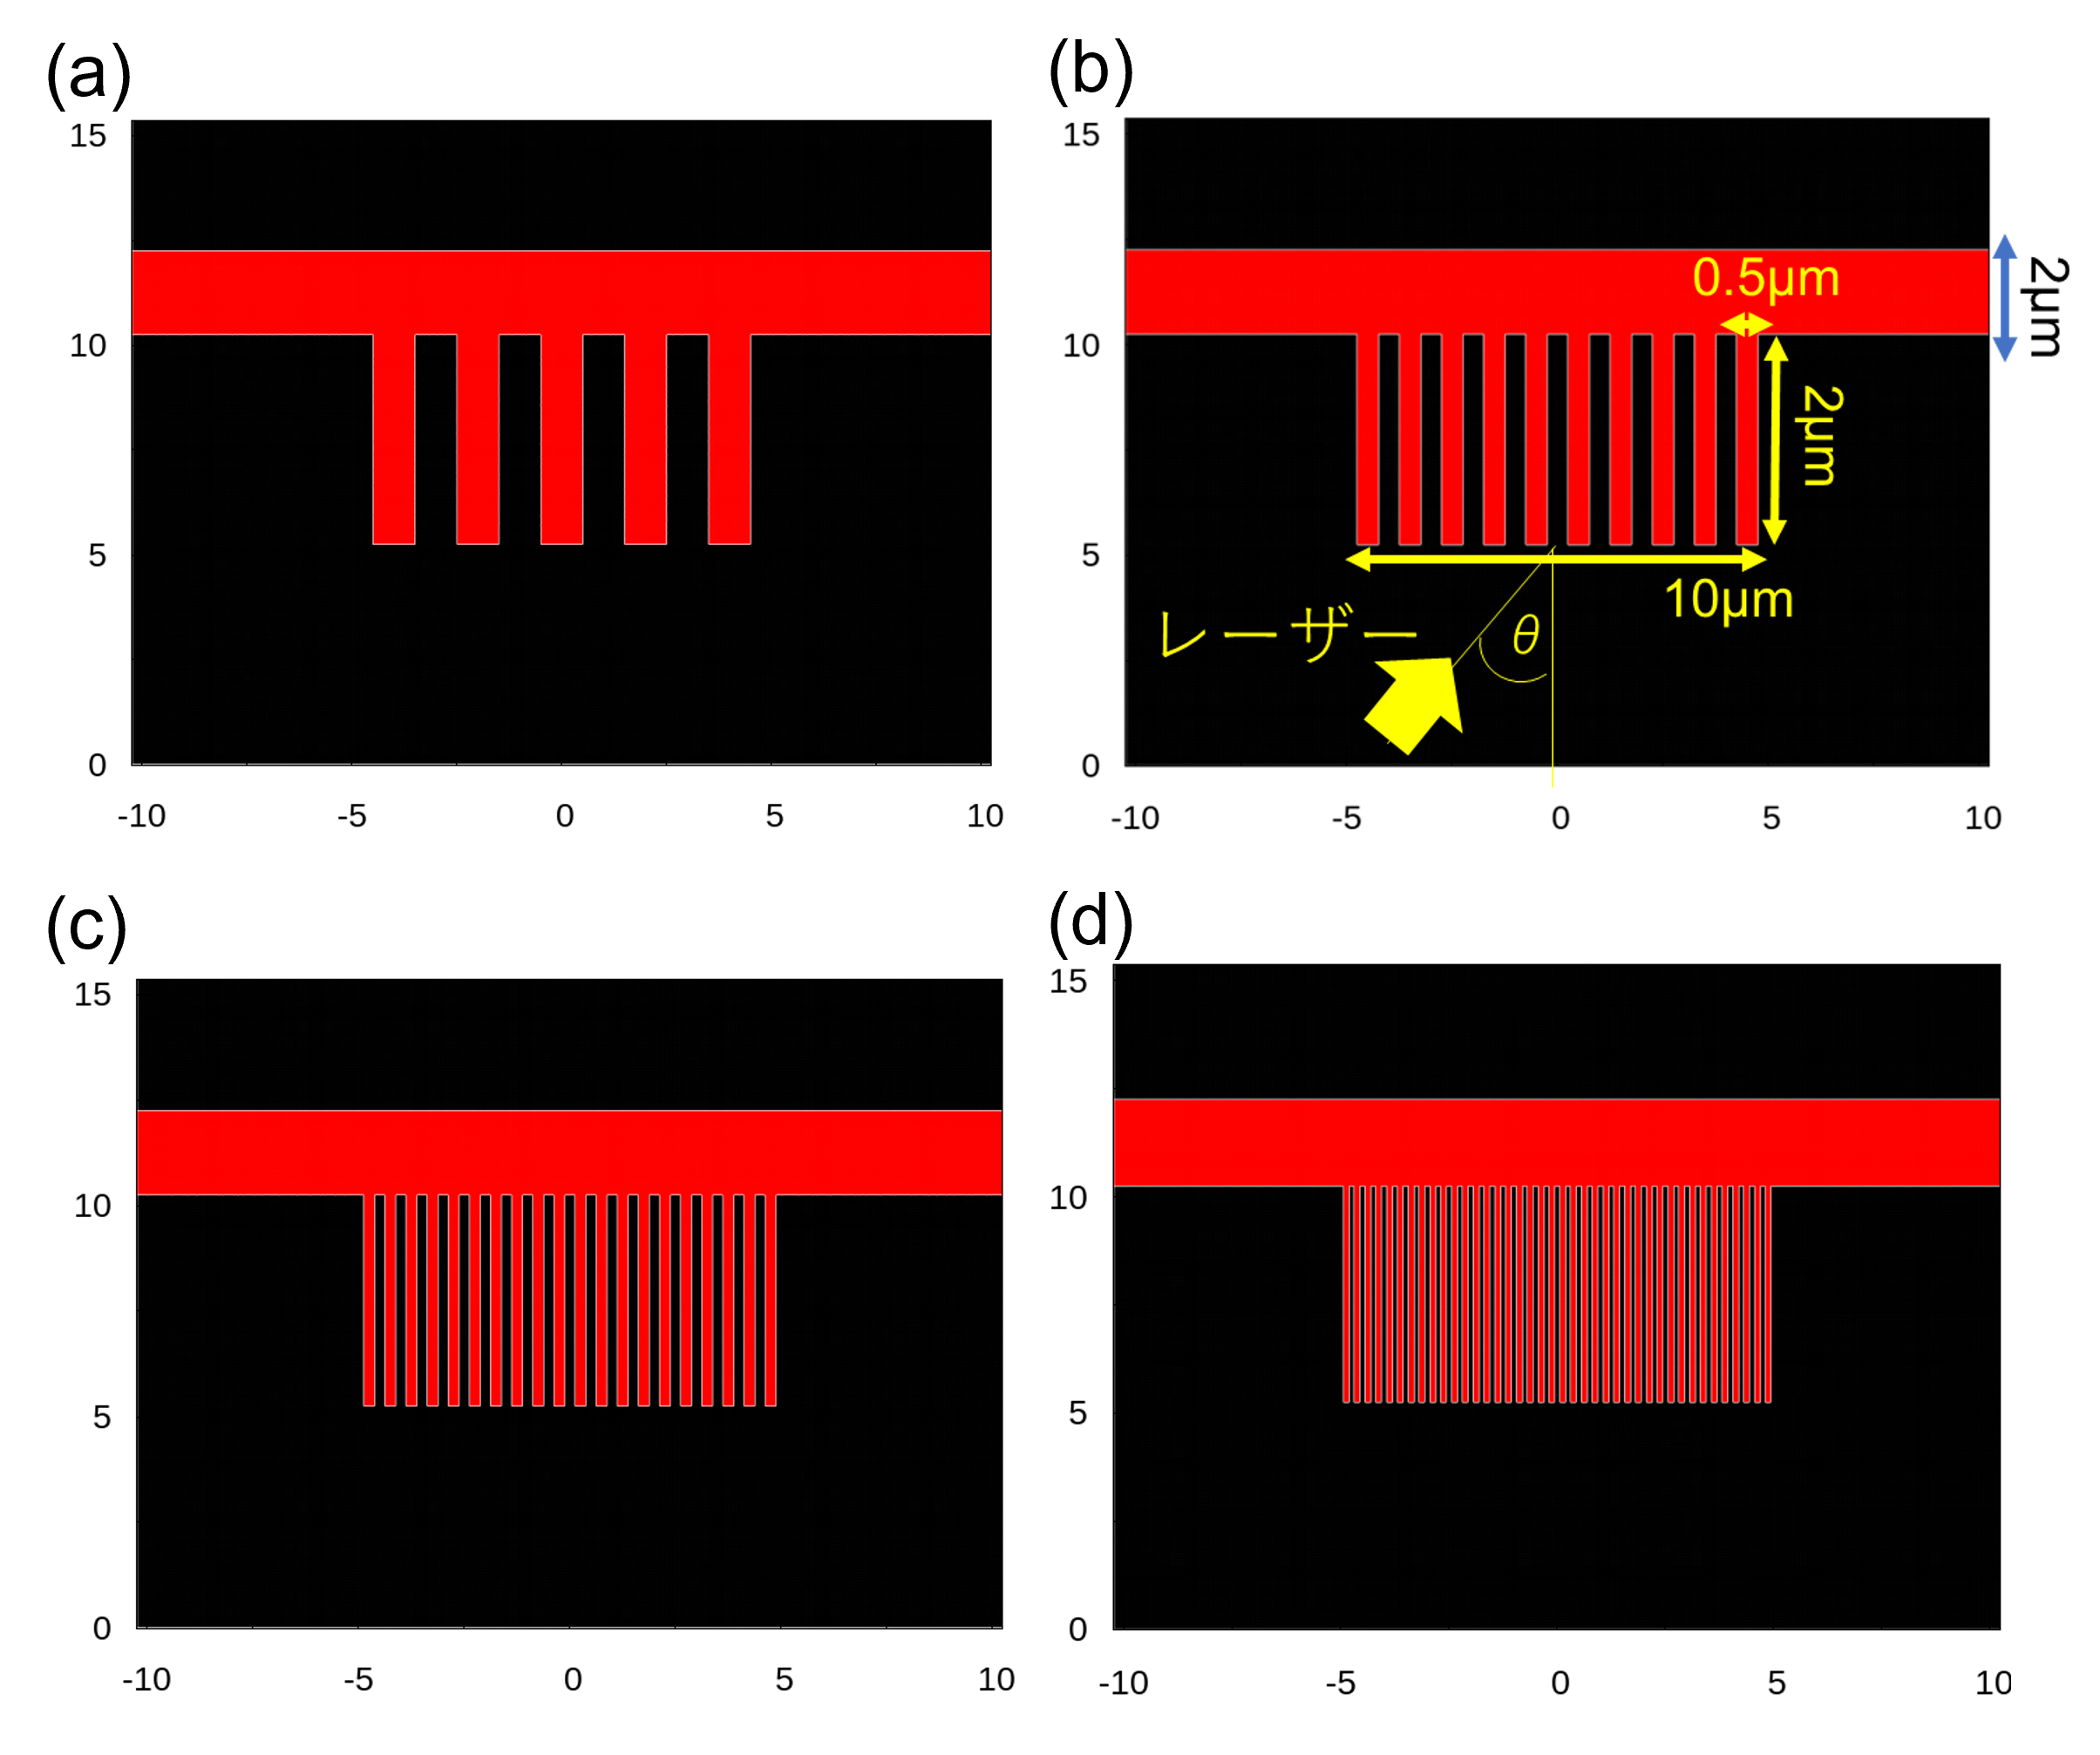
\includegraphics[scale=0.6]{./image/4-12-10rod_4.png}
      \label{fig:4-8-2}
      \caption{スラブターゲットと10本ロッドのロッド径が異なる4パターンの図}
    \end{center}
  \end{figure}
  
  この系に対して、スラブターゲットに照射したレーザーと同様のパルス幅が 40 fs(FWHM)、最大集光強度が$1.2×10^{19}W/cm^2$に達する高強度レーザーを +y方向から$\theta=$30度の角度で照射した。ここで、レーザーは y=40 nm に設置したアンテナから誘導電流を流すことにより発振させており、粒子 (電子とイオン)・場 (電場・磁場) ともに、xy 方向に透過(吸収)境界条件を課している。詳細なシミュレーション条件は表に示す。
  
  \begin{table}[H]
    \begin{center}
      \caption{シミュレーション設定}
    \begin{tabular}{|l|r|} \hline
      \multicolumn{2}{|c|}{レーザー条件} \\ \hline
      レーザー強度 & $\textit{I}=1.2\times  10^{19}[W/cm^2]$ \\ 
      規格化強度 & $\textit{a} _0 = 2.39$ \\
      パルス幅 & 40fsec \\ 
      レーザープロファイル(波形)[時間方向] & ガウシアン \\
      レーザー空間分布 & 平面波 \\
      カットオフ密度 & $\textit{n} _c = 1.7 \time 10^21 [cm^{-3}]$ \\\hline
      \multicolumn{2}{|c|}{ターゲット条件} \\ \hline
      イオンの種類 & ケイ素(Si) \\
      電子密度 &$6.98 \times  10 ^{23} [\rm{cm}^{-3}]$ \\
      ロッド直径 & (a)1, (b)0.5, (c)0.25, (d)0.125[$\mu$ m] \\
      ロッドの長さ & 10[$\mu$ m]  \\ \hline
      \multicolumn{2}{|c|}{系} \\ \hline
      システムサイズ(x方向) & [20.48$\mu $m] \\
      システムサイズ(y方向) & [15.36$\mu $m] \\
      メッシュ数(x方向) & [1024] \\
      メッシュ数(y方向) & [768] \\
      メッシュ幅(x方向) & [20nm] \\
      メッシュ幅(y方向) & [20nm] \\
      時間幅 & $1/6$[fs] \\ \hline
      \multicolumn{2}{|c|}{境界条件} \\ \hline
      粒子(x方向) & 周期 \\
      粒子(y方向) & 透過 \\
      電磁波(x方向) & 周期 \\
      電磁波(y方向) & 透過 \\ \hline
    \end{tabular}
    \end{center}
    \end{table}

    \subsubsection{準定常磁場生成}

    ロッド径を変えた時の磁場の様子を示す。
    
    \begin{figure}[H]
      \begin{center}
        \includegraphics[scale=0.5]{./image/4-21-10rod.png}
        \label{fig:4-10}
        \caption{シミュレーション範囲内のz方向の磁場Bzの図。シミュレーション開始時刻をt=0としている。(a)ロッド径1µm, (b)ロッド径0.5µm, (c)ロッド径0.25µm, (d)ロッド径0.125µmのそれぞれ400fsの様子を表している。}
      \end{center}
    \end{figure}
    図\ref*{fig:4-10}からわかるように、ロッド径を変えてもkTオーダの準定常な強磁場が生成される。

    \subsubsection{磁場エネルギーの保存}
    ロッド径の違いによる磁場エネルギーの保存の違いについて示す。
    
    
    \begin{figure}[H]
      \begin{center}
        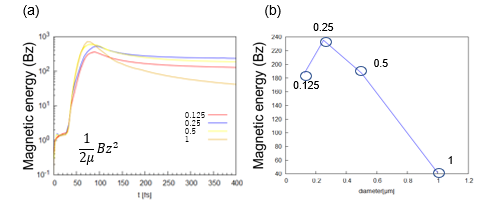
\includegraphics[scale=1]{./image/4-22-10rod.png}
        \label{fig:4-11}
        \caption{磁場エネルギー(Bz)の時間発展。(a)の赤色は0.125µm, 青色は0.25µm, 黄色は0.5µm, 橙黄色は1µmのロッド径の磁場エネルギー(Bz)の時間発展である。(b)の縦軸は(a)の400fsの磁場エネルギー、横軸はロッド径である。}
      \end{center}
    \end{figure}
    
    ロッド径が0.25µmの時に磁場エネルギーを一番保持することを示している。

    \subsubsection{エネルギーの吸収特性}

    これまでの結果より、構造性媒質に高強度レーザーを照射すると、レーザーから媒質の各粒子のエネルギーや電磁場エネルギーへとエネルギーのが移り変わり、準定常磁場が生成されることが明らかになった。ここでは、レーザーのエネルギーが構造性媒質のどの部分で吸収されるのかを調べる。具体的にはロッドターゲットの各所でのポインティングフラックス$S=E \times B $を評価し(図\ref{fig:4-26}参照)、その面での通過する電磁波のエネルギーの値を求めることでロッドターゲットのエネルギーの吸収特性を調べることができる。 $\\$
    
    \begin{figure}[H]
      \begin{center}
        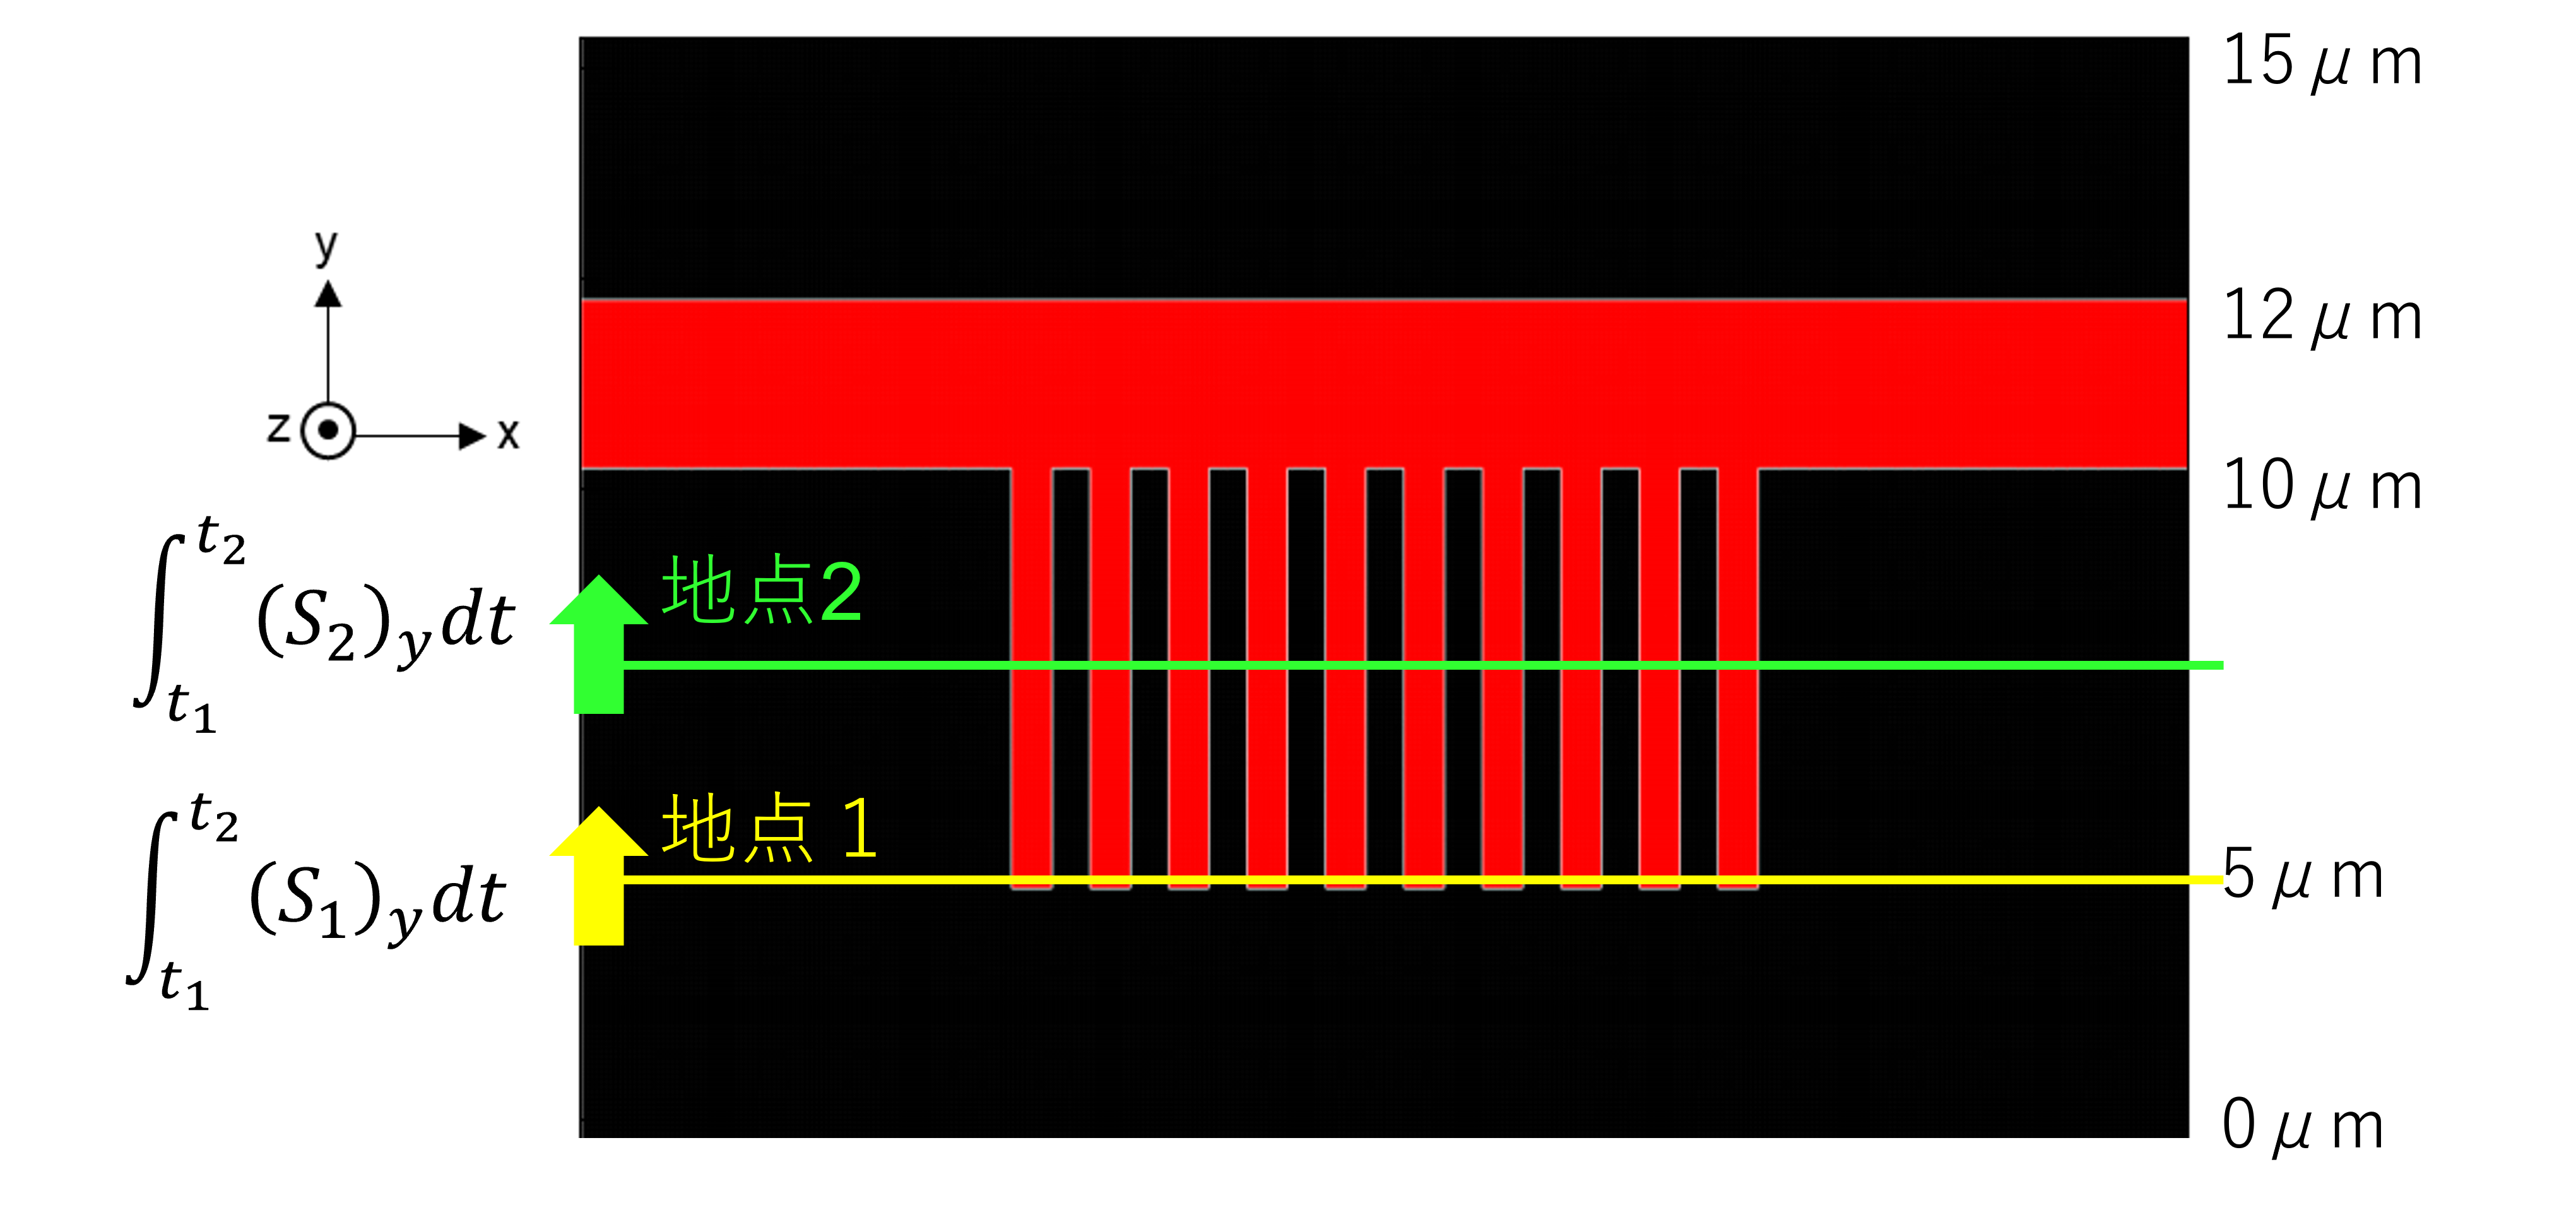
\includegraphics[scale=0.4]{./image/4-26.png}
        \label{fig:4-26}
        \caption{ロッドターゲットの系。y方向の各地点でポインティングフラックスを計算しロッドの高さ方向(y方向)に関する吸収率及び伝搬過程を調べる。例えば地点1と地点2のポインティングフラックスが同じであれば、電磁波のエネルギーは地点1から地点2の間では吸収されておらず100%透過していることを示す。一方、地点1と地点2のポインティングフラックスに差があれば、電磁波のエネルギーは地点1から地点2の間でその差の分吸収されていることを表す。}
      \end{center}
    \end{figure}
    
    
    \begin{figure}[H]
      \begin{center}
        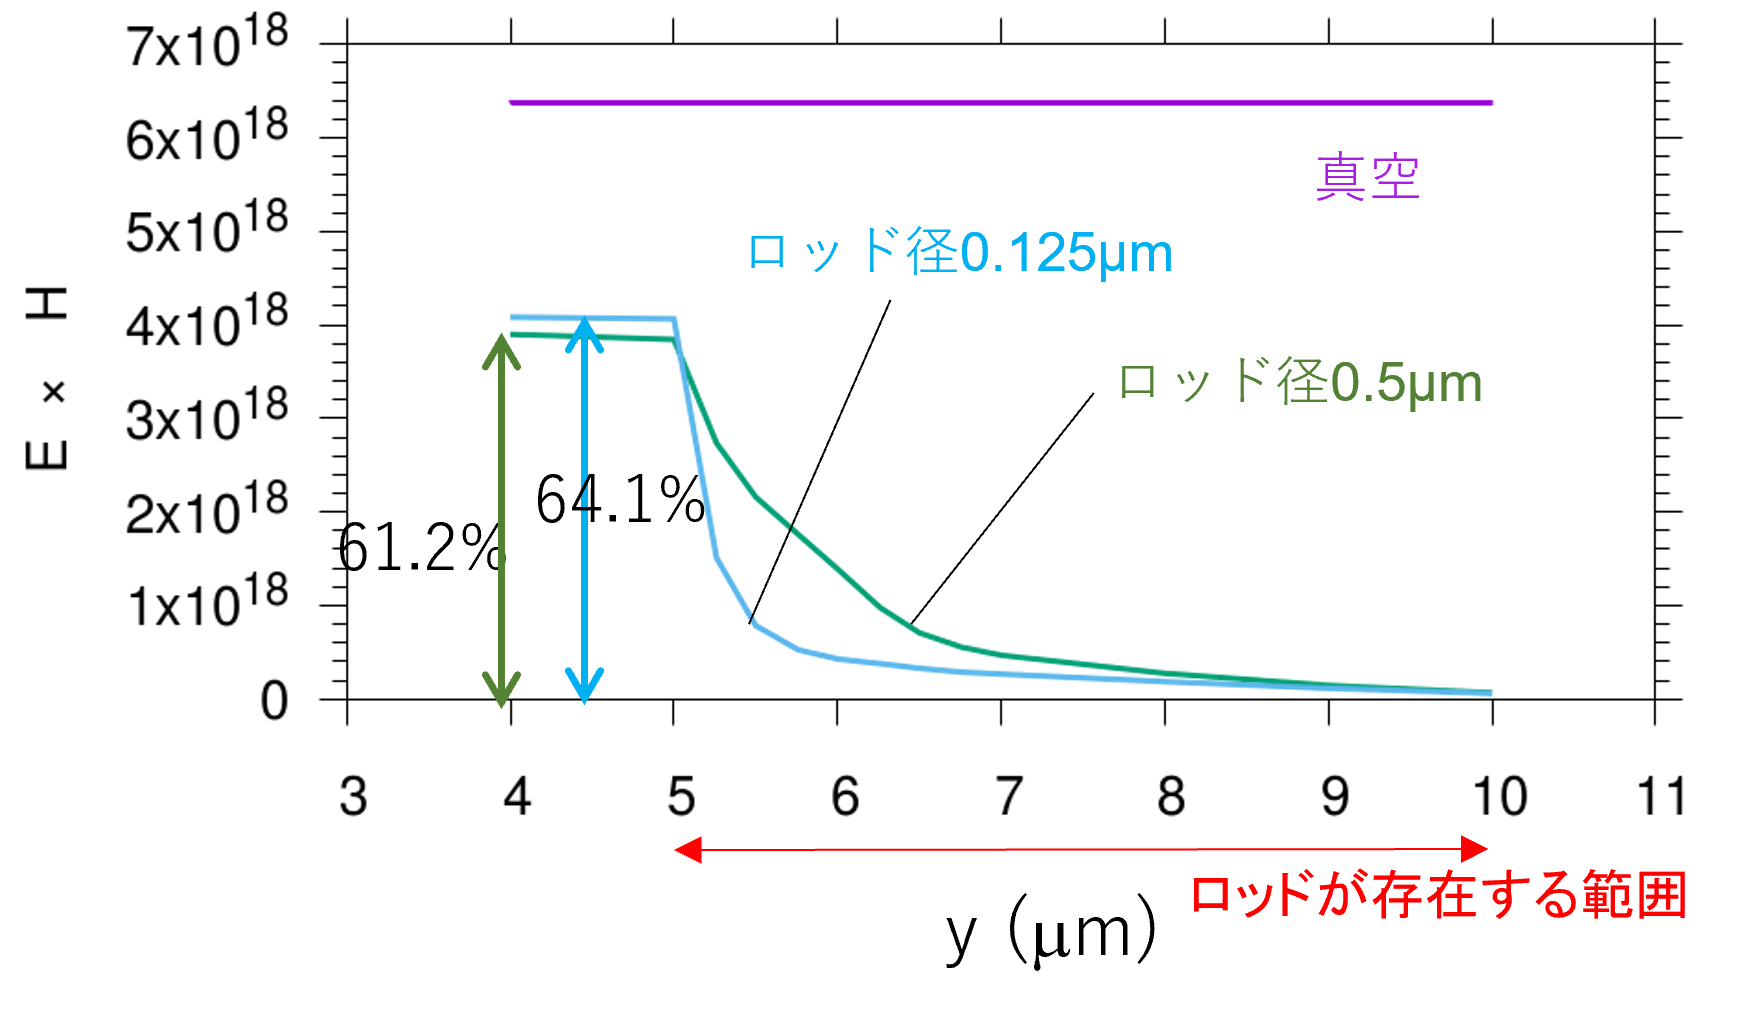
\includegraphics[scale=1]{./image/4-27.png}
        \label{fig:4-27}
        \caption{ロッドターゲットのy方向の各点におけるポインティングフラックス。縦軸はポインティングフラックス$S=E \times B$、横軸はロッドの高さ方向のy座標を表す。横軸の5-10μmの範囲はロッドターゲットが存在する範囲である。紫色の線は真空にレーザーを照射したときの結果、緑色はロッド径が0.5μm、水色はロッド径が0.125μmの結果を表している。}
      \end{center}
    \end{figure}
    
    真空の場合の場合のポインティングフラックスは、どこにも吸収されることがないので一定の値を保っているが、ロッド径が0.5µmと0.125µmの系は、入力されたレーザーエネルギーの約40%がロッドの前面で反射されるため、真空の場合と比べると約60%ほどのエネルギーがロッド内に入っていっていくことがわかる。この60%というのは、この系、全体での吸収率と対応しているため、妥当な結果だと考えられる。
    
    レーザーがロッドに内に入った後はロッド径が0.5µm, 0.125µmの系いずれも、ロッドの前端付近(y=5-7付近)でレーザーのエネルギーの大部分吸収されることがわかった。またロッド径が0.125µmのポインティングフラックスの減衰率は、0.5µmの減衰率より大きいことを示している。このことからロッド径が短いほどロッドの内部にレーザーが侵入できることが分かった。    

\subsection{レーザー強度依存性}
レーザーを構造性媒質に照射する際のプラズマ制御に向けた、より良いパラメータを探す目的で同一ターゲットに照射するレーザー強度を変化させた場合に生成す$I=1.2\times 10^{18}, 1.2\times 10^{19}, 1.2\times 10^{20}, 1.2\times 10^{21}[W/cm^2]$る磁場強度の時間変化を詳細に調べた。

\subsubsection{シミュレーション条件}
シミュレーションは図 に示す通り、x 方向のシステムサイズ Lx = 20.48μm、y 方向のシステムサイズ Ly = 15.36μm の長方形の領域を設定し、y 方向の 10~12μm の範囲にスラブターゲットと10本のロッド径が0.5μmのロッドを配置した。

\begin{figure}[H]
  \begin{center}
    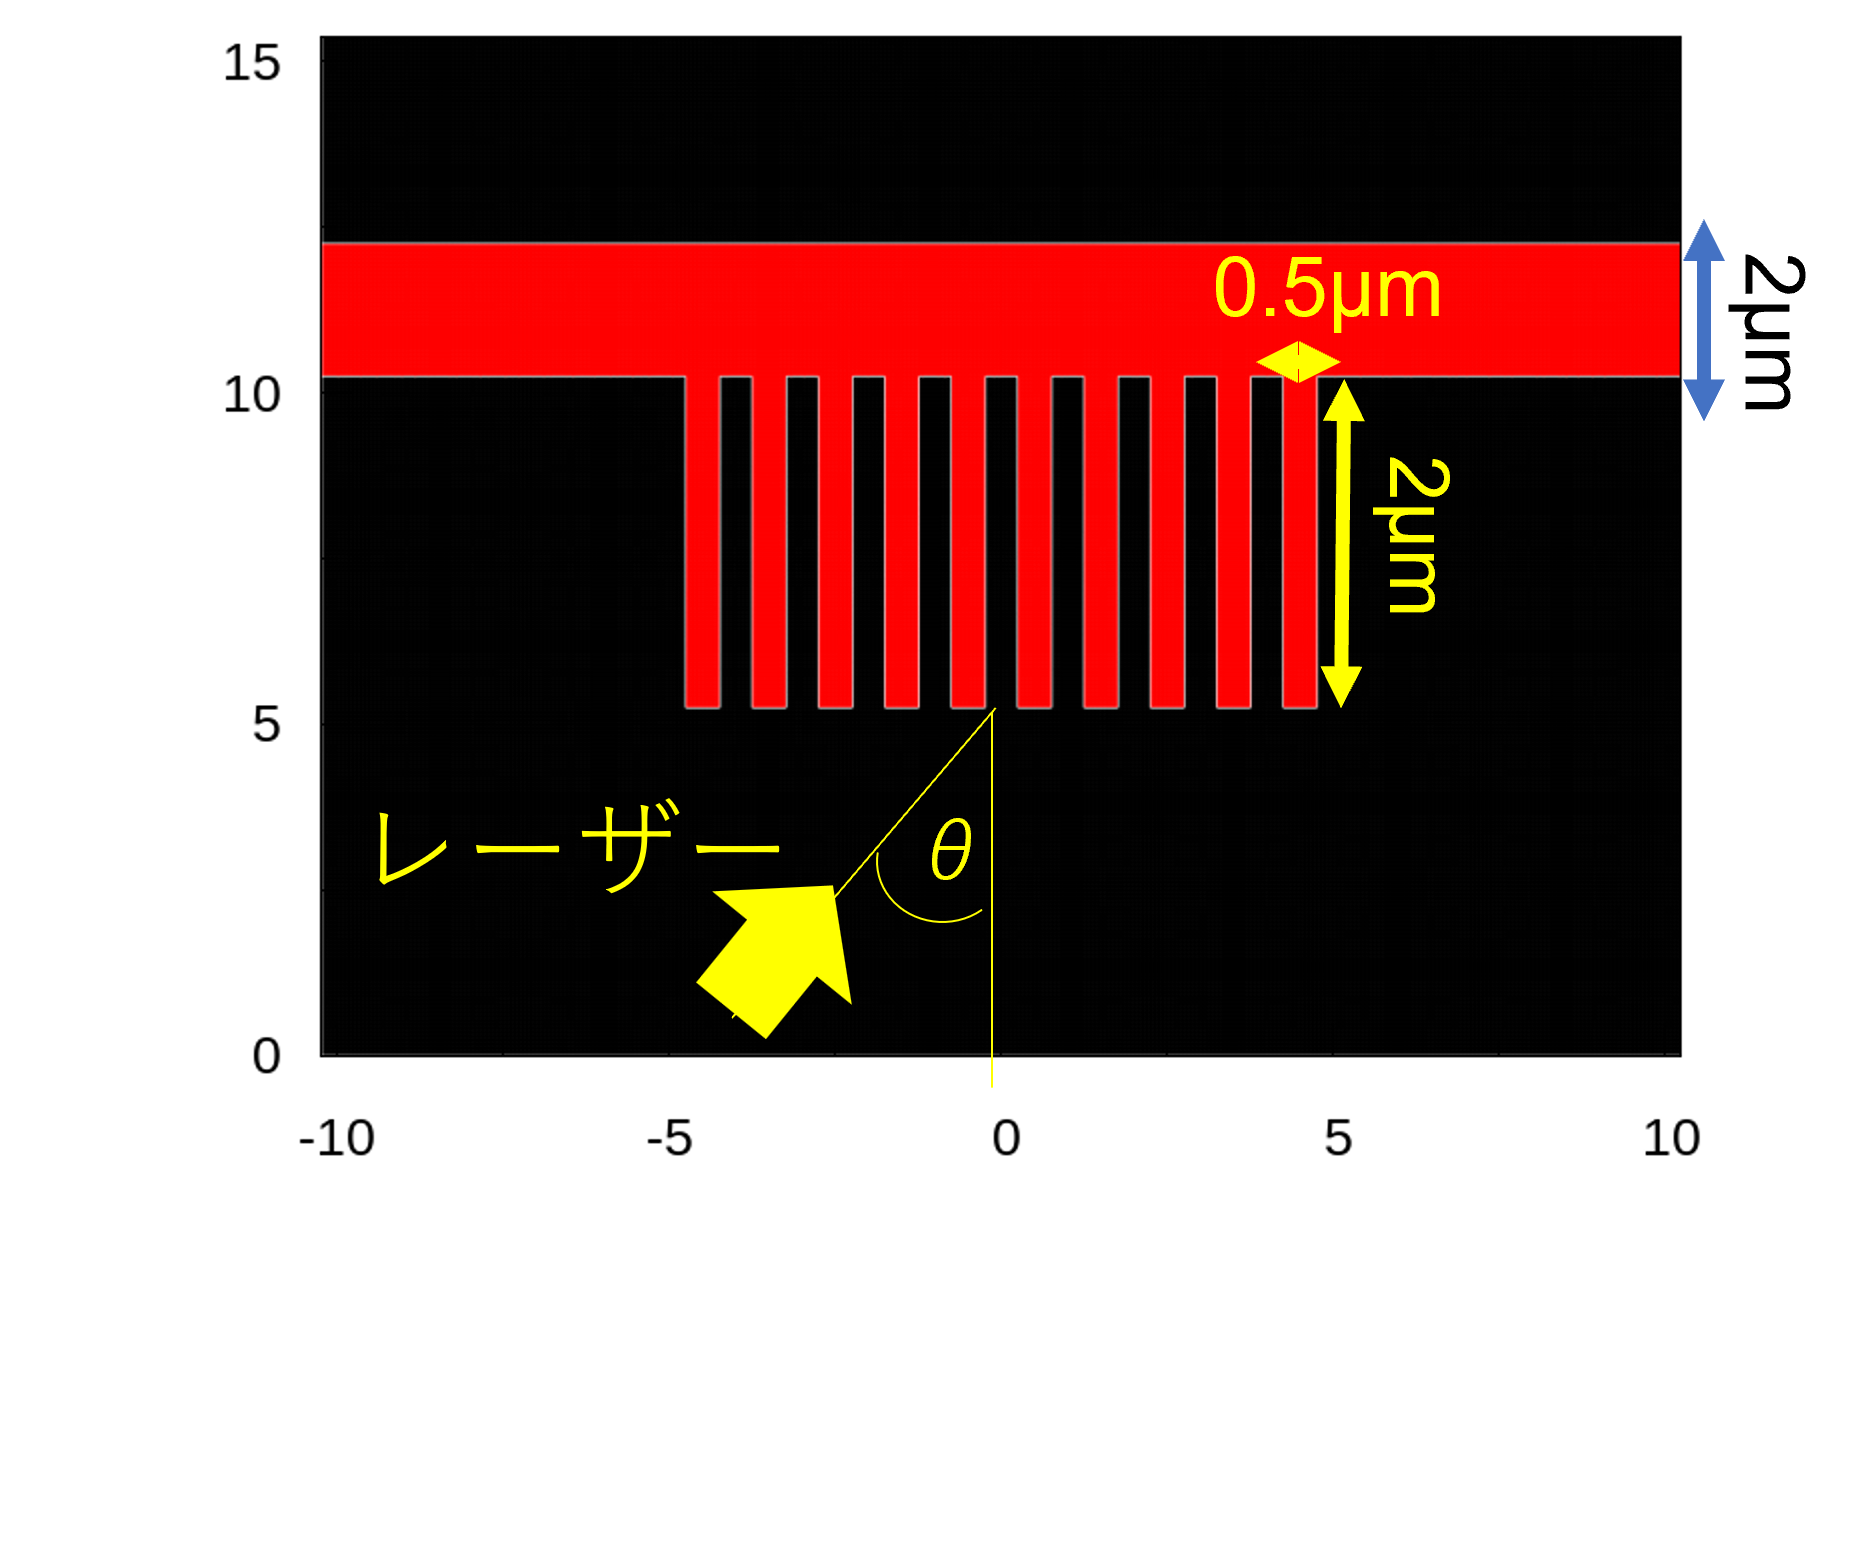
\includegraphics[scale=0.6]{./image/4-9-10rod.png}
    \label{fig:4-12}
    \caption{スラブターゲットと10本ロッドの図}
  \end{center}
\end{figure}

この系に対して、スラブターゲットに照射したレーザーと同様のパルス幅が 40 fs(FWHM)、最大集光強度がそれぞれ$1.2×10^{18}, 1.2×10^{19}, 1.2×10^{20}, 1.2×10^{21}W/cm^2$に達する高強度レーザーを +y方向から$\theta=$30度の角度で照射した。ここで、レーザーは y=40 nm に設置したアンテナから誘導電流を流すことにより発振させており、粒子 (電子とイオン)・場 (電場・磁場) ともに、xy 方向に透過(吸収)境界条件を課している。詳細なシミュレーション条件は表に示す。

\begin{table}[H]
  \begin{center}
    \caption{シミュレーション設定}
  \begin{tabular}{|l|r|} \hline
    \multicolumn{2}{|c|}{レーザー条件} \\ \hline
    レーザー強度 & $\textit{I}=1.2\times  10^{18},1.2\times  10^{19},$ \\ 
     & $1.2\times  10^{20},1.2\times  10^{21}[W/cm^2]$ \\ 
    規格化強度 & $\textit{a} _0 = 0.756, 2.39, 7.56, 23.9$ \\
    パルス幅 & 40fsec \\ 
    レーザープロファイル(波形)[時間方向] & ガウシアン \\
    レーザー空間分布 & 平面波 \\
    カットオフ密度 & $\textit{n} _c = 1.7 \time 10^21 [cm^{-3}]$ \\\hline
    \multicolumn{2}{|c|}{ターゲット条件} \\ \hline
    イオンの種類 & ケイ素(Si) \\
    電子密度 &$6.98 \times  10 ^{23} [\rm{cm}^{-3}]$ \\
    ロッド直径 & 0.5[$\mu$ m] \\
    ロッドの長さ & 10[$\mu$ m]  \\ \hline
    \multicolumn{2}{|c|}{系} \\ \hline
    システムサイズ(x方向) & [20.48$\mu $m] \\
    システムサイズ(y方向) & [15.36$\mu $m] \\
    メッシュ数(x方向) & [1024] \\
    メッシュ数(y方向) & [768] \\
    メッシュ幅(x方向) & [20nm] \\
    メッシュ幅(y方向) & [20nm] \\
    時間幅 & $1/6$[fs] \\ \hline
    \multicolumn{2}{|c|}{境界条件} \\ \hline
    粒子(x方向) & 周期 \\
    粒子(y方向) & 透過 \\
    電磁波(x方向) & 周期 \\
    電磁波(y方向) & 透過 \\ \hline
  \end{tabular}
  \end{center}
  \end{table}

  {準定常磁場生成}
  レーザー強度を変えた時の磁場の様子を示す。
  
  \begin{figure}[H]
    \begin{center}
      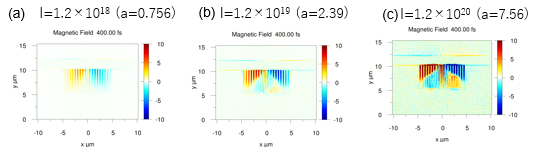
\includegraphics[scale=1.2]{./image/4-23-10rod.png}
      \label{fig:4-4-15}
      \caption{シュミレーション範囲内の磁場Bz。(a)はレ-ザーの強度が$I=1.2 \times 10^{18}$,(b)はレ-ザーの強度が$I=1.2 \times 10^{19}$,(c)はレ-ザーの強度が$I=1.2 \times 10^{20}$である。}
    \end{center}
  \end{figure}
  
  図\ref*{fig:4-4-15}からわかるようにレーザー強度を強くすると準定常磁場が強くなることがわかる。
  次にこの準定常磁場のエネルギーを比べる。
  
  
  \begin{figure}[H]
    \begin{center}
      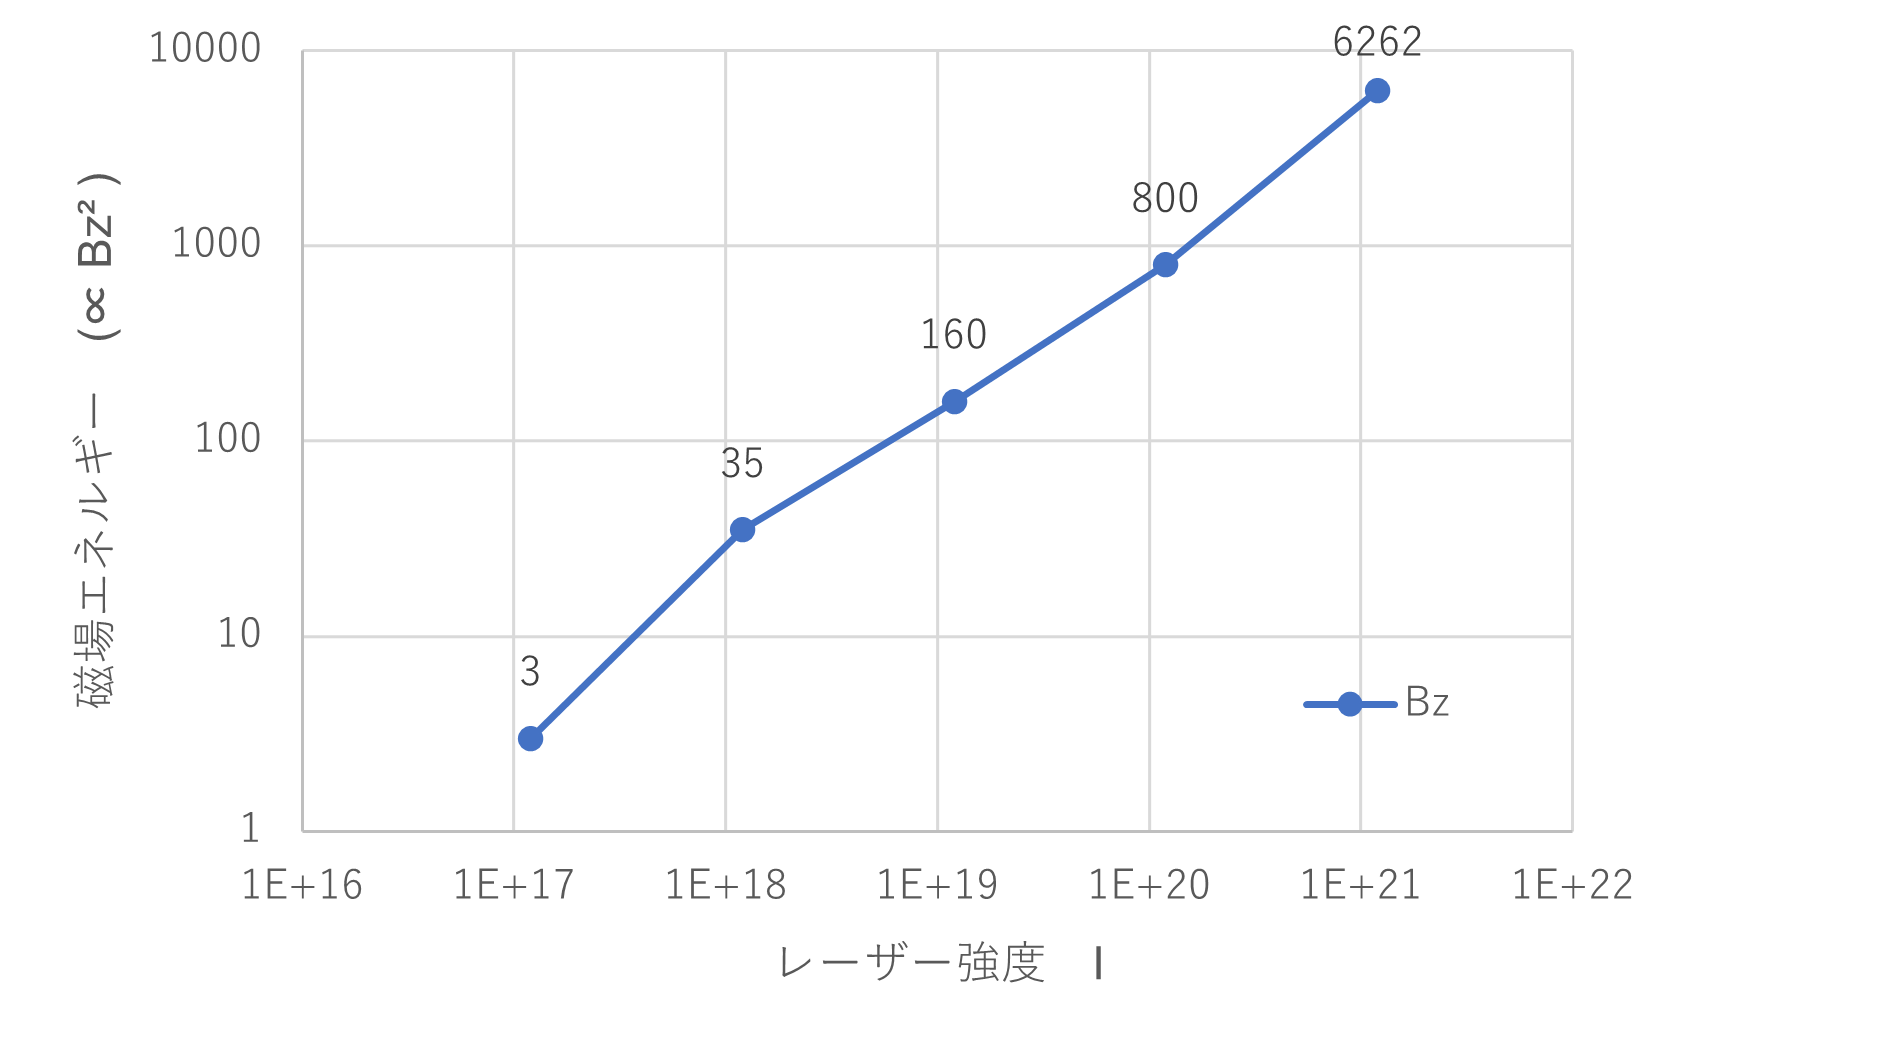
\includegraphics[scale=0.75]{./image/4-24-10rod.png}
      \label{fig:4-4-16}
      \caption{縦軸は磁場(Bz)エネルギー、横軸はレーザー強度を表している。}
    \end{center}
  \end{figure}
  
  図\ref*{fig:4-4-16}より、レーザー強度を強くすると準定常磁場が強くなることが数値的にもわかった。続いてこの準定常磁場が保存時間について示す。
  
  \begin{figure}[H]
    \begin{center}
      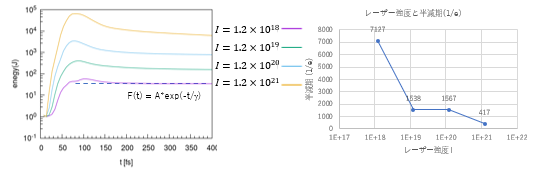
\includegraphics[scale=1.1]{./image/4-25-10rod.png}
      \label{fig:4-4-17}
      \caption{(a)は各レーザー強度ごとの磁場(Bz)エネルギーの時間発展の様子,(b)は(a)の時間発展の数値が$F(t)= A* exp(-t / \gamma)$の式のもと減少していくと仮定したときの半減期$\gamma$を表している。}
    \end{center}
  \end{figure}
  
  上図の(a)よりレーザー強度が大きければ磁場エネルギーは大きくなるが、一方(b)からわかるようにレーザー強度が大きくなれば半減期が小さくなり、磁場エネルギーの保存する時間が短くなることを表している。
  



%%%%%%%%%%%%%%%%%%%%%%%%%%%%%%%%%%%%%%%%% 5章 結論、今後の課題 %%%%%%%%%%%%%%%%%%%%%%%%%%%%%%%%%%%%%%%%%%%%%%%%%%%%%%%%%%%%%%%%%%%%%%%%%%%%%%%%%%%%%%%%%%%%%%%%%%%
\section{結論}

\subsection{まとめ}
物質に集光強度領域が$10^{18-21} \rm{W}/ \rm{cm}^2$のフェムト秒極短パルス高強度レーザーを照射することで、物質は即座に電離して電子が相対論領域となる高エネルギー密度プラズマが生成する。このとき、電子の相対論領域での運動により、プラズマ中にはメガアンペア(MA)に達する大電流が駆動され、キロテスラ(kT)の磁場が生成するとともに、イオンと電子との電荷分離に起因して数10 TV/mに達する電場が形成される。これらの強電磁場を伴うプラズマは、粒子線がん治療装置等の医療利用や核融合への応用が期待されるが、通常はレーザーパルスの時空間スケールで飛散し、電磁場もレーザーのパルス時間程度で消失する。我々は先行する粒子シミュレーション研究により、µmオーダの微細構造を付与した物質(構造性媒質)を用いることで、レーザーのパルス時間を越えた準定常な強磁場生成等、通常の固体薄膜等を用いた場合では見られない現象を見いだしている。これを踏まえ本研究では、相対論的電磁粒子コードEPIC3D\cite{m4}を用いて、構造性媒質として直径がサブµmオーダで高さが数10 mの円柱状ケイ素(ロッド)が複数配列した物質(ロッド集合体)を導入し、これに集光強度が1019 W/cm2の高強度レーザーをロッドの上面(軸方向)から30°傾けて照射する2Dシミュレーションを実施し、以下の結果を得た。\\
 (1)レーザー場がロッド集合体内部をTM波様に伝播することで、高エネルギー密度のバルクプラズマが生成する。伝播の過程で、(斜め照射に起因して)ロッド側壁が受けるポンデロモーティブ力に差異が生じることで、ロッド側壁に電流路が形成されることを明らかにした。その結果、、ロッドの間隙部分にkTオーダの強磁場が生成される。この電流は反磁性電流と同方向であり、レーザー通過後は反磁性電流と生成磁場による圧力平衡が成立する。この磁場はピコ秒の時間スケールで準安定に存在し、100 keVオーダのプラズマをパルス時間を数桁上回る長時間にわたり保持する機能を有することを明らかにした。\\
 (2)同一のレーザー照射条件において、空間充填率を保ちロッド径を0.125, 0.25, 0.5, 1.0 µmと変化させた場合にロッド集合体内部に生成する磁気エネルギーの時間変化を調べた。その結果、磁気エネルギーが最大になるロッド径が存在することを見いだした。さらに、レーザーの照射角度により生成磁場の向きおよび強度を調整可能であることを明らかにした。これらの結果は、ターゲットを工夫することでレーザーとの相互作用過程とレーザー生成高エネルギー密度プラズマ状態を制御できる可能性があることを示している。


\subsection{今後の課題}
高強度レーザーをµmオーダーの微細構造を付与したターゲットに照射すると、ピコ秒オーダーのスケールで準定常磁場が生成されることを示した。本研究では触れなかったが、ピコ秒オーダーになると粒子同士のコリジョンの要素が大きくなってくるため、コリジョンの効果を含めて計算をすることで、レーザーと媒質の相互作用をより詳細に理解することができると考えられる。また、本研究ではロッドターゲットのみ扱ったが、より長く磁場の保持させるという観点で適しているタ

%%%%%%%%%%%%%%%%%%%%%%%%%%%%%%%%%%%%%%%%% 参考文献 %%%%%%%%%%%%%%%%%%%%%%%%%%%%%%%%%%%%%%%%%%%%%%%%%%%%%%%%%%%%%%%%%%%%%%%%%%%%%%%%%%%%%%%%%%%%%%%%%%%
\newpage
  \begin{thebibliography}{999}
  \bibitem{ft1} T. H. Maiman, Nature $\bf{187}$,493 (1960)
  \bibitem{ft2} L. E. Hargrove, R. L. Fork, and M. A. Pollack, "Locking of hene laser modes induced by synchronous intracavity modulation, " Appl.Phys.Lett.$\bf{5}$,4 (1964).
  \bibitem{ft3} D. Strickland and G. Mourou, Opt. Commun. 56, 219 (1985).
% 19 20
  \bibitem{t19}A. S. Pirozhkov et al., Optics Express {\bf 25}, 20486 (2017).
  \bibitem{t20}H. Kiriyama et al., Optics Letters {\bf 43}, 2595 (2018).

  \bibitem{ft6} A. Macchi et al., Rev. Mod. Phys. $\bf{85}$, 751 (2013).

  \bibitem{100Mev1} F. Wagner $et\ al.,$ Phys. Rev. Lett. {\bf 116}, 205002 (2016).
  \bibitem{100Mev2} I. J. Kim $et\ al.,$ Phys. Plasmas {\bf 23}, 070701 (2016).
  \bibitem{100Mev3} A. Higginson $et\ al.,$ Nat. Commun. {\bf 9}, 724 (2018).

  %イオン加速
  \bibitem{ion_Acceleration}
  S. Inoue, $et\ al.,$, Phys. Rev. Lett. {\bf 109}, 1 (2012).
  \bibitem{ion_Acceleration_b}
  T. Esirkepov, $et\ al.,$, Phys. Rev. Lett. {\bf92}, 175003 (2004).

% TNSA
  \bibitem{10}
  E. L. Clark $et\ al.,$ Phys. Rev. Lett. {\bf 84}, 670 (2000).
  \bibitem{11}
  R. A. Snavely $et\ al.,$ Phys. Rev. Lett. {\bf 85}, 2945 (2000).
  \bibitem{12}
  S. C. Wilks $et\ al.,$ Phys. Plasmas {\bf 8}, 542 (2001).
  \bibitem{13}
  J. Fushs $et\ al.,$ Nature Phys. {\bf 2}, 48 (2006).
  \bibitem{14}
  B. M. Hegelich $et\ al.,$ Nature (London) {\bf 439}, 441 (2006).
  \bibitem{15}
  H. Schwoerer $et\ al.,$ Nature (London) {\bf 439}, 445 (2006).
% PRA
  \bibitem{16} T. Esirkepov et al., Phys. Rev. Lett.$\bf{92}$,175003 (2004).
  \bibitem{17} A. Macchi $et\ al.,$ Phys. Rev. Lett. {\bf 103}, 085003 (2009).
  \bibitem{18} C. Scullion $et\ al.,$ Phys. Rev. Lett. {\bf 119}, 054801 (2017).
  %CSA
  \bibitem{19}
  L. O. Silva $et\ al.,$ Phys. Rev. Lett. {\bf 92}, 015002 (2004).
  \bibitem{20}
  D. Haberberger $et\ al.,$ Nature Phys. {\bf 8}, 95 (2012).
  \bibitem{21}
  F. Fiuza $et\ al.,$ Phys. Rev. Lett. {\bf 109}, 215001 (2012).
  \bibitem{22}
  F. Fiuza $et\ al.,$ Phys. Plasmas {\bf 20}, 056304 (2013).
  \bibitem{23}
  H. Zhang $et\ al.,$ Phys. Plasmas {\bf 22}, 013113 (2015).
  \bibitem{24}
  W. L. Wang $et\ al.,$ Phys. Plasmas {\bf 23}, 073118 (2016).
  \bibitem{25}
  S. N. Chen $et\ al.,$ Sci. Rep. {\bf 7} 13505 (2017). 
  \bibitem{26}
  H. Zhang $et\ al.,$ Phys. Rev. Lett. {\bf 119}, 164801 (2017).


  % 慣性核融合
  \bibitem{NIF}O. A. Hurricane,$et\ al.,$ Rev. Mod. Phys. {\bf 95}, 025005 (2023).
  % 実験室宇宙物理
  \bibitem{28} F. Fiuza et al., Nat. Phys. 16, 916 (2020)
% PRE
  \bibitem{29} R. Matsui, Y. Fukuda and Y. Kishimoto, Phys. Rev. Lett. $\bf{122}$, 014804 (2019).
% CSBA
  \bibitem{30} R. Matsui et al.、水素クラスターを用いた求心衝撃波駆動 
  準単色プロトン加速(CSBA)レーザー学会学術講演会第40回年次大会
% 
  \bibitem{uehara} 上原直希, 京都大学大学院エネルギー科学研究科 修士論文(2019)
  \bibitem{ueda} 上田永樹, 京都大学大学院エネルギー科学研究科 修士論文(2022)
  \bibitem{higaki} 桧垣慎太郎, 京都大学大学院エネルギー科学研究科 修士論文(2022)(2023)
% IFSA
  \bibitem{IFSA} Y. Kishimoto et al., IFSA (2019), R. Matsui, Y. Fukuda and Y. Kishimoto, Phys. Rev. E 100, 013203 (2019).
% 18
  \bibitem{m4} Y. Kishimoto et al., J. Plasma Phys. $\bf{72}$, 971(2006).
% 17
  \bibitem{m3} S. Jinno et al., Plasma Phys. Control. Fusion $\bf{60}$, 044021 (2018).
% 13
  \bibitem{Kishi} Y. Kishimoto et al., Phys. Plasmas $\bf{9}$,589 (2002).

  \end{thebibliography}

\newpage
\section*{謝辞}
本研究を行うにあたり、丁寧かつ熱心なご指導を頂いた指導教官の石澤明宏教授及び、
岸本泰明名誉教授、今寺賢志准教授、この研究を進める上で終始助言や指導を頂いた松井隆太郎助教
、同研究室の皆様、本研究に携わって頂いた皆様に深く感謝いたします。\\ \\
\rightline{京都大学大学院 エネルギー科学研究科}\\
\rightline{エネルギー基礎科学専攻 修士課程}\\
\rightline{石原 聖也}

\end{document}
